\documentclass[a4paper,12pt]{scrartcl}

\usepackage[applemac]{inputenc}
\usepackage{verbatim}
\usepackage{paralist}
\usepackage{mathtools}
\usepackage{amsmath}
\usepackage[T1]{fontenc}
\usepackage[ngerman, english]{babel}
\usepackage{bibgerm}       		% german references
\usepackage{graphicx}
\usepackage{float}
\usepackage{cite}


%Das Paket erzeugt ein anklickbares Verzeichnis in der PDF-Datei.
\usepackage[hyphens]{url}
\usepackage{hyperref}

%Das Paket wird fŸr die anderthalb-zeiligen Zeilenabstand benštigt
\usepackage[onehalfspacing]{setspace}

\usepackage{textgreek}
\usepackage{amssymb}

%\newcommand\given[1][]{\:#1\vert\:}

%Einrueckung eines neuen Absatzes
\setlength{\parindent}{0em}

%Definition der Raender
\usepackage[paper=a4paper,left=30mm,right=30mm,top=30mm,bottom=30mm]{geometry}

% JavaScript Code Highlighting
\usepackage{listings}
\usepackage{color}
\definecolor{lightgray}{rgb}{.9,.9,.9}
\definecolor{darkgray}{rgb}{.4,.4,.4}
\definecolor{purple}{rgb}{0.65, 0.12, 0.82}
\lstdefinelanguage{JavaScript}{
  keywords={do, if, in, for, let, new, try, var, case, else, enum, eval, null, this, true, void, with, await, break, catch, class, const, false, super, throw, while, yield, delete, export, import, public, return, static, switch, typeof, default, extends, finally, package, private, continue, debugger, function, arguments, interface, protected, implements, instanceof},
  morecomment=[l]{//},
  morecomment=[s]{/*}{*/},
  morestring=[b]',
  morestring=[b]",
  ndkeywords={class, export, boolean, throw, implements, import, this},
  keywordstyle=\color{blue}\bfseries,
  ndkeywordstyle=\color{darkgray}\bfseries,
  identifierstyle=\color{black},
  commentstyle=\color{purple}\ttfamily,
  stringstyle=\color{red}\ttfamily,
  sensitive=true
}

\lstset{
   language=JavaScript,
   backgroundcolor=\color{lightgray},
   extendedchars=true,
   basicstyle=\footnotesize\ttfamily,
   showstringspaces=false,
   showspaces=false,
   numbers=left,
   numberstyle=\footnotesize,
   numbersep=9pt,
   tabsize=2,
   breaklines=true,
   showtabs=false,
   captionpos=b
}

\title{
A Blockchain-based Payment System for Microservices
}

\author{Florian G\"o\ss{}ler (mail@floriangoessler.de) @ ISE TU Berlin% <-this % stops a space
}

\begin{document}

% ---------------------------------------------------------------
    \thispagestyle{empty}
\begin{center}

\vspace*{1.2cm}
{\LARGE \textbf{Technische Universit\"at Berlin}}

\vspace{0.5cm}

{\large Chair of Information Systems Engineering (ISE)\\[5mm]}

Fakult\"at VII\\
Stra\ss{}e des 17. Juni 135\\
10623 Berlin\\

\vspace*{1cm}


\includegraphics[width=4cm]{Images/tu_logo.jpg}

\vspace*{1.0cm}

{\large Master Thesis}\\

\vspace{1.0cm}
{\LARGE \textbf{A Blockchain-based}}\\
\vspace*{0.25cm}
{\LARGE \textbf{Payment System for Microservices}}\\
\vspace*{1.0cm}
{\LARGE Florian G\"o\ss{}ler}
\\
\vspace*{0.5cm}
Matriculation Number: 366284\\
27.03.2018\\ % 	date of submission
\vspace*{1.0cm}

Supervised by\\
Prof. Dr.-Ing. Stefan Tai\\
\vspace*{0.5cm}
Secondary Supervisor\\
Prof. Dr. rer. nat. Sabine Glesner
\vspace{3cm}

\end{center}
   	\thispagestyle{empty}
    \cleardoublepage

    \thispagestyle{empty}
\vspace*{3cm}

\vspace*{1cm}
\noindent
First of all, I would like to thank Prof. Dr. Stefan Tai at the Chair of Information Systems Engineering for giving me the opportunity to carry out state of the art research in this field, and Markus Klems for his extrodinary support and feedback in his role as my supervisor.
\\
\\
Special thanks to my colleagues and managers at ImmobilienScout24. They made it possible to gain industry feedback and to work on my thesis in parallel to my daily tasks and responsibilities at ImmobilienScout24. Namely I would like to mention Tino Nitze, Enrico Kufhal, Richard Durnall, Franziska Schmidt and Robert Albrecht.
\\
\\
Furthermore, I want to thank my friends and family for supporting me in this long and hard times of working on this thesis. Your emotional support, as well as technical feedback and constructive discussions were of incredible value. Special thanks to Dr. Ann-Christin Gentschev, Peter Schrott and Tom Drenkard for their detailed feedback.

    \thispagestyle{empty}
    \cleardoublepage

    \newpage

\thispagestyle{empty}

\begin{large}

\vspace*{6cm}

\noindent
Hiermit erkl\"are ich, dass ich die vorliegende Arbeit selbstst\"andig und eigenh\"andig sowie ohne unerlaubte fremde Hilfe und ausschlie\ss{}lich unter Verwendung der aufgef\"uhrten Quellen und Hilfsmittel angefertigt habe.
\vspace{2cm}

\noindent
Berlin, 27.03.2018

\vspace{3cm}

\hspace*{7cm}%
\dotfill\\
\hspace*{8.5cm}%
\textit{(Signature Florian G\"o\ss{}ler)}

\end{large}
    \thispagestyle{empty}
    \cleardoublepage

    \thispagestyle{empty}
\vspace*{1.0cm}

\begin{center}
    \textbf{Abstract}
\end{center}

\vspace*{0.5cm}

\noindent

This thesis proposes a technical concept for a payment solution with which microservices can automatically charge each other for their provided services. The idea is motivated by the needs of cost transparency in large enterprises, as well as the applicability on decentralized web service marketplaces.\\

The proposed system is based on blockchain technologies and focuses on solving the performance and scalability issues that arise in conventional blockchain based systems. Therefore, a specialized state-channel approach was developed and a prototype was implemented to proof the concept and gain benchmark result. The prototype includes server and microservice client components, as well as a basic blockchain state and history inspection interface.\\

A strong focus is set on maintaining the trustlessness, security and decentralization properties, which are the largest benefits of a blockchain based solution, although these properties might not be required for all use-cases.\\

This work highly relates to general research about blockchain performance improvements, to cloud resource management and tracing, as well as to blockchain based machine-to-machine payment systems in other domains.

    \thispagestyle{empty}
    \cleardoublepage

    \thispagestyle{empty}
\vspace*{0.2cm}

\begin{center}
    \textbf{Zusammenfassung}
\end{center}

\vspace*{0.2cm}

\noindent

Diese Arbeit stellt ein technisches Konzept f\"ur ein Zahlungssystem vor, mit dem sich Microservices automatisch f\"ur ihre zur Verf\"ugung bzw. in Anspruch genommen Dienste bezahlen k\"onnen. Dies ist motiviert durch den Bedarf einer besseren Kostentranparenz in gro\ss{}en Firmen, sowie der M\"oglichkeit dies f\"ur dezentralisierte Webservice Marktpl\"atze zu verwenden.\\

Das hier vorgestellte System basiert auf Blockchain-Technologien und fokussiert sich auf die L\"osung der Performance- und Skalierungsprobleme, die normalerweise in blockchain-basierten System auftreten. Hierf\"ur wurde ein spezialisierter State-Channel Ansatz entwickelt und eine prototypische Implementierung umgesetzt. Einerseits um ein Proof-of-Concept zu liefern, andererseits um in Tests Leistungsbenchmarkergebnisse zu sammeln. Der Prototyp beinhaltet nicht nur Server und Microservice Client Komponenten, sondern auch ein Webinterface, um den Zustand und die Historie der Daten auf der Blockchain in diesem Kontext zu analysieren.\\

Es wurde Wert drauf gelegt, die Trustlessness-, Sicherheits- und Dezentralisierungseigenschaften, die zu den gr\"o\ss{}ten Vorteilen einer Blockchain basierten L\"osung z\"ahlen, nicht zu kompromitieren. Auch wenn diese nicht f\"ur jeden Anwendungsfall relevant sind.\\

Diese Arbeit steht in engem Bezug zur allgemeinen Forschung zum Thema Blockchain Skalierung und Performanceverbesserung, zu Cloud Resourcen Management, sowie zu Blockchain basierten Maschiene-zu-Maschiene-Zahlungsystemen in anderen Anwendungsgebieten.

    \thispagestyle{empty}
    \cleardoublepage

    \tableofcontents
    \thispagestyle{empty}

    \cleardoublepage
    \listoffigures
    \thispagestyle{empty}

% --------------------------------------------------------------

\newpage

\section{Introduction}

\subsection{Motivation}

More and more enterprises are using the microservice architecture \cite{web1}. This pattern is used to decouple services and increase flexibility. Individual teams are getting more independent in terms of technology stack and deployment. On the other hand, the number of interconnections between microservices increases.\\
These connections often connect microservices from different teams and departments with each other. For example, an infrastructure team might run a microservice that provides central user data. This service is then used by other teams for a checkout flow or a newsletter registration form.\\

Beside technical dependencies, this also introduces financial dependencies.\\

A providing service - like the user data service - creates costs for the team running it. First of all it must be developed and maintained, but it also incurs costs for hardware resources. In a cloud computing setting, this hardware is very transparent for the team itself. Also scaling a service, which requires more hardware resources, can be done easily when the load on the service increases. \\
However, consuming services and teams, like the checkout flow or the newsletter form, usually do not pay for the microservices they use as they consider them as a given resource ready to use.\\
Most often it is then the responsibility of managers of the providing services to negotiate for their budget. They need to justify, why their service is important and why they need a certain amount of money to run it. Often they need to do this without much data to prove their point.\\
Managers of consuming service, on the other hand, can falsely argue that their services are more efficient than they actually are. For instance, their service might just outsources all the heavy lifting to other microservices which can be used for free. The costs for this then do not appear on the balance sheets of the consuming services.\\
This scenario assumes a very hostile and competitive environment, which is not always the reality. However, this work explores a possible solution to this problem of intransparent financial dependencies. It can also be helpful in a friendlier environment, as well as in an inter-enterprise or web service marketplace setting.\\

These financial dependencies between services are important and could be a lot more transparent, for monitoring purposes and for budgeting processes, as mentioned above.\\

To visualize these dependencies, a lot of data needs to be collected and evaluated. A straightforward approach would be to count all requests that are made to and from a service. This counting can happen in a fine granularity to be able to investigate connections on a per service level and in specific time intervals.\\
Since this data shall be used for financial evaluations and operations, it is highly sensitive, so it should be impossible to manipulate or delete it. The data must be gathered in a way that does not rely on a trust relationship between any two participants.\\
Having all this data transparently available, teams can start to optimize their services for efficiency and profit. Eventually every development team can measure themselves against a concrete monetary goal. Every team can "make profit" \cite{web3}. This market oriented approach increases the urge for efficiency from which the whole company can benefit \cite{png2013managerial}.\\

For example, consider a user data service and a checkout flow: In multiple of the steps of the checkout flow user data is required. A naive implementation would load the user data from the user data service for every step. This causes load on the user data service which needs to perform database lookups and other operations to provide this data. It might have been the more straightforward implementation for the developers of the checkout flow. However, costs could be reduced, when the checkout flow caches the user data once they were retrieved and does not create load on the other service anymore. This reduces the required computing power of the user data service. If the user data service charges for every request, this cost is transparent, and the consumers of this API (Application Programming Interface) are more motivated to use it wisely.\\

A system, which is able to securely create microservice usage reports, would not be limited to any one enterprise: when this system is run internally, it could be expanded for the dependencies to external partners. In turn, the external partners could bill the enterprise based on these reports for the actual usage.\\

Thinking in an even larger context, one could imagine a public marketplace of services where services bill each other through this system.

\subsection{Goal}

This master thesis aims to explore a possible technical design and prototypical implementation for the outlined pay-per-use scenario. For this, a secure and stable payment infrastructure is needed.\\

Blockchain technologies promise to enable a distributed ledger and payment system, which can be used for a variety of use cases \cite{web5}. They especially provide payment systems where the individual parties do not need to trust each other or a third party to perform secure transactions. This makes it an interesting choice as the foundation of the payment infrastructure.\\

\textbf{The goal is to develop and evaluate a blockchain-based payment system, that is suitable for modeling and monitoring financial dependencies in microservice architectures.}\\

The special challenge with this is the high-volume of payments that need to be performed and the large amount of data that needs to be evaluated in this machine-to-machine interaction scenario, backed by a blockchain as single point of truth.

\subsection{Requirements}

To be considered suitable the system needs to fulfill a series of requirements.\\

Functionally it needs to be able to:

\begin{itemize}
\item[] \textbf{F1) Perform payments between services on a per request basis.}
\item[] \textbf{F2) Keep a log of the number of requests within a certain timespan.}
\end{itemize}

F1) The payment needs to be ensured before the service provider responds with an answer. The payment does not need to be executed by then, but the provider needs to be sure that he will be paid eventually.\\

F2) This log enables the system to provide information about the interaction patterns between the services.\\

The non-functional requirements for the system are:

\begin{itemize}
\item[] \textbf{N1) Security}
\item[] \textbf{N2) Trustlessness}
\item[] \textbf{N3) High Performance}
\end{itemize}

N1) Security in this context is defined as the property to be resistant against manipulation and fraud. The service provider needs to be sure that the service is getting paid for. Also the service consumer should have a guarantee for payed expenses. Neither a third party should be able to manipulate transactions nor one of the transaction participants.\\

N2) A trustlessness system is defined as a system in which the provider and consumer do not need to trust each other or another third-party intermediary for the payment process, but only in the protocol and implementation of the system.\\

N3) The system needs to deliver high performance since microservice systems can be used in environments where hundreds of interactions per minute are the norm. The system must run along the normal service operation. It cannot rely on a sampling or a post-processing approach to perform the payments to ensure that every request is paid.\\
Two performance metrics are most relevant in this scenario: The request latency and the throughput of requests.\\
Latency: The payment process shall not increase the request response time of a service by a too large amount.\\
Throughput: The whole payment system needs to be able to process a large number of requests per minute.\\
Exact numbers and thresholds highly depend on the usage scenarios and amount of services that communicate with each other.\\

In the context of this thesis three usage scenarios are considered:

\begin{itemize}
\item \textbf{Enterprise}: The system is used only within a single organization.
\item \textbf{Hybrid / Permissioned}: It is used within an organization and its partners.
\item \textbf{Public}: Anyone can join the system.
\end{itemize}

The requirements stay the same across the three projected usage scenarios, but are relevant to different degrees.\\
The level of trust decreases dramatically with the number of participants as visualized in figure \ref{fig:TrustLevelGraph}. With a decreasing level of trust, the importance of the security (N1) and trustlessness (N2) properties become more important.\\
For an enterprise setting only, this system might sound too heavy. However, in this thesis the goal is to evaluate a system, that fits all three settings and therefore must be able to handle a very hostile environment.

\begin{figure}[H]
\centering
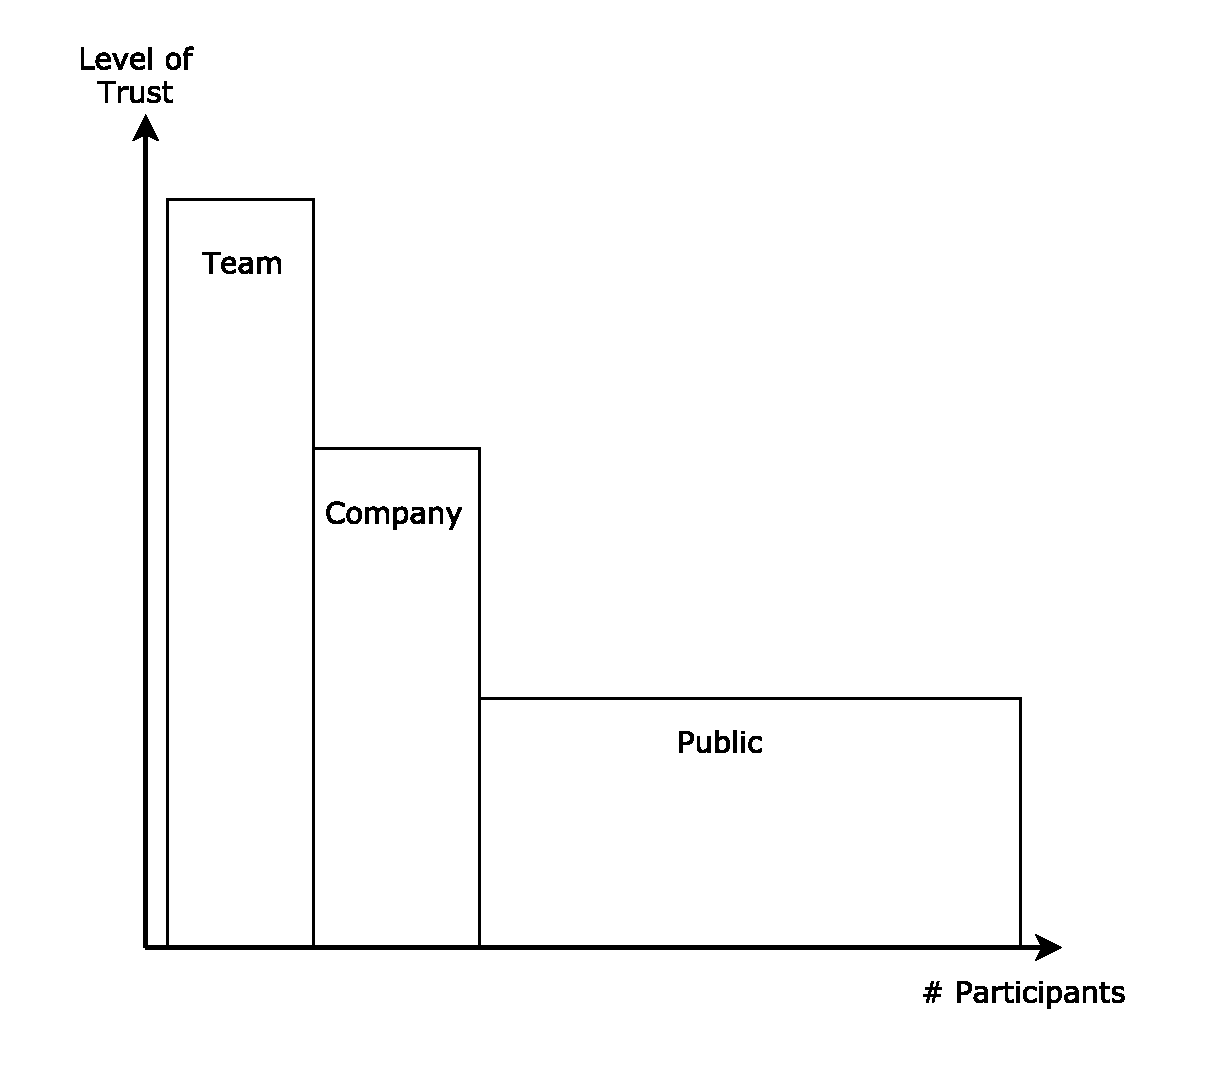
\includegraphics[width=300pt]{Images/TrustLevelGraph.pdf}
\caption{Trust Level.}
Intuitively the more participants are part of a group the lower the general level of trust among any two random participants. This graph shows three example groups: a software development team (high level of trust), a company (medium level of trust) and the public (low level of trust).
\label{fig:TrustLevelGraph}
\end{figure}

\subsection{Stakeholder Feedback}

To evaluate the potential relevance of such a system in a real world microservice, system several stakeholders at ImmobilienScout24 were interviewed. ImmobilienScout24 is Germany's leading marketplace for real estates and related services with over 12 million visitors per month \cite{web97}. It is running a hybrid infrastructure with own data-centers and cloud services provided by Amazon Web Services (AWS) \cite{web38}, while its sister portal AutoScout 24 is migrating to a full cloud infrastructure right now. Beside some technical team leads, developers and tech operation personal, also the Chief Technology Officer (CTO) was interviewed.\\

The interviews were quite informal and took about 30 minutes. Each interviewee received a short presentation about what challenges the system should help with and how it works. The amount of interviewees is too small, to have a statistically relevance and this is no attempt of a quantitative analysis. The goal was to get some insights from an industry perspective.\\

Overall, all participants were very interested in the system and positive about it. State of the art budgeting processes often seem to be an educated guess with a lack of insights in the actual operational costs, needs and dependencies. Several attempts were made to analyze costs of services but dependencies between services were not part of such attempts yet. All stakeholders agreed that more transparency is desirable.\\

The cost transparency level also differs between services that run in the data center and ones that run in the cloud.\\
For services in the data center, individual costs are hard to measure accurately because of the complexity of different hardware requirements and usage patterns of shared resources. The operations team tried to calculate average prices per server instance per month to give some kind of transparency to the individual teams. These numbers are also used to evaluate whether a service should be moved to the cloud and to compare cloud vs. data center costs.\\
For services that run in the cloud costs are more transparent already. Each team or function group receives its own AWS account. With this separation and an additional tagging system, individual resources can be assigned to specific teams. Through this, teams can monitor their costs and start to optimize them.\\
However, in neither setting are dependencies between service tracked in terms of costs.\\

Current projects start to raise questions about cost of dependencies. For example, a sophisticated machine learning project was a joined project of the real estate financing team and the data science teams. It involves several components running in different AWS accounts. For now parts of it are tagged as "belongs to finance", while other parts are tagged as "belongs to data science". Through this, some kind of artifical cost split is achieved. However, more features from additional teams shall be integrated in this system in the near future. The cost split is an open question here.\\

The security aspect of the payment system was valued by the stakeholders. Especially when using the system not only for monitoring but with real or even automated budgets. However, their most valued feature is the increased transparency and reliability. Current logging system are not used consistently and are also not reliable enough to extract similar information. The payment system would enforce the existence of this dependency data.\\

The stakeholders raised special concerns about the performance of the system. A significant, by the user noticeable impact, on normal operation should be avoided. Also, the system must be easy to integrate because it would otherwise never reach a widespread adoption. Other concerns were raised for the case of services that are used internally by other microservices but also publicly from a user's browser or third parties. Securing those services with a payment system raises additional challenges.


\subsection{Background}

The following outlines some concepts and technologies that are used as the foundation for this thesis.

\subsubsection{Microservices}

The term "Microservices" describes a software architectural pattern, that structures an application as a set of loosely coupled services \cite{web2}. The services should be small, focused and lightweight. Protocols for interaction need to be implementation independent to enable reuse, refactoring and exchange of services. This architecture enables great reuse of existing functionalities. The increased modularity also makes the application easier to develop, test and maintain for individual, independent, focused teams. Also continuous delivery and deployment are easier to achieve.\\
This architecture is related to Service Oriented Architectures (SOA) \cite{kart2009managing} but should be clearly differentiated from it \cite{Birk2016}. SOA tends to create larger services and often involves more formalities.

\subsubsection{Cloud Computing}

Cloud computing enables the access to a shared pool of customizable computing resources, like servers and storage, but also to ready-to-use service abstractions like databases, event queues and more \cite{web40}. This is done in a ubiquitous and convenient way, on demand via network access and allows for rapid provisioning and release. Another important property is that it involves minimal management effort and service provider interaction.\\
This enables a high level of flexibility for companies to scale their services based on actual demand and rapidly develop new services and products. It also avoids up-front infrastructure cost and enables businesses to focus on their core competences.

\subsubsection{Blockchain}

A "blockchain is an open, distributed ledger that can record transactions between two parties efficiently and in a verifiable and permanent way." \cite{iansiti2017truth} All transactions are captured in so called blocks. These blocks are created - also called "mined" - by the network and are cryptographically sealed. A block usually contains a set of transactions for a certain time span. Subject to the used blockchain protocol and configuration, this time span is usually within the range of seconds or minutes. Each block is based on its predecessor. This creates a chain of blocks - hence the name. Each block contains the hash value of the previous block. Because of this dependency and the cryptographic sealing, manipulation of an existing block down the chain would require a change of all successor blocks. This breaks the chain, which would reveal the manipulation attempt.\\

To mine these blocks and ensure that all nodes agree on the same set of transactions in a block, a consensus algorithm is required. Most systems rely on a proof-of-work \cite{web47} algorithm, which forces the nodes to solve a cryptographic puzzle. Other approaches like proof-of-stake \cite{web47} or proof-of-authority \cite{web48}, which is only reasonable in private networks with trusted authorities, are also possible.\\

A blockchain can also be seen as a large distributed database without a central administration, where transactions are the records of state changes. In a trivial case this state change transfers a value, like Bitcoins, from one party to another. In more sophisticated chains these transactions can carry additional metadata or even execute small programs.\\

Blockchains can be characterized as SALT systems \cite{Tai2017}. From a transaction perspective, SALT stands for sequential, agreed, ledgered, and tamper-resistant. From a systems perspective it can be described as symmetric, admin-free, ledgered, and time-consensual. Especially the properties sequential (one transaction after the other), ledgered (a transaction cannot be undone and is agreed upon by all nodes) and tamper-resistant are relevant for the proposed payment system.\\
This stands in comparison to traditional database system, which usually support ACID transactions (Atomicity, Consistency, Isolation \& Durability) \cite{gray1992transaction}, or NoSQL stores for high performance web applications, which are characterized as BASE (Basically Available, Soft state, Eventually consistent) \cite{brewer2000towards}.\\

The data of all blocks including all transactions is replicated to every full computing node in the network. In some systems also shallow nodes are possible. These only store a checkpoint reference and recent blocks. This replication makes the system highly resilient because data cannot get lost or manipulated. However, this also creates a lot of overhead. The blockchain size increases over time and already takes up several gigabytes for popular blockchains.\\

Blockchains provide even more benefits like empowered users, transparency and low cost, and fast transactions compared to other transaction systems \cite{web5}. On the other hand, they also face some challenges like high energy consumption, privacy concerns and an unclear regulatory status \cite{web5}.\\

Usually blockchains operate as a large public network, but it is also possible to run a private network with restricted access. This is useful for testing, as well as for networks inside of organizations to serve a dedicated purpose.

\subsubsection{Asymmetrical Cryptography}

Asymmetrical cryptography is an essential part of the modern communication infrastructure.\\
It is based upon the fact that each participant owns two keys. A private key and a public key. As the names imply, the private key shall only ever be known by the participant himself. The public key, however, can - and should - be available publicly.\\
For example, if Alice wants to send Bob a secret message, Alice would use Bob's public key to encrypt the data and then send it through a possible insecure channel. So only Bob (the owner of the private key) can decrypt the message.\\

A signature \cite{salomaa2013public} on the other hand uses a reversed process. It ensures that only whoever had access to the private key can be the author of a signature that is attached to a piece of data. For this the signature is generated with the private key of the sender over the message data. This signature is then sent along with the message. A receiver can then use the public key of the sender with the message and the signature to verify that it was actually sent by the sender and that no attacker modified it on the way.

\subsubsection{Smart Contract}

A smart contract in the context of blockchains is a small executable program that can be deployed on the chain \cite{web9}. It can then be triggered by transactions, store data and even receive and mange funds. Not all blockchains support such a feature and it is not trivial to implement.\\
A smart contract can define a set of rules for the interaction between parties that are automatically checked. It can be seen as a codified, executable version of a classic paper contract.\\

This enables a lot of use cases that go beyond the bare exchange of monetary values like Bitcoins. For example, a contract can be defined that only pays out a certain amount if another condition is met. It is also possible to implement a voting system with it, which only performs a transaction if a certain threshold of agreement was reached.\\

Eventually smart contracts could make existing, complex and often not mathematically precise paper contracts obsolete or at least extend them.
Further research exists about this \cite{Egbertsen2016}. Another interesting research topic about such contracts is on how to create a financial domain specific language to express financial agreements via smart contracts \cite{Biryukov2017}.

\subsubsection{Ethereum}

Ethereum \cite{web7} is a very popular blockchain nowadays. In terms of transaction volume and value of the currency it ranks second after Bitcoin \cite{web22}. Its currency is called Ether.\\

Ethereum supports smart contracts in a variety of dedicated programming languages. These are compiled to a bytecode representation, which is executed on the nodes of the network. Smart contracts in Ethereum are turing complete. This provides a complete programming model with loops, branches and statement and that therefore any algorithm can be implemented. To avoid a deadlock of the system by long running or even never terminating contracts, each computation step consumes a certain amount of a virtual resource called gas. Gas is paid for with ether based on market demand. The cost for it is therefore part of the overall transaction cost. If a transaction is submitted to the network an amount of gas must be sent along. If that amount of gas is not sufficient enough to execute the transaction, it will be declined and will not be mined into the blockchain.\\

The support for smart contracts is an essential difference to Bitcoin. Also other issues that were discovered in the Bitcoin protocol were addressed \cite{web8}.

\newpage
\section{Related Work}

This thesis relates to several topics in the space of distributed ledger research as well as the field of distributed systems. Some of these topics are areas where this system can be applied. Others have a similar approach, but in another domain or context. Some also provide technical or conceptual foundations on which this system is built upon. Figure \ref{fig:RelatedWork} gives a brief schematic of the classification before this chapter will go into more detail them - especially about Blockchain Throughput Scaling.

\begin{figure}[H]
\centering
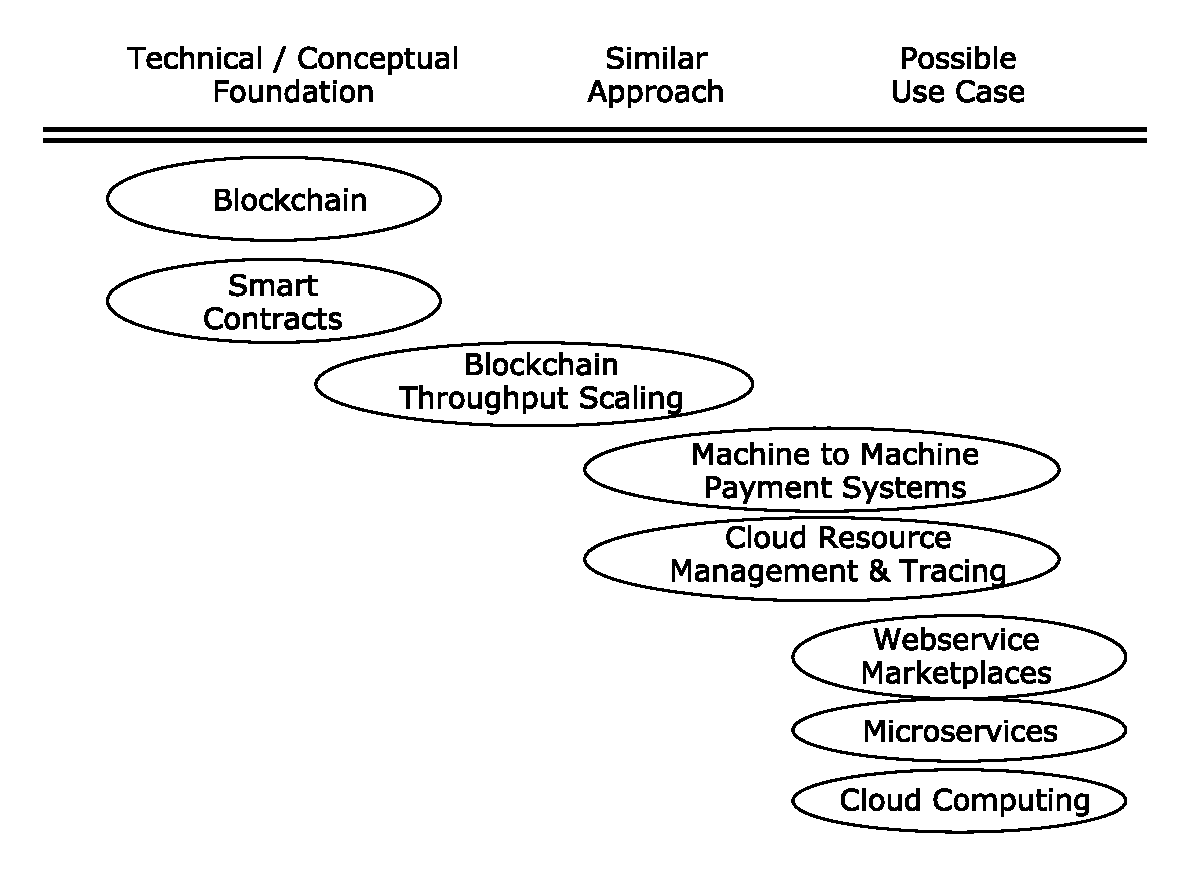
\includegraphics[width=450pt]{Images/RelatedWork.pdf}
\caption{Classification of background and related work topics.}
\label{fig:RelatedWork}
\end{figure}

\subsection{Web Service Marketplace}

A web service marketplace is a system that allows web services from different providers to be found, connected to and purchased. Ideally this can happen in a very automated fashion. Providing services for others to use is a potential business model and not a new one. Such a market place could be the ultimate use case for an automated trustless payment system.\\
When Service Oriented Architectures (SOA) \cite{kart2009managing} were first discussed the idea of marketplaces to exchange digital services was present \cite{Hartmanis2007a}\cite{Papazoglou2003}. The topic was also revived by the Software as a Service \cite{Kumar2017} trend \cite{Cusumano2010} \cite{turner2003turning}.\\
However, only marketplaces with limited impact could be established yet. Examples are Saleforce's force.com \cite{web58}\cite{Weissman2009} or SAP's YaaS \cite{web59}.\\
One could aim for a system with a similar impact as the app stores for iOS and Android devices, which had a big impact on how consumers purchase software today.\\
An effect that was often observed in attempts to create a marketplace, was the attempt to achieve a certain level of vendor or marketplace lock in. The marketplaces were specialized, and therefore the usage of the provided tools and frameworks was required to participate. This blocked an open usage, although open standards to achieve technical interoperability, like the Web Services Description Language (WSDL) \cite{web64}, were developed early. It is seen as a necessity that marketplaces stay open to really achieve their true potential and are not just another way to deliver a traditionally packaged software product \cite{Cusumano2010}.\\
It might be possible, that the central position of a marketplace, not only for the connection of the services but especially for the payment processing, hurts an open approach. A decentralized and automated payment system, like proposed in this thesis, could solve parts of this problem.\\
Also research exists about the effects of marketplaces for digital services \cite{Schlauderer2011} as well as for intermediaries in digital markets \cite{Giaglis2002}. Related research also investigates the effects of online anonymous marketplaces \cite{Soska2015} like "Silk Road" \cite{web68}.\\

A truly open marketplace would be a future use case for the system developed in this thesis because it requires the possibility for secure and trustless payments. A marketplace with time-based access payments via a blockchain was already investigated by researchers at the TU Berlin \cite{klems2017trustless}. However, it does not provide the possibility of per usage payments.\\

\subsection{Machine-to-Machine Payment Systems}

In other areas than server-to-server communication, machines also need to be able to pay other machines without user interaction.

An example for such an area is the space of Internet of Things (IoT). Distributed sensors from different parties shall communicate in big networks to provide data about the real world via their sensors. Here blockchain technologies are evaluated to financially reward these small IoT devices and protect against fraudulent participants \cite{worner2017impact}. Special challenges arise here from the power consumption constraints, low bandwidth networks and transaction times.

Also in the area of smart power grids and electrified roads, machine-to-machine payments between power providers and power suppliers or cars and infrastructure are desirable. Again, blockchain concepts are already evaluated \cite{Hagstrom2017}, where similar scaling issues and transaction time limits also apply.

\subsection{Blockchain Throughput Scaling}

Blockchains are a highly reliable and secure way to store information but they are not good for high throughput. Because of the computational expensive consensus algorithms, especially proof-of-work, the number of transactions is limited, and a transaction usually takes seconds or even minutes until it is mined and confirmed.\\
There are several approaches to scale blockchains for higher throughput and lower latencies. The following is not a full list, but a collection of approaches which can be repeatedly found and were considered for this thesis.

\subsubsection{Tuning Blockchain Parameters}

The most naive but also limited approach to the scaling problem is, to tune the blockchain parameters \cite{Croman2017}. For example, Bitcoin uses a ten minute block time - the interval in which new blocks are mined - and a block size of up to one megabyte. The throughput can be improved by reducing the block time - yielding more blocks per time - or increasing the block size - yielding more transactions per block. Block time reduction would also improve the latency. This is an example of the ongoing discussions in the Bitcoin community and cause of forks like Bitcoin Cash \cite{web83}.\\
This however, is just a minor patch and does not solve the scalability problem on the long run or for high frequency and low latency (below one second) requirements.

\subsubsection{Sidechains}

The idea of sidechains is to offload work from the main chain into a dedicated blockchain that is linked to the main chain \cite{Back2014}\cite{Croman2017}. These sidechains can be implemented with a greater freedom of choice in their consensus algorithm and lower decentralization. However, they face some challenges in terms of interoperability with other chains which may cause higher delays and additional transactions on the main chain for inter-chain transactions.\\
Sidechains also do not solve all scalability issues since they are essentially just a dedicated blockchain with a smaller number of nodes and transaction scope.

\subsubsection{Sharding}

Sharding \cite{Croman2017} is a technique popular in the database field. Instead of each node in a network being responsible for the whole data a node only stores and validates one or multiple parts of the data - so called shards. These shards are still replicated to multiple nodes, but not to all, increasing the performance, due to the reduction of the communication and storage overhead, since not every node needs to know everything.\\
Several approaches to sharding for blockchains exist \cite{Li2017}\cite{Gencer2017}\cite{kokoris2017omniledger}\cite{luu2016secure} but it also imposes special challenges to ensure that shards are distributed without impacts on the trust level and for transactions that span multiple shards. For example, the system must be protected against the case that a shard could be manipulated by a single party, who controls the majority of nodes that are responsible for this shard.

\subsubsection{Permissioned Blockchains}

Permissioned, or also called private, blockchains restrict the access to the chain itself. This stands in a strong contrast to the open nature of the big public blockchain networks like Bitcoin and Ethereum which anyone can join.\\

Restricted access can tackle multiple issues with public chains. First of all, the chain can contain and handle more sensitive data, since it can be designed to not be publicly readable. The chain can also focus on other use-cases than just payments and specialize for them. By having a dedicated chain for a certain use-case, nodes do not need to deal with irrelevant public transactions of other domains. Because of the constrained set of participating nodes, other consensus algorithms than expensive proof-of-work algorithms can be used. This can improve the throughput significantly \cite{Pongnumkul2017}.\\

For example, a Byzantine Fault Tolerance (BFT) consensus algorithm can be used. Byzantine fault tolerance \cite{Jackson2005} relates to the byzantine generals problems stated by Lamport \cite{Lamport1982}. This problem states the challenge of achieving a consensus among a set of communicating individuals from which some might act faulty and deliver - intentionally or unintentionally - wrong information to their peers.\\
BFT algorithms seem to be promising for blockchains in terms of scalability up to a certain number of nodes \cite{Vukoli2016}\cite{Sousa2017}.\\

The Hyperledger project \cite{web89} aims to develop a framework for business ready enterprise permissioned blockchains and is a project of the Linux Foundation. Especially IBM invests heavily in its Hyperledger Fabric \cite{Cachin2016}. With Ethereum, it is also easily possible to create a private network \cite{web91}.\\

Microsoft announced a blockchain enterprise framework called Coco \cite{Coco2017}, which can be connected to various blockchain implementations. It aims to be used in a consortium of enterprises where nodes can be somewhat trusted. Their system is based on the existence of a secure execution environment (e.g. Intel's SGX \cite{web20} or Windows Virtual Secure Mode (VSM) \cite{web21}), which handles the critical parts of the transactions. This approach is supposed to dramatically increase throughput. In the initial test, mentioned in the whitepaper, the throughput could be increased to about 1600 transactions per second. Beside performance improvements Coco also addresses confidentiality concerns.\\
Coco achieves all this with security tradeoffs and stepping away from the truly decentralized, trustless blockchain approach based on strong consensus algorithms. It is to be evaluated whether Coco still provides enough advantages over traditional enterprise systems. It drops some essential blockchain properties but still causes additional implementation and runtime overhead for the blockchain.\\
Coco was not further considered for this thesis since it was not yet available and drops essential properties that violate the requirements for the prototype.

\subsubsection{Off-chaining}

There are several patterns on how to put transactions or parts of the logic of smart contracts off the blockchain and thereby increase the throughput or reduce latencies. These patterns cover different use-cases and usually trade in properties of the blockchain to a certain degree. Eberhardt and Tai   \cite{eberhardt2017or} provide a comprehensive overview of the most common patterns, which are briefly summarized here.\\

First of all, they mention the \textbf{"Challenge Response Pattern"} \cite{eberhardt2017or}. There, the smart contract models a state machine with well-defined final states. Determining whether a state is final might be an expensive operation but performing a state transition is computationally cheap. A client can now claim that a state is final at any point. Any other client can prove them wrong if they can provide a valid state change. An example for this is a chess game. One player can claim the final state of setting the other player check mate. This would be too computational expensive to prove on chain in a smart contract. But the other player can provide a valid move to continue the game if the claim was wrong. Timeouts are needed in this approach to avoid a deadlock if one client becomes unavailable forever or for a too long period.\\
This pattern is great to move complex computations off-chain or generally handle situations where one party claims something against another.\\

\textbf{"Content-Addressable Storage Pattern"} is a pattern that Eberhardt and Tai \cite{eberhardt2017or} describe, which is used to solve the problem of storing large amounts of data on the blockchain. Instead of storing the data itself on the blockchain, just an address and a cryptographic hash are stored on the blockchain. The address indicates where the actual data can be found. The hash is generated over the data and can be used to verify the integrity of the data.\\

Under the term \textbf{"Low Contract Footprint Pattern"} Eberhardt and Tai \cite{eberhardt2017or} summarize the general effort to reduce the amount of computing steps and checks in a smart contract to an absolute minimum. The smart contract's internal data structures should be optimized for space and efficient write operations. Read operations are free of transaction cost. Anything that can be inferred from existing data should not be stored again. Also checks on preconditions for a transaction should be performed off-chain first and the transaction should only be executed on chain, if the precondition check passes and the transaction therefore has a very high probability of actually succeeding.\\
It should be mentioned that this is not a real off-chaining pattern and usually is already done intuitively. The system developed during this thesis takes these considerations into account.\\

Another approach to perform interactions between two actors off-chain, is described as \textbf{"Off-chain Signatures Pattern"} \cite{eberhardt2017or}, which is also known under the term \textbf{"state channels"} \cite{web13} or \textbf{"payment channel"}. Here a smart contract is deployed for the interaction between two actors. The contract includes a function that accepts a new desired state as argument and updates its current state that is stored on the chain with it. This submitted state change must be cryptographically signed by both actors. Otherwise the contract will deny the state change. In a simple example the state is just a representation of how much of the funds inside the contract belongs to whom. If at the beginning both own 20 tokens each and Alice wants to send Bob ten tokens, she can create a state change that specifies her stakes at ten and Bob's stakes at 30. She then signs this and sends it to Bob. Bob now also sign this. This double signed state change can now eventually be submitted to the blockchain. However, the actors can also create new state changes for further interactions.\\
This approach can be extended to a whole network of such state channels. This is then often called a \textbf{"payment channel network"} \cite{Malavolta2017}\cite{decker2015fast}. Assume that Alice and Bob and Bob and Charlie have a state channel in place, then Alice can send Charlie stakes through Bob. Another example is given in figure \ref{fig:PaymentChannelNetwork}. Based on these transitive dependencies a large network can be formed. This is what the Raiden network \cite{web17} for Ethereum and the Lightning Network \cite{web18} for Bitcoin are trying to achieve. Further academic research investigates how to keep the funding and creation of such networks scalable \cite{burchert2017scalable}\cite{khalil2017revive}.\\
The essential advantage of this state channel approach is that not every transaction needs to land on the blockchain. Only settling transaction are must be recorded, which usually only happen if a dispute arises or one party wants to transfer its funds out of the network on the regular chain. This increases the throughput of the system as well as the confidentiality. On the blockchain only the settling transaction is visible, but not all independent transactions that happened between the actors. Especially in a larger network this obfuscates the real flow of stakes very well. Any transaction CAN still land on the blockchain, making the system secure.\\
Payment channels are also very interesting from a game theory point of view. Lots of the built-in security mechanisms and contracts that are deployed might never actually run. They are just safeguards if one participant tries to cheat. But if all parties know that they cannot cheat, no one will even try to cheat, or as Jeff Coleman states it: "As long as this mechanism is theoretically sound, it will probably never have to be used." \cite{web13}.\\

\begin{figure}[H]
\centering
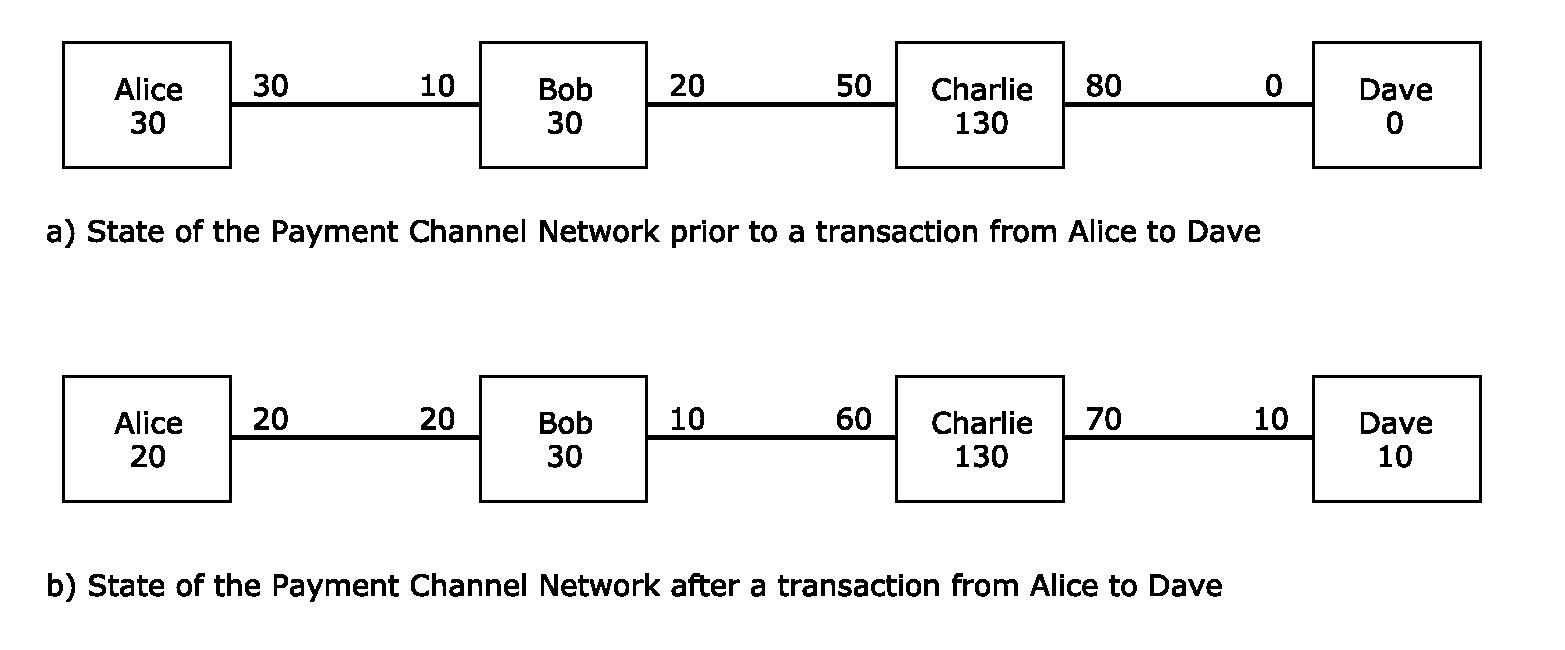
\includegraphics[width=450pt]{Images/PaymentChannelNetwork.pdf}
\caption{Example payment channel network with four participants.}
The lines show the channels and the associated numbers represent the funds of each party in that channel. Alice performs a transaction to send ten units to Dave. Note how the channels adjust their fund associations to reflect the new overall state.
\label{fig:PaymentChannelNetwork}
\end{figure}

\subsection{Cloud Resource Management and Tracing}

Cost analysis and tracing in the cloud is a broad topic and closely relates to the general problem of tracing and analyzing distributed system and how to manage resources in the cloud in general. This highly relates to the goal of this thesis to reach transparency of costs in a microservice based system.\\
Approaches like X-Trace \cite{fonseca2007x} exist since quite a while and Google's Dapper System \cite{Sigelman2010}, which uses sampling and annotates remote procedure calls between services to mark dependencies, proofed to be valuable, such that Open Source implementations like Zipkin \cite{web102} followed its patterns. Amazon provides its own tool inside AWS called AWS X-Ray \cite{web41}. Also newer academic approaches like Pivot Tracing \cite{mace2015pivot} should be mentioned in this context.\\
It is worth noting however, that these systems mostly use tracing to find bugs in the software and to help with troubleshooting problems. Analyzing the dependencies in terms of usage and financial factors is usually not their core objective.\\

Other research focuses on the analysis of costs of cloud deployments \cite{Jennings2015}\cite{Sharma2012} and microservices specifically \cite{Leitner2016}. There are interesting comparison between traditional (monolithic) and novel (serverless) deployments \cite{Villamizar2017}. Scientific models like Costradamus \cite{kuhlenkamp2017costradamus} provide an interesting approach to analyze the costs in a distributed cloud deployment, too.\\
Determining how much a service should charge for its responses is not part of this thesis and prototype. This involves too many factors nethertheless the research above can help to estimate these costs.

\newpage
\section{System Design}

In the following sub-chapters the architecture and concept of the system will be explained. Also an analysis of possible attack vectors, threats and how they are mitigated by the system is included.\\
First, a short naive approach is presented to motivate the final system architecture and to present some of the problems when using blockchain technologies for use cases with high throughput requirements.\\
After the detailed explanation of the state channel based system, some advanced concepts, like possibilities for price differentiation and the tracing of transitive dependencies and payment flows, are described. Likewise, the security aspects of the systems are discussed in detail.

\subsection{Naive Approach}

The payment system is supposed to mitigate the mistrust and fraud problems that can occur in any trade. In such a scenario, both parties do not fully trust each other. Usually an intermediary, that both parties trust, is then used. Examples for such intermediaries are credit card networks like VISA and MasterCard or PayPal for online services. Also, a notary can act as such an intermediary for larger deals.\\

In this blockchain based system the neutral, trusted third party will be a smart contract that is deployed on the blockchain. This means that there is no person or organization involved that needs to be trusted. Both parties can verify the code of the smart contract and only need to trust in the correctness of the blockchain system. A fee is still charged but usually considerably lower than for conventional intermediaries. In the Ethereum network this fee is paid in form of gas based on the amount of storage and computing steps of the smart contract.\\
The properties of the blockchain system guarantee that all transactions are in a specific order and all participating nodes agreed on them. This is important to create a single point of truth of how much funds each party owns.\\

\begin{figure}[H]
\centering
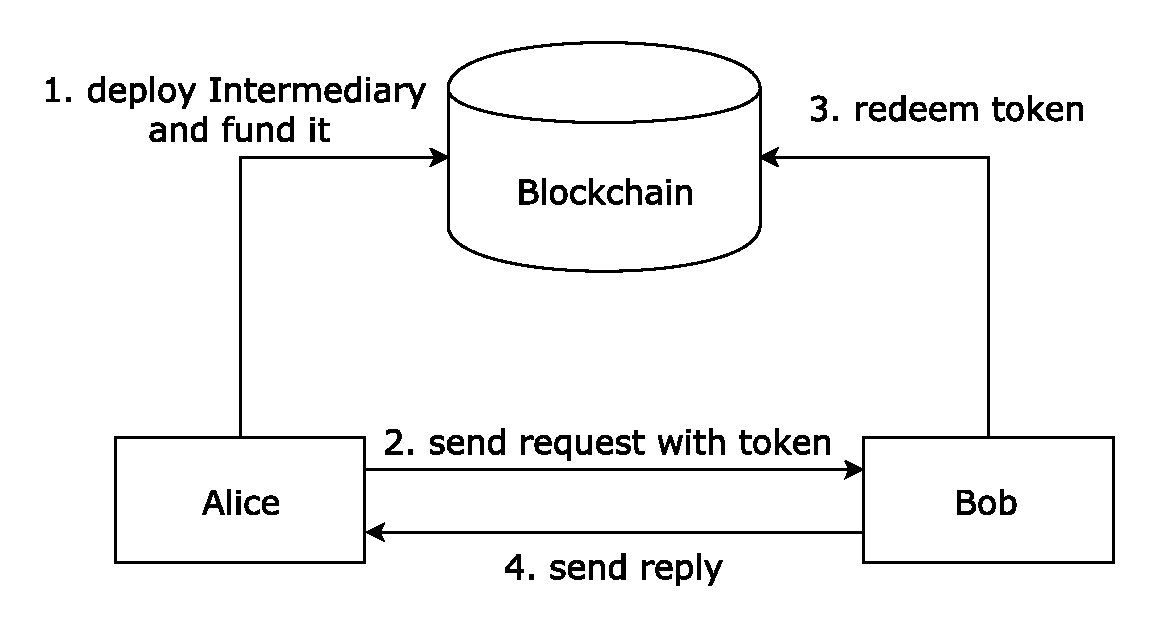
\includegraphics[width=350pt]{Images/NaiveOverview.pdf}
\caption{Naive Approach - Overview.}
\label{fig:NaiveApproach}
\end{figure}

Assuming Alice knows the logical addresses of Bob and the conditions that Bob imposes for its service, Alice can deploy a smart contract - from now on called Intermediary - to the blockchain (step 1 in figure \ref{fig:NaiveApproach}). The logical addresses will usually be the address of Bob's account in the blockchain network and some URI to send a request to Bob - e.g. an REST (Representational State Transfer) \cite{fielding2000representational} API endpoint. The Intermediary is bound to the interaction between Alice and Bob and its parameters cannot be changed later on. Alice can now deposit funds in the Intermediary. Alice will not be able to retrieve these funds until the contract between her and Bob is terminated.\\

Having this setup in place, Alice can start to send requests to Bob. Along the usual request payload, which is needed to fulfill its purpose, a cryptographic token and some metadata will be sent (step 2). The metadata includes who this request sent, the address of the Intermediary and a random nonce that was used to generate the token.\\

The cryptographic token is used to sign the request. The receiving service Bob now sends the token and the metadata to the Intermediary (step 3). The Intermediary verifies the integrity of the token. The Intermediary then internally transfers the cost of one request from the internal account of Alice to the account of Bob. Bob can later on request to transfer its funds from the Intermediary to anywhere else - probably to its own account. The Intermediary also saves the token as redeemed, so that Bob cannot redeem it again.\\

If this validation and transfer was successful, Bob can send its reply to Alice (step 4).\\

To generate and validate the token, asymmetrical cryptography - also known as public key cryptography \cite{salomaa2013public} - is used. This is the same mechanism that a blockchain uses internally.\\
The token used in the payment process is a cryptographic signature and the message data consists of the Intermediary address, the sender address and a nonce. The nonce is a random value that is created by the sender and is required to differentiate different messages. If the signature would only be based on the Intermediary address and the sender, it would be the same for every request. This would defeat its purpose as a "use once token".\\

For private and public keys, the keys and the infrastructure of the blockchain network can be reused. In this system every participant already has its own private and public key pair. Also the implemented cryptographic algorithms can be reused.\\

This system now facilitates a safe and tamper proof automated intermediary.\\
The consumer cannot trick the provider because it has to send a new token for every request. The provider can easily redeem it against the locked funds in the Intermediary. This avoids the "delivered but not paid" case.\\
The provider cannot trick the consumer by charging it for requests that never happened. It cannot redeem a token twice and a valid token must be created by the consumer. This avoids the "charge too often" case.\\

This naive approach would now create one transaction on the blockchain for each request. Also for each request a new token must be stored in the smart contract. This leads to two problems: high costs and large delays.\\

A usual blockchain transaction in the Ethereum networks takes about 15-20 seconds \cite{web12}. This is too slow for usual microservice interactions where response times in the range of tens of milliseconds are desired.\\
Each transaction incurs a transaction fee, currently about 1 USD \cite{web11} in the Ethereum network. This means that the value of a request might already cost more transaction fees than it is worth.\\
Storing tokens on the blockchain in the smart contract also incurs a fee. For thousands of requests per day this incurs an unmanageable amount of storage and therefore consumes a tremendous amount of funds.\\

This means a way needs to be found to scale this system and avoid making so many transactions on the blockchain without decreasing the de facto security of the system.\\

Beyond this problem, in this naive approach each party also needs to run a blockchain node to submit transactions. Because of the size of the blockchain and the required computing power, it is no option to run a dedicated blockchain node alongside each microservice on the same host. A solution needs to be found, such that microservices can use this system without too much management and configuration effort. Also the generated computing overhead on the microservice itself should be limited.\\


\subsection{State Channel Approach}

\subsubsection{High Level Overview}

The final system is similar to the initially described naive approach. To address the problems with the naive approach, two essential modifications to the system will be made.

\begin{itemize}
\item To avoid making too many real blockchain transaction, the system will use a state channel approach.
\item To address the complexity and performance requirements for the interaction with the blockchain, a proxy server for the payments will be introduced. It will be called Payment Server from now on.
\end{itemize}

\begin{figure}[H]
\centering
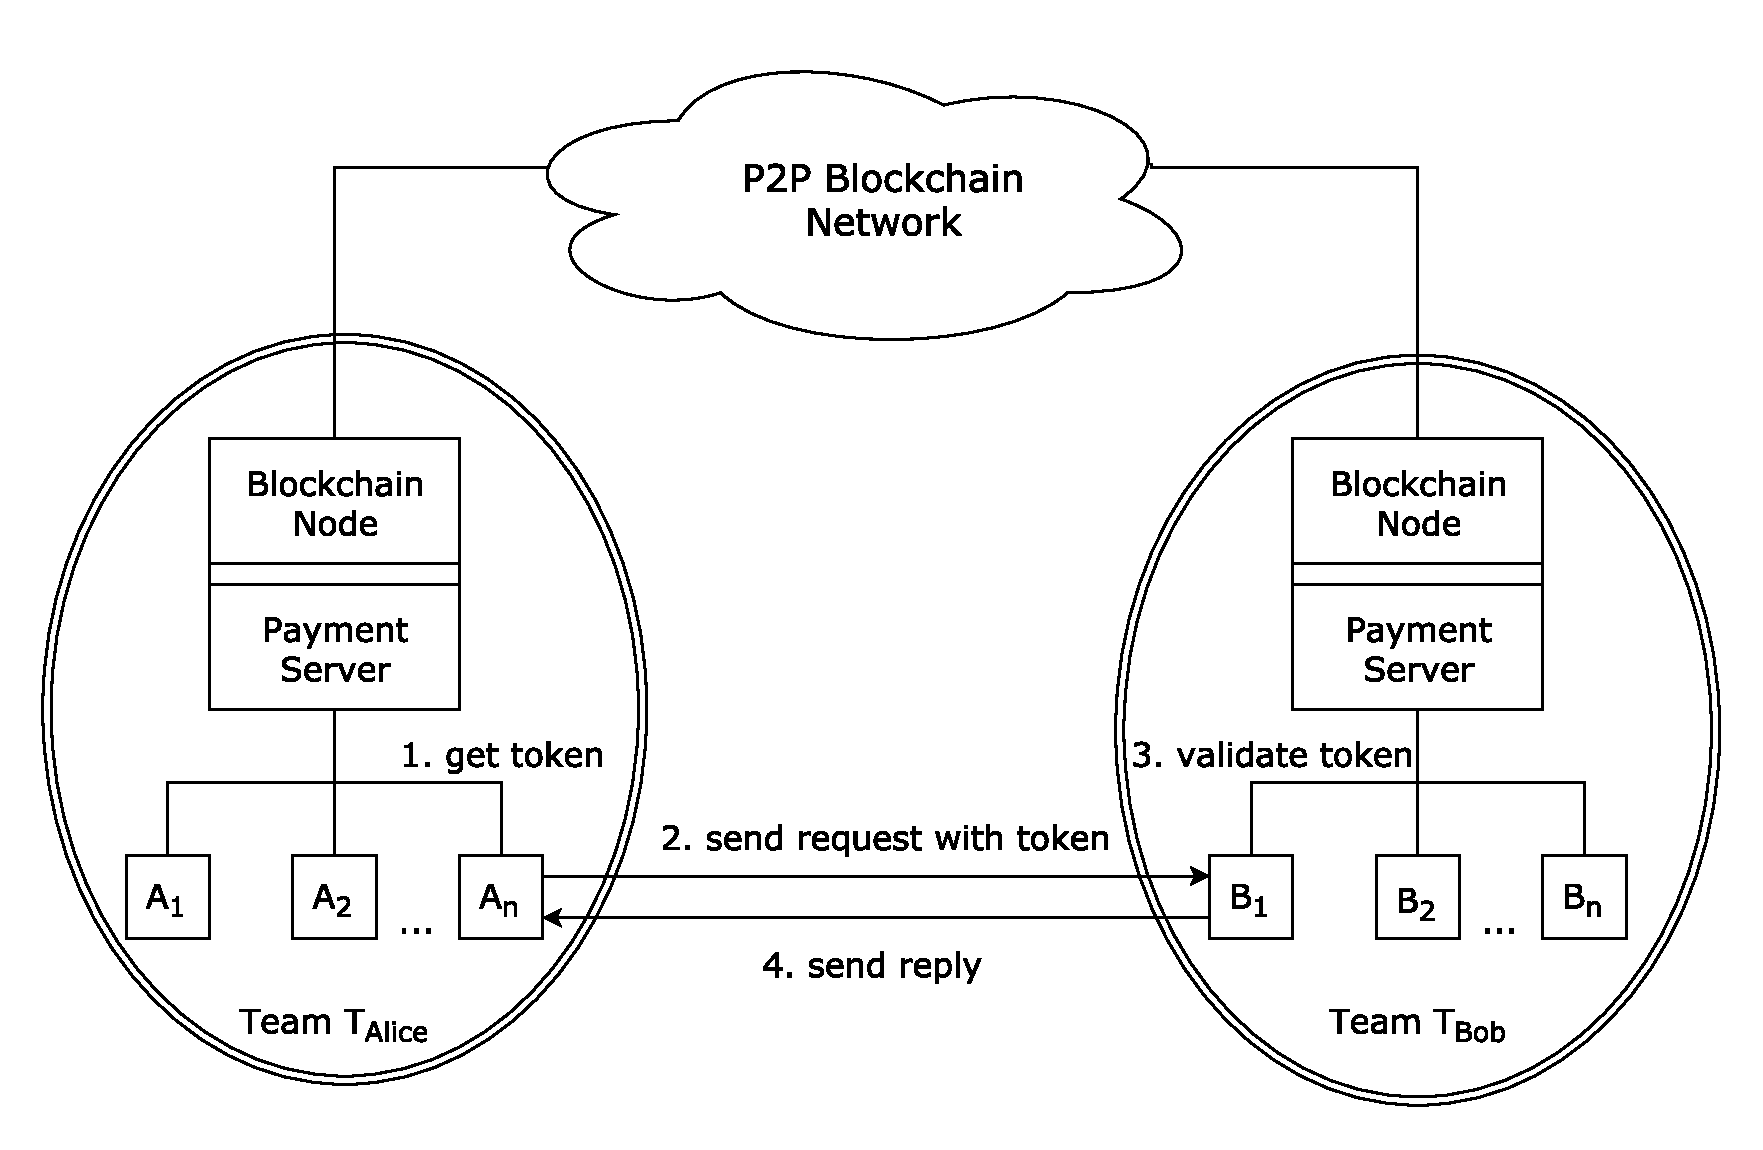
\includegraphics[width=450pt]{Images/HighLevelOverview.pdf}
\caption{High level architecture overview of the proposed system.}
\label{fig:HighLevelOverview}
\end{figure}

Figure \ref{fig:HighLevelOverview} shows a high-level overview of the system for the case of two replicated services named Alice - with its instances $A_1$ to $A_n$ - and Bob - with its instances $B_1$ to $B_n$. These services are run by two different teams, $T_{Alice}$ and $T_{Bob}$. Each team runs one Payment Server instance and one blockchain node. The blockchain nodes of all teams are connected in a peer-to-peer blockchain network. They sync their state and transactions based on the consensus algorithm. The Payment Server of each team interacts with the blockchain node on the one side and the individual service instances on the other side. It never interacts with another Payment Server. The service instances of Alice communicate with the service instances of Bob.\\

The Payment Server performs the complex transaction parts for its clients. To recap from earlier, every request that is send from one service to another needs to include a token. This token then also needs to be validated on the receiving side, which is the main responsibility of the Payment Server. The service instances trust the Payment Server and delegate the token generation and validation to it. Through this the clients can stay mostly dumb, do not need to interact with the blockchain themselves and do not need to persist state.\\
Beside these responsibilities, the Payment Server also performs the initial Intermediary setup and the contract termination handling. It also keeps certain state information and performs timer-based checks. Both will be discussed later on.\\

The token mechanism from the naive approach is replaced by a multipart token. A token $T$ is now a tuple of multiple values.\\

$\mathbf{T = (T_{ID}, R, I, C, S)}$\\

It consists of a token ID $T_{ID}$, which will be reused for multiple requests, a request counter $R$, the address $I$ of the Intermediary on the blockchain, the address $C$ of the consuming service, and a cryptographic signature $S$, which was generated by the consuming service with its private key over the other four values.\\

A token is now unique only by its combination of token ID $T_{ID}$ and request counter $R$. Every time Alice sends a request to Bob she will increase the request counter of the token by one. The token ID is reused for multiple requests. Each token is superseded by a token with the same ID but a higher request count.\\
Bob now does not need to redeem each individual token but only needs to track the latest one. He can eventually redeem the latest token - the one with the highest request count - at the Intermediary and receive a payment for the number of requests on that token. Other tokens with the same ID but another request counter cannot be redeemed. The Intermediary invalidates the token ID after a redemption and issues a new token ID for future requests.\\

The new flow for a request will be:

\begin{itemize}
\item[] 1.) $A_x$ gets a token with the latest request count from its Payment Server.
\item[] 2.) $A_x$ sends the request to Bob.
\item[] 3.) $B_y$ receives the request and validates it via its Payment Server.
\item[] 4.) Bob's Payment Server saves the token and the request count.
\item[] 5.) $B_y$ sends the response to $A_x$ if all validations pass.
\end{itemize}

Eventually Bob can redeem the token.\\

Overall the system has four Phases that are simplified shown in Figure \ref{fig:Phases}.\\

\begin{figure}[H]
\centering
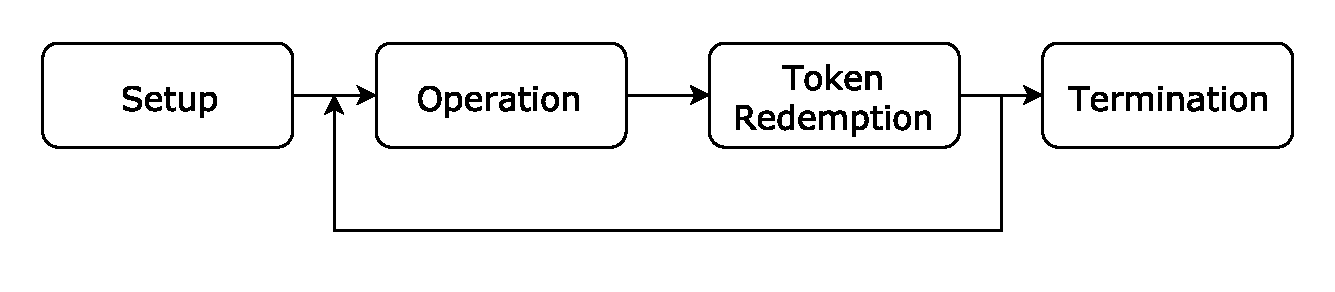
\includegraphics[width=350pt]{Images/Phases.pdf}
\caption{Phases of the proposed system.}
\label{fig:Phases}
\end{figure}

\subsubsection{Setup Phase}

For every relation between two microservices a dedicated Intermediary is required. This needs to be setup once on the blockchain but can then be reused for this relation even after a crash or restart of the microservices.\\
Figure \ref{fig:Setup} shows the sequence of interactions for this process.\\

\begin{figure}[H]
\centering
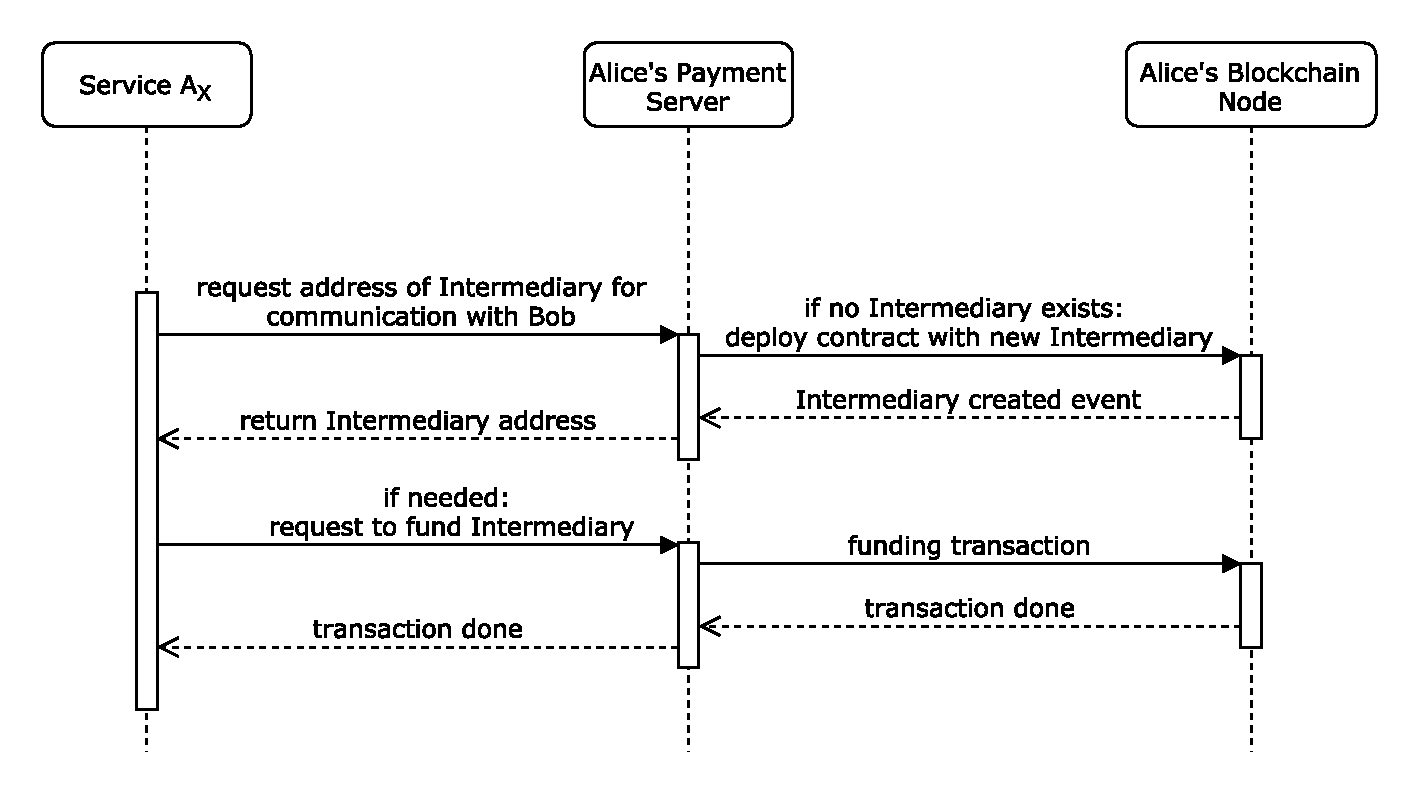
\includegraphics[width=450pt]{Images/Setup.pdf}
\caption{Setup phase of the proposed system.}
\label{fig:Setup}
\end{figure}

When a new service instance $A_x$ is launched, it will contact its Payment Server to get an Intermediary contract for its communication with the other service Bob. The Payment Server will then perform a lookup if an active Intermediary for this relation already exists. If not, it will create one on the blockchain. This creation costs a transaction fee and is paid by the account of the consuming service Alice.\\

When the Intermediary is available, this information will be returned to the service instance $A_x$. It can then request to deposit funds into this Intermediary. It can also configure some auto-funding settings, so that the Payment Server can automatically try to refund the Intermediary in case the funds cross a certain threshold.\\

After this funding transaction is done, the service instance $A_x$ is ready to perform requests against Bob.

\subsubsection{Operation Phase}

The operation phase is the repeated - or even parallel - execution of sending requests from a consuming service Alice to the providing service Bob. Figure \ref{fig:OperationPhase} shows the sequence of events in one of these request-response interactions.\\

\begin{figure}[H]
\centering
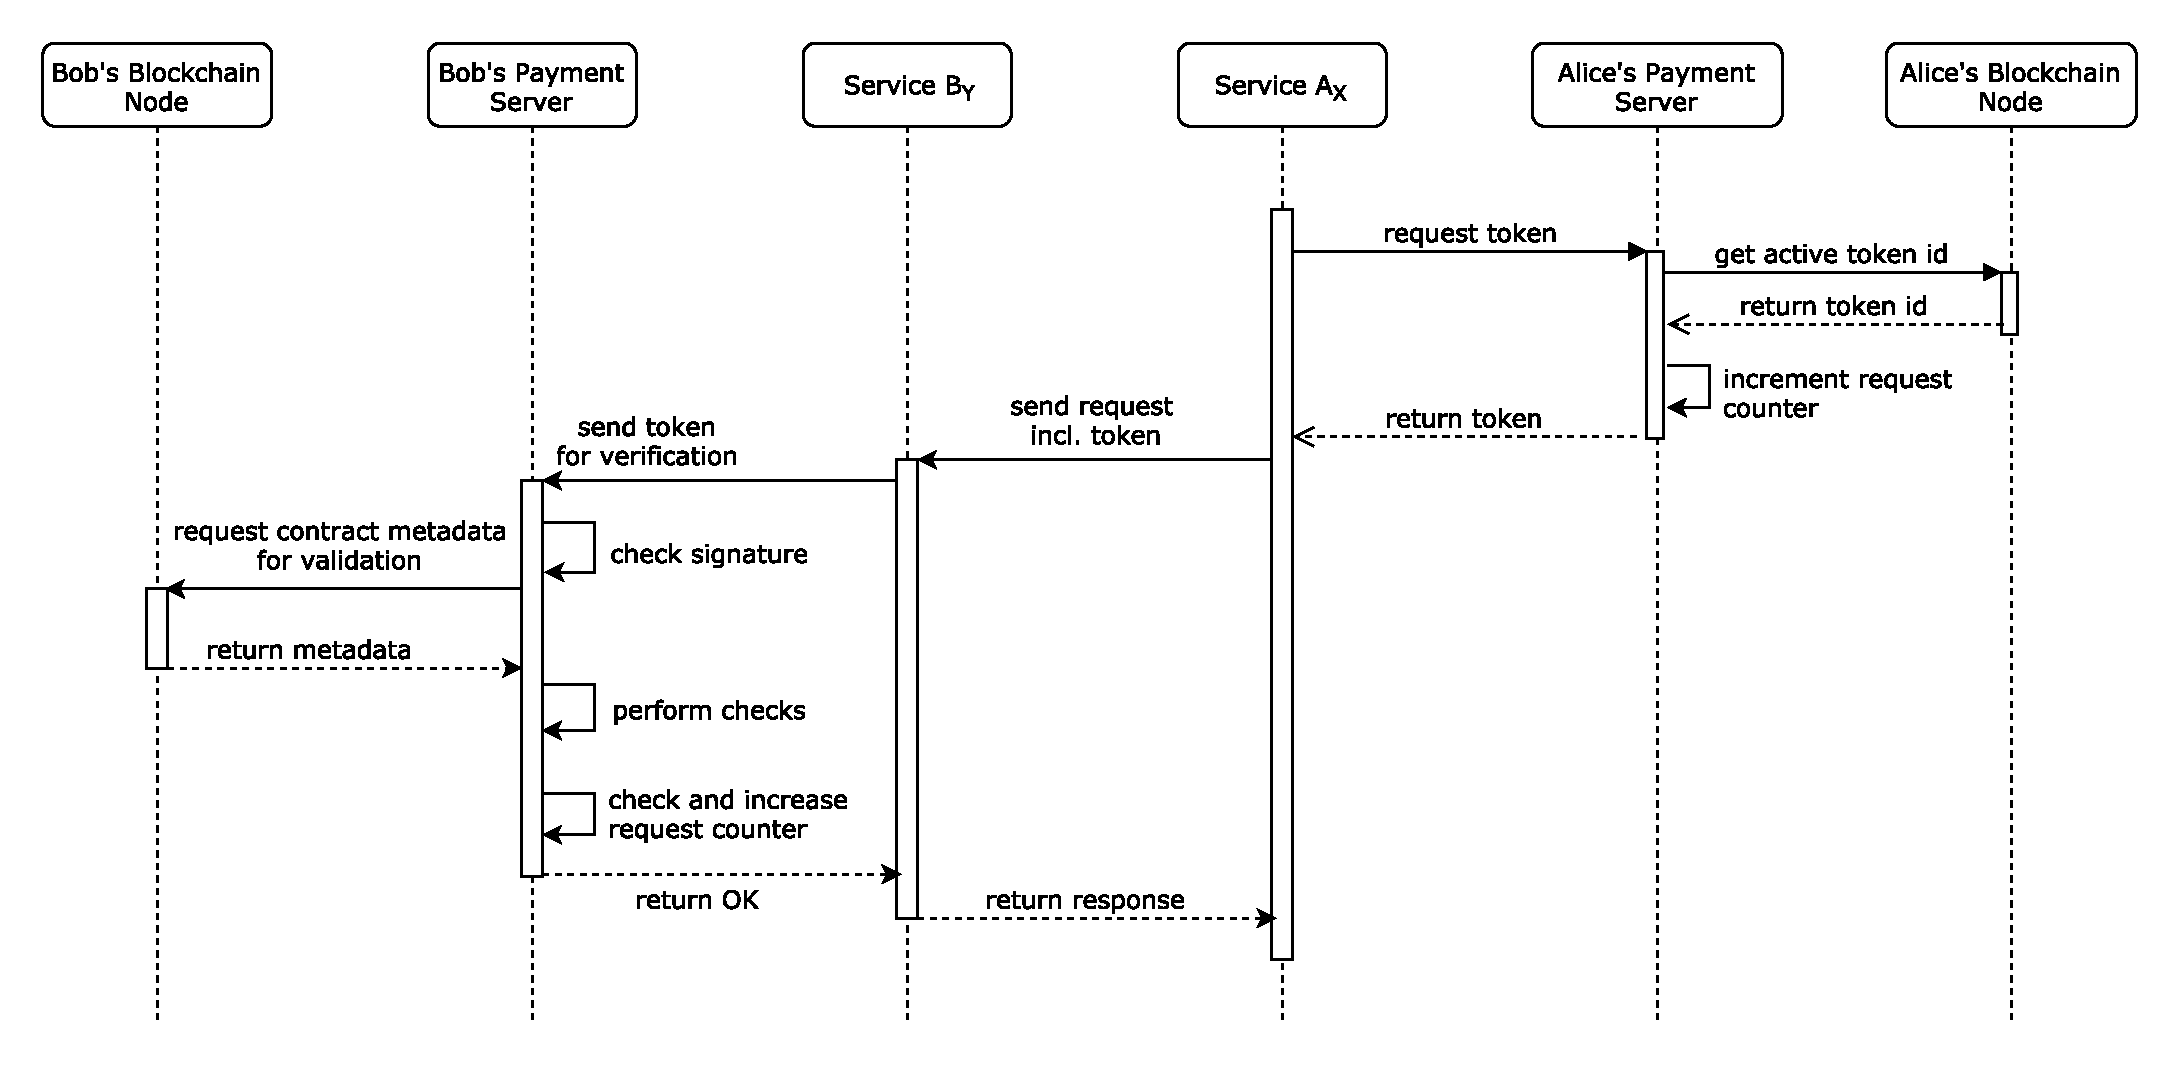
\includegraphics[width=450pt]{Images/OperationPhase.pdf}
\caption{Operation phase of the proposed system.}
\label{fig:OperationPhase}
\end{figure}

Assuming $A_X$ wants to perform a request it first requests a token from its Payment Server. As outlined above, the token consists of the ID of the token $T_{ID}$, the current request count $R$, the blockchain address $I$ of the Intermediary, the blockchain address $C$ of the sender and a cryptographic signature over these values. The ID of the token is reused for multiple requests until the receiving side redeems the token. This invalidates the token ID for further use. The currently active token ID is stored in the Intermediary on the blockchain. That is why the Payment Server will get the latest token ID from its blockchain node.\\
After getting the token ID, the Payment Server will increment its internal request counter by one. If the token ID changed it will reset the counter to zero first. Note that this request counter increment and get operation is an atomic operation to avoid race conditions. Each request number can only occur once.\\
The incremented request counter, all the other metadata and the signature will then be returned to the service instance $A_x$. It can then send this alongside the other request payload to the providing service Bob.\\

The service instance $B_y$ that received that request will forward this metadata to its Payment Server for verification.\\
This Payment Server will first validate the token for integrity using the asymmetric cryptographic mechanisms.\\

After this, it needs to check the metadata and the state of the Intermediary.

\begin{itemize}
\item First of all, the Intermediary should not have been terminated yet.
\item The parameters encoded in the Intermediary should also match the requirements of the providing service. This especially includes the cost per request, but also parameters like timeout durations. This check needs to be performed only once per Intermediary and the result can be cached by the Payment Server because this data is stored immutable in the Intermediary.
\item The received token ID must also be verified if it is still active and valid.
\item The Payment Server also needs to check if the funds of the consuming service that are locked inside the Intermediary are large enough to cover the value of the token. So the number of requests on the token times the cost per request must be less than the funds in the Intermediary.
\item Lastly the request count must be validated. This needs to be an atomic check and update operation to avoid race conditions between multiple requests that are validated at the same time.
\end{itemize}

The naive approach of the request count validation would be to just check whether the received new counter is greater than the previous stored one. Although the requests are generated on the consuming service side in a serialized way - the counter there is atomic - the requests may not reach the providing service in that order. This means, that the request with count ten might arrive before the request with count eight. In a naive approach, request eight would be declined now, although it was not answered before.\\
To avoid this problem, the Payment Server not only tracks the largest received request count, but also keeps a list of all request counts below this value that were not yet received.\\

If all those checks passed, $B_y$ can send its response to $A_x$ and the interaction is done.\\

Opposed to the flow with a direct token redemption, this flow does not perform any transactions on the blockchain. It only performs cheap read operations. These read only operations happen locally on the blockchain node and do not require any interaction with the rest of the blockchain network. Opposed to transactions, they do not incur a transaction fee and have comparatively short latencies.

\subsubsection{Token Redemption}

Bob can at any time decide to redeem the active token. However, this should not happen too often but regularly enough to reduce the impact of losing the token through a server crash or similar incidents. To redeem a token a blockchain transaction is required. This might take several seconds - depending on the blockchain's performance. The usual operation of signing and validating requests between the services needs to continue during this period.\\
Therefore, the token redemption is split into two transactions, as shown in figure \ref{fig:TokenRedemption}. First, the providing service Bob, that wants to redeem the token, performs an announcement transaction. With this a new token ID is generated and set as the active one. The existing token ID is marked as soon expiring. The duration of the tolerance period during which tokens with the old token ID are still valid, is specified immutable in the Intermediary during the setup.\\

\begin{figure}[H]
\centering
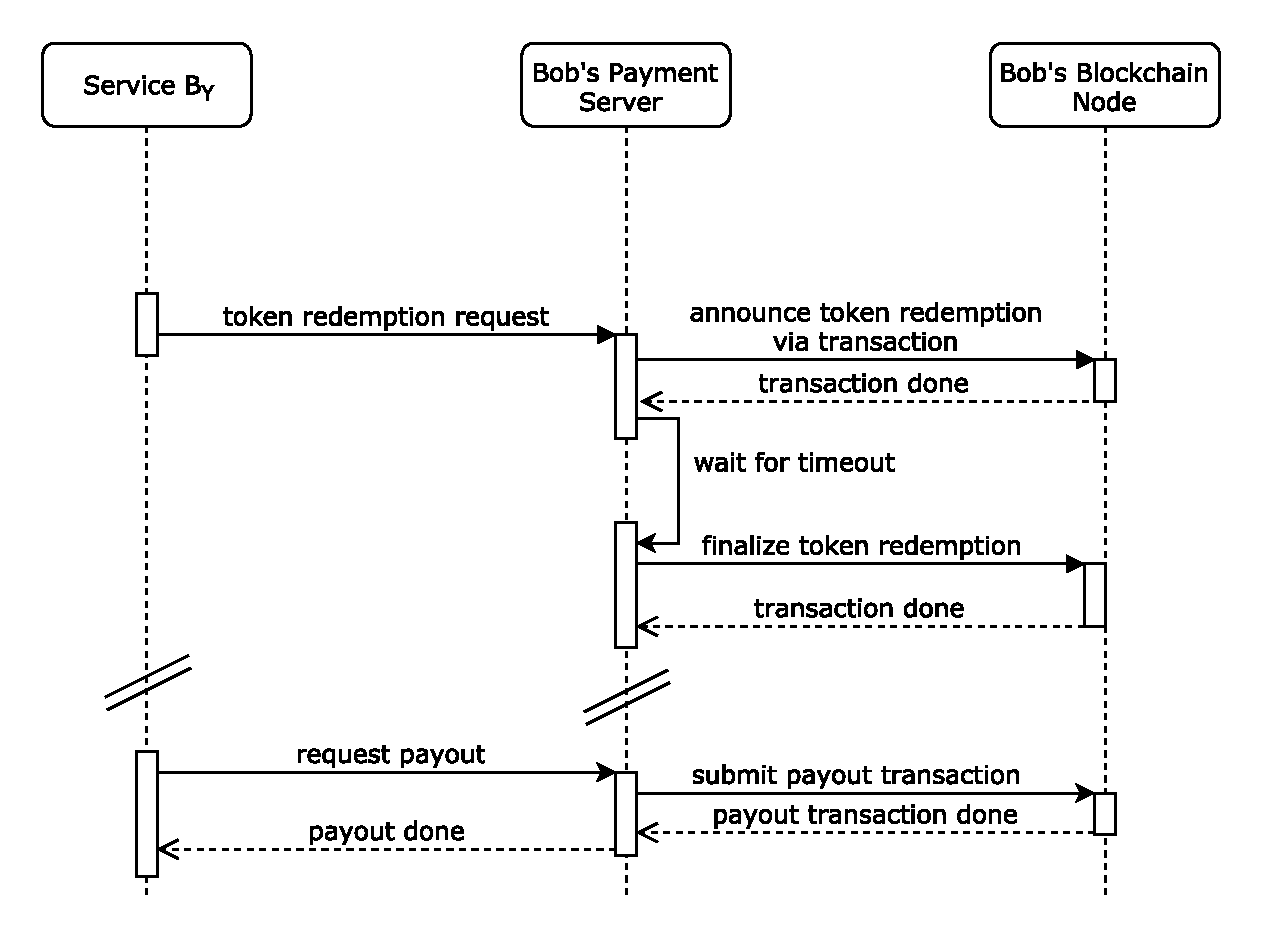
\includegraphics[width=450pt]{Images/TokenRedemption.pdf}
\caption{Token redemption flow in the proposed system.}
\label{fig:TokenRedemption}
\end{figure}

After this transaction is completed, any new request that the consuming service Alice signs will include the new token ID. Requests that were still on the way can still be validated by the providing service Bob during the tolerance period.\\

When the tolerance period is over, Bob will deny requests with tokens with the old token ID. It is then Alice's fault if the outdated token ID is still used. Bob can now take the latest token with the now expired token ID and request count and redeem it at the Intermediary. This is the second transaction. The Intermediary now marks the old token ID as redeemed. The funds inside the Intermediary will be transferred from Alice to Bob according to the number of requests and the cost per request.\\
Note that this transaction does not happen automatically, it needs to be triggered explicitly. In the current system, the Payment Server runs a timer to perform the second transaction after the tolerance period. The second transaction is protected against too early invocation.\\

As the providing service, Bob has the privilege to withdraw its funds from the Intermediary at any time. This is possible because the Intermediary represents a one-way flow of payments.\\

It should be noted, that it is not possible to start another token redemption while a token redemption is still in progress. This would increase the complexity unnecessarily.\\

The duration of the token redemption tolerance period should be chosen with care. It needs to be larger than the time required to complete the initial transactions and to propagate it to all nodes in the network, plus the round trip time of the slowest request send by the consuming service Alice. An additional tolerance is recommended as well.\\
For now, it is recommended to set it to about 60 seconds for a normal HTTP REST API backed by an Ethereum network with average block mining times of 15 to 20 seconds.\\
Please note that this timeout is related to the termination timeout discussed in the next section and should be significantly shorter than it.

\subsubsection{Termination Phase}

Every relationship might come eventually to an end. For this case, a structured shutdown of the Intermediary is required.\\

In case the providing service wants to shut down the service, it is a straightforward process. It can just stop accepting new requests, redeem its last token and send a shutdown transaction to the Intermediary. The Intermediary can then instantly shut itself down and pay out the locked funds to both parties.\\
If Bob shuts down the Intermediary before redeeming his last token it is his fault. He had the full control over the process.\\
Alice cannot do anything about this shutdown but also does not lose any funds in the process. However, Bob should let Alice know that it will terminate the relationship to avoid unnecessary requests and let Alice prepare for this situation but this is not required and not part of the prototype.\\

If the consuming service Alice wants to terminate the relationship the process is more complicated. Bob might still have a token that he wants to redeem before the system is terminated.\\
To solve this, the termination by Alice is performed - similar to the token redemption - through two transactions and a tolerance period. The first transaction announces the upcoming termination through a state variable in the Intermediary. Through this the providing service - or more its Payment Server - can determine the expected termination time of the Intermediary. The Payment Server of the providing service Bob needs to check for such a termination regularly, either on every incoming request - might not be enough since requests may happen infrequently - or via an interval timer.\\
When Bob detects the termination, it should stop accepting requests and start a final token redemption process to redeem the last token.\\
After the last token has been redeemed, Bob can terminate the Intermediary itself or wait for Alice to perform the second, terminating transaction. This will payout the funds to both parties based on the latest state in the Intermediary.\\
If Bob does not redeem its final token in time, it is considered to be his fault, since he had enough time to do so.\\

The termination timeout duration should be chosen very carefully. It is better to have a longer timeout than a shorter one. A termination is supposed to be a very rare transaction and therefore performance is not that important.\\
The timeout needs to be longer than it takes to perform a token redemption. So it must be significantly larger than the token redemption tolerance period. It also needs to account for the time that the providing service Bob might need to detect the termination. This detection can be implemented with a recurring timer. It should be considered that - for whatever reason - the providing service Bob and its Payment Server might not be able to communicate with the rest of the network for a certain amount of time. This can happen e.g. because of network or server failures.\\

Based on these criteria it is for now recommended to have a termination timeout of at least 15 minutes and check once every minute for terminations.\\

This timeout mechanism for the termination is a variation of the "Challenge Response Pattern"  \cite{eberhardt2017or} described earlier. The consuming service "challenges" by submitting a termination request. The providing service can then "respond" by submitting its last token.\\

\subsection{Price Differentiation}

So far, a fixed pricing per request per service was assumed in this system design. In reality, however, a more differentiated pricing might be desirable. The pricing could be adjusted in a variety of ways:

\begin{itemize}
\item[] P1) Individual prices for different clients.
\item[] P2) Different prices based on the time of day or load on the system.
\item[] P3) Different prices based on the size or complexity of a request.
\end{itemize}

It is common business practice in the business-to-business sector that different clients might get different prices based on their individual negotiations (P1). Usually these agreements are also kept private, a property which is not possible in this blockchain based system since any member of the network can read all the data.\\
Negotiating individual prices is easily possible within the system. The price is part of the contract and set by the consuming service, when deploying the Intermediary contract. The providing service then needs to accept the conditions. Both services can communicate prior to this deployment to negotiate a price that fits both. This could either happen automatically or via human interaction.\\

Changing the price after deployment is a more complex task (P2). A service provider might want to give an incentive to consumers to use the service during a time when the load on the system is low. This can be especially relevant in cloud computing settings where resources can be allocated dynamically and cloud providers also offer resources with dynamic pricing - e.g. Amazon's Spot Instances \cite{web96}.\\
However, both parties must agree to the price first. In the current setup, it is fixed upfront and stored in the contract. This makes it not easily changeable.\\
One solution to this is to not encode the price in the contract at all and to price each request individually. Instead of having a request counter associated with the token, the total price of all performed request summed up is used. One disadvantage of this approach is that it requires additional communication to negotiate the price for each request. Another one is that the number of requests that where performed at a certain price cannot be inferred anymore.\\
Another solution to the problem is to attach the price change to a token redemption as seen in figure \ref{fig:DynamicPricing}. The provider can redeem a token and at the same time set a new price per request for the next token. Through this, the consumer has enough time to adjust to the new pricing and can decline it by not using the service anymore. The number of requests and their price is still traceable since it is bound to a specific token which will be submitted to the blockchain eventually. The disadvantage of this approach is that a price change is bound to the timeout and transition intervals of a token redemption.\\

\begin{figure}[H]
\centering
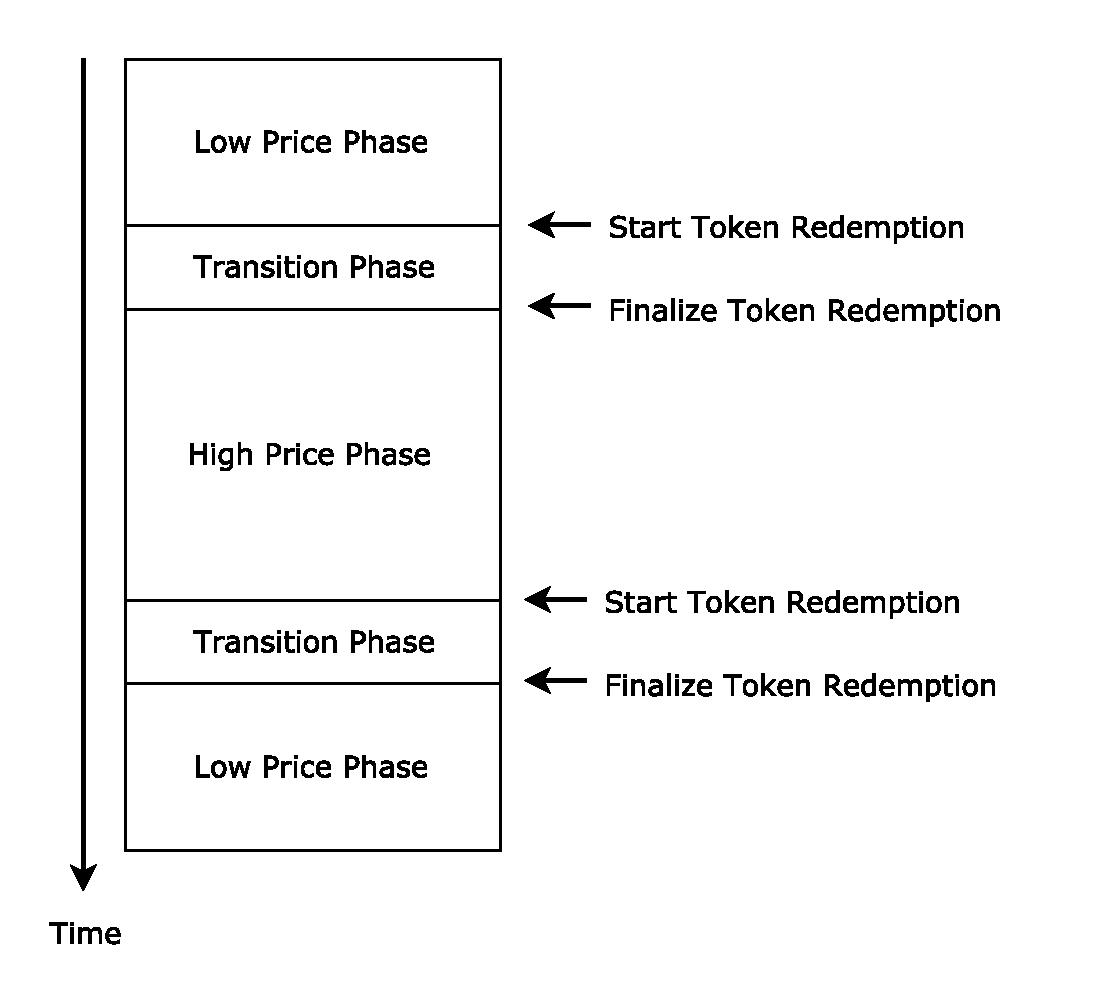
\includegraphics[width=400pt]{Images/DynamicPricing.pdf}
\caption{Change of the per request price can be performed during a token redemption.}
\label{fig:DynamicPricing}
\end{figure}

Adjusting the price of a request based on its size or complexity (P3) is a reasonable use-case, too. Imagine a service that processes texts and delivers the result of some linguistic processing about it. Of course, this service should be able to charge more for a large text than for a short paragraph.\\
As discussed for (P2), this problem can be solved by using the total price of all requests instead of a request counter in the token, but it also faces the same problems.\\
On the other hand, it is possible to categorize each request into a limited set of categories. Each category has a dedicated price and a dedicated request counter. Storing this pricing table does only consume limited space in the Intermediary contract and the request counters can still be encoded in the token. After redeeming the token, the information about how many requests of which category were made is stored in the blockchain and can be used for analytics.\\

If the business needs require it, it is possible to combine all three dynamic pricing models to create a service that is able to charge different prices based on consumer, time of day, load of the system and request size and complexity.

\subsection{Transitive Dependency Tracing}

With the proposed system it is now possible to track the exchange between every two parties in a microservice ecosystem. However, it is not possible to track transitive dependencies.\\

\begin{figure}[H]
\centering
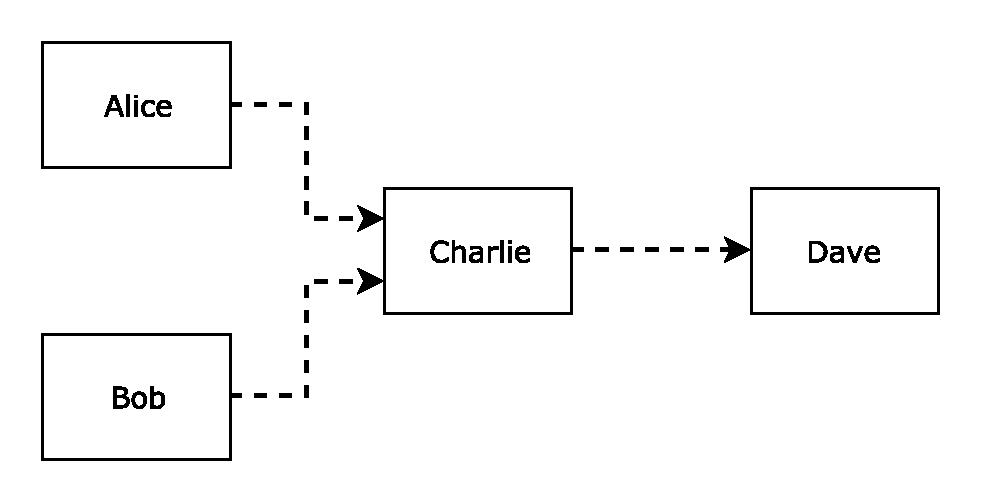
\includegraphics[width=250pt]{Images/TransitivityBefore.pdf}
\caption{Setup of four services with transitive dependencies.}
\label{fig:TransitivityBefore}
\end{figure}

Assume four parties Alice, Bob, Charlie und Dave which each represent a service - like shown in figure \ref{fig:TransitivityBefore}. Alice and Bob are public end-consumer-facing services and use Charlie to provide them with some data. Charlie itself uses Dave only for some requests from Alice and Bob to deliver the requested response.\\
From the intermediary contracts between Alice and Charlie, as well as between Bob and Charlie, it is easy to infer who used Charlie how much. It is also directly possible to infer the usage of Dave by Charlie. But since Alice's and Bob's requests to Charlie might not always trigger a request from Charlie to Dave, it is unknown how much of the load was generated by Alice and how much by Bob.\\

\begin{figure}[H]
\centering
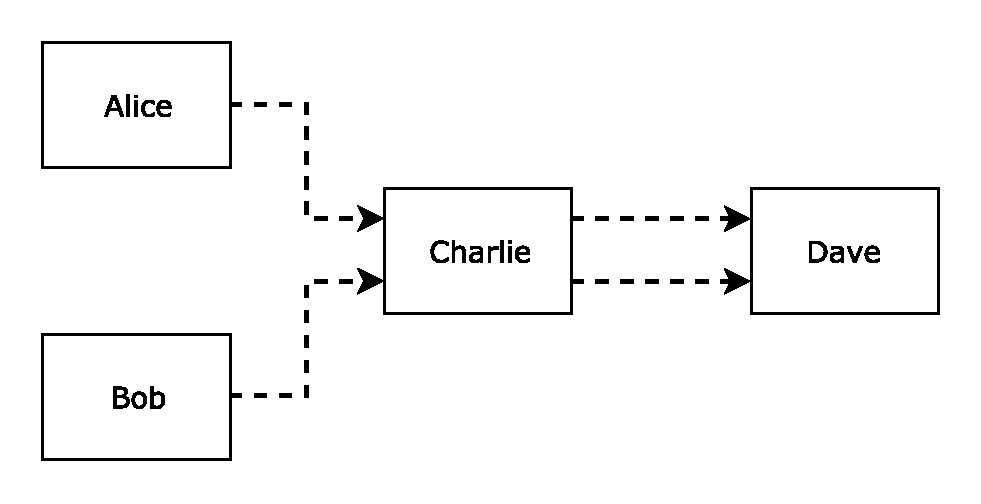
\includegraphics[width=250pt]{Images/TransitivityAfter.pdf}
\caption{Setup of four services with transitive dependencies made traceable by dedicated payment channels between Charlie and Dave.}
\label{fig:TransitivityAfter}
\end{figure}

For systems with a small number of transitive dependencies and short dependency chains two simple approaches to the problem seem viable.\\
Charlie could create a dedicated Intermediary contract to Dave for each of his consumers - see figure \ref{fig:TransitivityAfter}. These contracts would independently track the usage of Dave caused by Alice and Bob.\\
Or Charlie could create a contract with multiple requests counts, one for each consumer. This would be a similar solution as to the dynamic pricing case (P3), where a pricing table assigns different prices based on the type of the request.\\

These approaches face problems in terms of scalability for longer transitive dependency chains or complex networks. The number of mapping table entries or deployed contracts would grow significantly.\\
Additionally, it would be easy for a service like Charlie to manipulate the statistics by serving requests from Alice under the name of Bob to Dave. Employing a cryptographic security mechanism here might not be feasible since the usage of Dave should be an implementation detail of Charlie which is not required to be revealed to Alice and Bob but only to auditing instances. It is also questionable, if Charlie would have a motivation to manipulate the distribution, as long as he has no financial advantage from it.

\subsection{Security Considerations}

Since the system tracks sensitive values it is a system attractive to attack. This was considered throughout the design of the system. It is also one of the reasons why blockchain technologies were chosen for it. In the following, some attack and manipulation scenarios are described and evaluated.\\

A consuming service could try to trick the providing service by trying to \textbf{double spend} its funds. This cannot happen in this system. First of all are the funds of the consuming service locked in the Intermediary. As long as the Intermediary is active they cannot be spent on something else than this service interaction. The consuming service could still send two requests with an identical request counter. The providing service would detect this because it keeps track of the request counter and denies repeated requests with the same count.\\

On the other hand, the providing service might want to trick the consuming service by trying to \textbf{redeem a token twice}. This cannot happen since the Intermediary contract keeps track of the token IDs and only accepts a token once. The token is cryptographically signed and therefore cannot be generated by someone else than the consuming service.\\

The Payment Server of each team is a crucial point in the system. It needs access to the private keys for its services and a connection to the blockchain node. It also keeps relevant internal state like the request counts. \textbf{A hacker could try to attack a Payment Server}. One cannot totally avoid this scenario. However, it has a limited impact - only on the services and service relationships managed by that Payment Server. The Payment Server should also not be publicly accessible. Neither its API nor its management interface. There is no need to expose its API to anyone else than the microservices that are using it. Beside this, the usual security recommendations for the administration of any webserver also apply for this server.\\

The Payment Server of a providing service might \textbf{lose a token}. The reason for it is not important here, but software errors, memory corruptions or other errors are always possible. This loss would only be local. The lost value for the providing service is limited to the number of requests that this token was worth. An older token with the same token ID might still be present or recoverable. The loss in such a situation can be limited by a more frequent redemption of tokens.\\

\textbf{Servers crash or might be unavailable for a certain period of time}, so can the Payment Server. This might cause an unavailability of the system. If, while the Payment Server is unavailable, a termination of a service relationship is started, the Payment Server might not notice this. This is critical if the Payment Server represents the providing side of the relationship and has an unredeemed token. In the worst case, the Payment Server might not be able to recover before the termination timeout is over. Again, the loss is local and limited to the value of the token. All other funds in the Intermediary will still be paid out correctly. The risk for this case can be limited by choosing a large termination timeout that covers a usual recovery duration. Also a frequent token redemption reduces the maximum value that can be lost with the token. Also running a redundant setup of multiple servers reduces the risk of all of them crashing at once.\\

An attacker that controls the majority of the blockchain network is able to rewrite its state by manipulating the majority of the nodes. He would therefore be able to change the Intermediary state or any transaction. This \textbf{51 \% attack} \cite{web27} is a well-known threat in the blockchain community. In practice, it is not a real problem because of the large amount of nodes in public networks. In private networks the situation is different since the amount of nodes is comparatively limited. A blockchain node could still perform its own integrity checks on the state of the chain and detect such an attack but cannot stop it. It is only possible actions are to alarm administrators and to stop the operation of its own services.\\

The consuming service is responsible for deploying the Intermediary contract to the blockchain. A malicious consuming service could deploy a \textbf{modified version of the Intermediary contract} and exploit the providing service through it. To guard against this, the providing service should check the integrity of the deployed Intermediary contract code. The prototype currently does not perform this check to simplify the implementation.\\

The consuming service is intentionally responsible for the contract deployment. Otherwise a malicious attacker could try to drain the funds of the providing service through \textbf{repeated unused Intermediary deployment requests}. For each Intermediary deployment a transaction fee is charged. If the consumer is charged for this cost, it is more likely that he uses that connection responsibly.\\

An attacker could try to perform any form of a \textbf{distributed denial of service attack} \cite{lau2000distributed} against public endpoints that use this system internally for further communication. Since the Payment Server is currently a potential bottleneck of the system it might fail first. The attacker could then try to exploit this circumstance - e.g. through triggering an Intermediary termination while the Payment Server is down. There are no special safeguards against this attack type in the current system. It needs to be protected against such attacks like any public facing web service.\\

A \textbf{man in the middle attack} \cite{desmedt2011man} could try to intercept requests between services and record or even manipulate them. A manipulation of the payment relevant metadata would be detected because all of it is covered by the signature. An attacker can still read the data. However, the data alone is not sensitive. If the attacker has access to the blockchain it is or will be accessible there anyways. One can further protect against this attack by relying on secure connections via TLS \cite{dierks1999rfc}. This should happen anyways to protect the actual request payload. In the current prototype the payment metadata is sent via HTTP header fields. These are not covered by a TLS encryption.\\
Another man in the middle attack vector is the connection between microservice and its Payment Server. This connection is more critical, because an attacker could create consistent fake signatures against a mocked Intermediary. The lightweight microservice client does not - or even cannot - check the provided signature and address from its Payment Server. It must fully trust it. A secure connection is therefore required. Note that in this case the relevant data is not transferred in header fields.\\

If an attacker has access to the REST API of the Payment Server, he might try to \textbf{act as a service} and request tokens on its behalf. This is not possible since all requests from a client to the Payment Server are secured with a signature over the payload. This signature is created with the private key of the microservice. Through this the Payment Server can verify the identity of the service.\\

If the \textbf{private key of any party is lost or leaked}, all of its relationships and funds are in danger. This is as dangerous and unavoidable as in any public-private-key system. In case of a detected leakage, the private key needs to be replaced with a new pair as fast as possible. All connections need to be reconfigured and funds should be moved to secure accounts. Currently, this system does not provide an automated way to do this. This can, for example, be done by forking the blockchain network and reinitializing all service connections. It is also possible to implement a regular key change to reduce the risk of a leakage.\\
At the moment, the microservices and the Payment Server that acts as their delegate need to know the private key. The Payment Server needs it to perform the blockchain transactions and the microservice instances need it to authorize against the Payment Server. The risk could be reduced by using different keys and a mapping table inside the Payment Server for the different use cases. Then a leaked microservice key would not compromise the key for the blockchain access and vice versa. For simplicity reasons, this was not implemented in the prototype.\\

It should be noted that this system does only provide a trustless interaction for the payment part. A service still needs to \textbf{trust the other that it delivers a correct result} and treats the transferred data as expected. One could argue that this creates a slightly strange situation: The two parties do NOT trust each other fully regarding payments but DO trust each other to perform and deliver the right thing.\\

As one might have noticed earlier, the Intermediary contract does \textbf{not completely act like a traditional intermediary}. It only secures the payment side but not the delivery side.\\
A consuming service can send a request with a token to a providing service. When this providing service acts maliciously and does not return a useful response, although the token is valid, the consuming service cannot do anything about this. The Intermediary does not know, whether a valid delivery actually took place. The consuming service can only hope that its next request will be answered or try to resend the request with the same request counter, in case it really just got lost. If the providing service continues to deny a response the consuming service is eventually forced to stop the interaction and alarm an administrator. The value of the send tokens however is potentially lost.\\
This is a case that the current system cannot avoid. The Intermediary has no way to control or check the delivery of the response. One could assume that an alternative solution would be to deliver the response through the blockchain. In this model, the consumer would deposit some funds, then the provider would deposit its answer in an escrow contract, too. This contract now has both and hands the response to the consumer and the funds to the provider.\\
This approach has four problems. First of all the storage on the blockchain is limited. So storing the full response might exceed the limit. Secondly this interaction requires at least two transactions which cost a transaction fee and are slow. Even the fact that the Intermediary does now know that an answer was provided he cannot validate it. The provider might just have submitted some garbage data. As soon as the data is inside the Intermediary it is also readable by anyone. This might violate privacy, although this can be solved by encrypting the data, and the consumer will be able to read the data. It now does not make sense to let the consumer validate the data and possibly reject it as invalid. He could just reject it, even if it is valid because he was already able to completely read it.\\
This approach would add little safety but for a huge cost in terms of time and transaction cost. Also many classic intermediaries or payment networks (e.g. credit card networks) do not act as "full" intermediaries and do not perform the exchange of the delivered value through themselves. For now this risk is considered acceptable.


\newpage
\section{System Implementation}

In this chapter the implemented prototype is explained. The code for it can be found on GitHub (\url{https://github.com/FGoessler/master-thesis}). First the general technology stack is explained, then the specific test scenario is described before some more technically interesting details of the prototype are shown. In particular, some code samples from the Intermediary contract code are presented and concepts like the advanced caching and how timeouts are handled are explained. Another noteworthy part is the blockchain inspector interface.

\subsection{Technology Stack}

The prototype of this system was built on top of the Ethereum network \cite{web7}, but the concept could be implemented using any blockchain technology that supports smart contracts in a similar way. Ethereum was chosen because it is open-source, has a large community and therefore a lot of support. It is currently also the second largest blockchain network after Bitcoin \cite{web22} and considered mature. It is possible to run a private network that is detached from the public network which can be useful to increase performance and privacy for the proposed system.\\
There are multiple Ethereum client implementations. For the prototype Geth \cite{web31} was used as it is the de facto reference implementation. For testing purposes TestRPC \cite{web32} was used during development.\\

To interact with smart contracts and an Ethereum computing node in general, a RPC interface \cite{web23} is specified. With web3.js \cite{web24} a reference client implementation exists to interact with it. Because web3.js is currently the only significantly supported client library and written in JavaScript, Node.js \cite{web14} was chosen as execution environment for the Payment Server. JavaScript is a very dynamic language and,unfortunately, does not provide much safety in the programming model. To reduce the risk of type errors and other runtime errors, parts of the Payment Server were written in TypeScript \cite{web25}. TypeScript provides a type system and its compiler can detect many faults during compile time instead of runtime.\\

Each microservice instance needs to be able to interact with its Payment Server. For this the Payment Server provides a REST API \cite{fielding2000architectural}. This interface is therefore independent of the used programming language by the client. For this prototype a JavaScript client library was developed. Since the client does not have many responsibilities, this library is thin and should be easy to implement in other languages and runtimes, too.\\

To ensure a reproducible and easy deployment of the systems components all hosted components were developed as Docker containers \cite{web33}. Docker containers are similar to virtual machines but with a lower overhead and can be deployed on any host running Docker. This makes it easy to run them locally during development, on on-premise hardware in a data-center or in the cloud.\\
Docker Compose \cite{web34} was used to link multiple containers and create a consistent combination of services. A typical infrastructure setup for the system for a team consists of three containers: The Payment Server Node.js application, a Redis database instance and an Ethereum node.\\

For the persistence of Payment Server data, a Redis \cite{web35} key-value store was chosen in the prototype because it is fast and easy to setup. The data also does not require a relational layout or other classical SQL features. Redis is probably not the best choice in terms of fail safety and transactional support but both properties were not considered as that important for the prototype. The Payment Server is written modular enough to exchange Redis with any other storage system. Also a simple in-memory storage is implemented.\\

A simple web application was developed to investigate the state of the blockchain in a user friendly way. This can be used to debug and analyze the transactions. It uses the same JSON RPC interface \cite{web23} that the Payment Server uses to communicate with the Ethereum node. This application was written in TypeScript \cite{web25} with React \cite{web36} as UI framework and Redux \cite{web37} for the business logic and state management. These frameworks make the development very easy and are an established defacto industry standard.\\

For the performance evaluation and the practical testing of the deployment Amazon Web Services (AWS) \cite{web38} was used as the cloud provider. Especially the EC2 Container Service \cite{web39} and the related infrastructure were used. With this setup it was possible to deploy the Docker containers via a Docker Compose configuration into the cloud.

\subsection{Test Setup Structure}

The architecture of the payment system itself follows the outlined concept from the System Design chapter and will not be explained here again. Dynamic pricing approaches and transitive dependency analysis were not implemented in this prototype as they are not crucial to the overall system.\\

Figure \ref{fig:PrototypeArchitecture} shows the test setup that was used for the evaluation. It simulates the case of having two teams. Each team runs their own Payment Server. Each Payment Server communicates with its own Ethereum node and a Redis database. The Redis is responsible to store the fast-changing counter states. This delivers safety against a failure of the Payment Server and avoids losing non-redeemed counter states and tokens.\\

\begin{figure}[H]
\centering
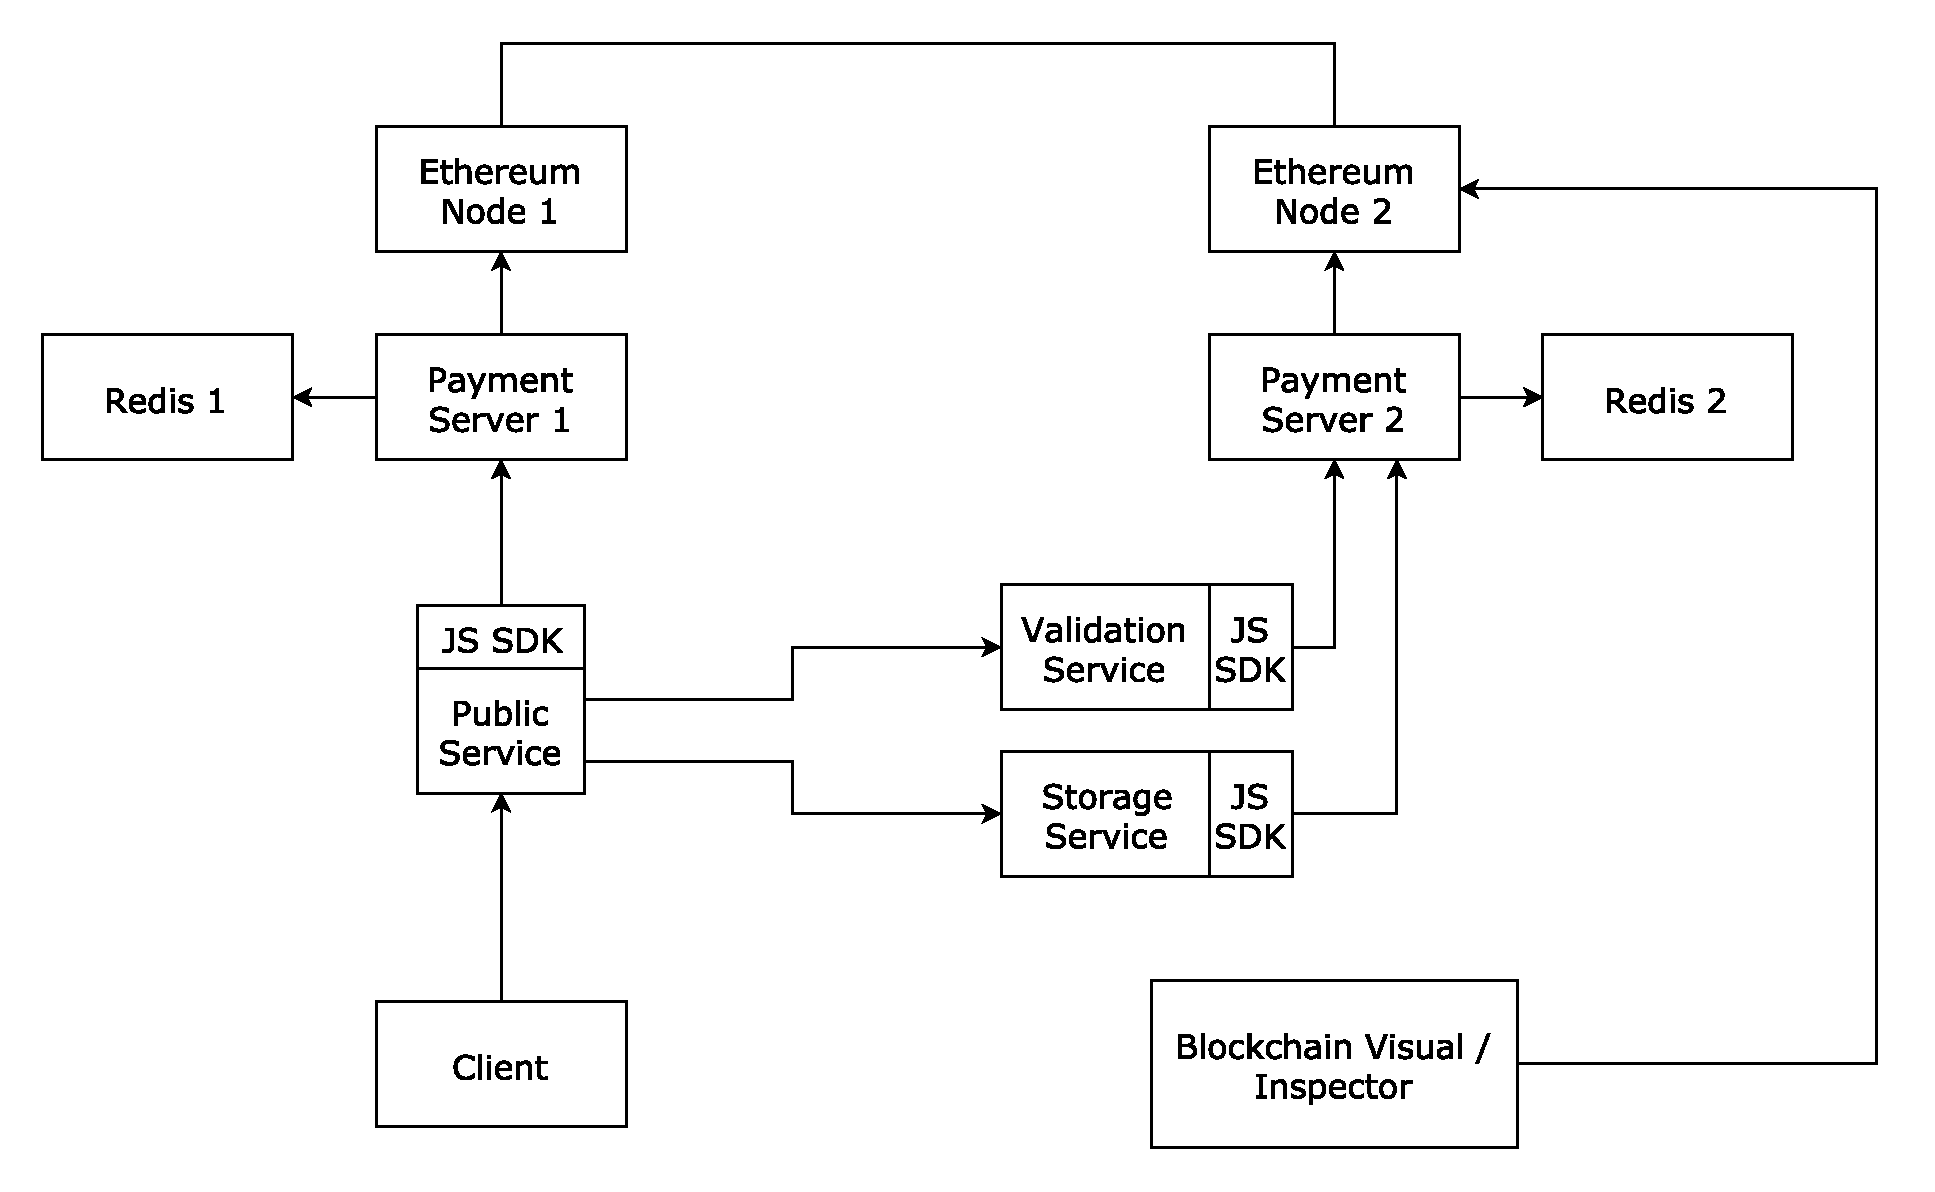
\includegraphics[width=450pt]{Images/PrototypeArchitecture.pdf}
\caption{Prototype architecture.}
\label{fig:PrototypeArchitecture}
\end{figure}

For the test setup Team A runs a publicly available service. This service accepts some user data and first sends it off to a service of Team B to validate the data. If it returns as valid, it sends the data to another service (also hosted by Team B) to store the data. After that, it replies to the initial request with a confirmation.\\
The implementations of the services were stripped down to a minimum because they do not really matter for this test. The important part, which shall be benchmarked, is the communication between the three services.\\

The public service does not require payment by an end user. It can be used via a simple HTTP endpoint. The other two services however must be paid by the public service through the blockchain payment infrastructure.\\
Figure \ref{fig:ServiceInteractionFlow} shows the interaction flow between the services, their Payment Servers and the end consumer client.\\

\begin{figure}[H]
\centering
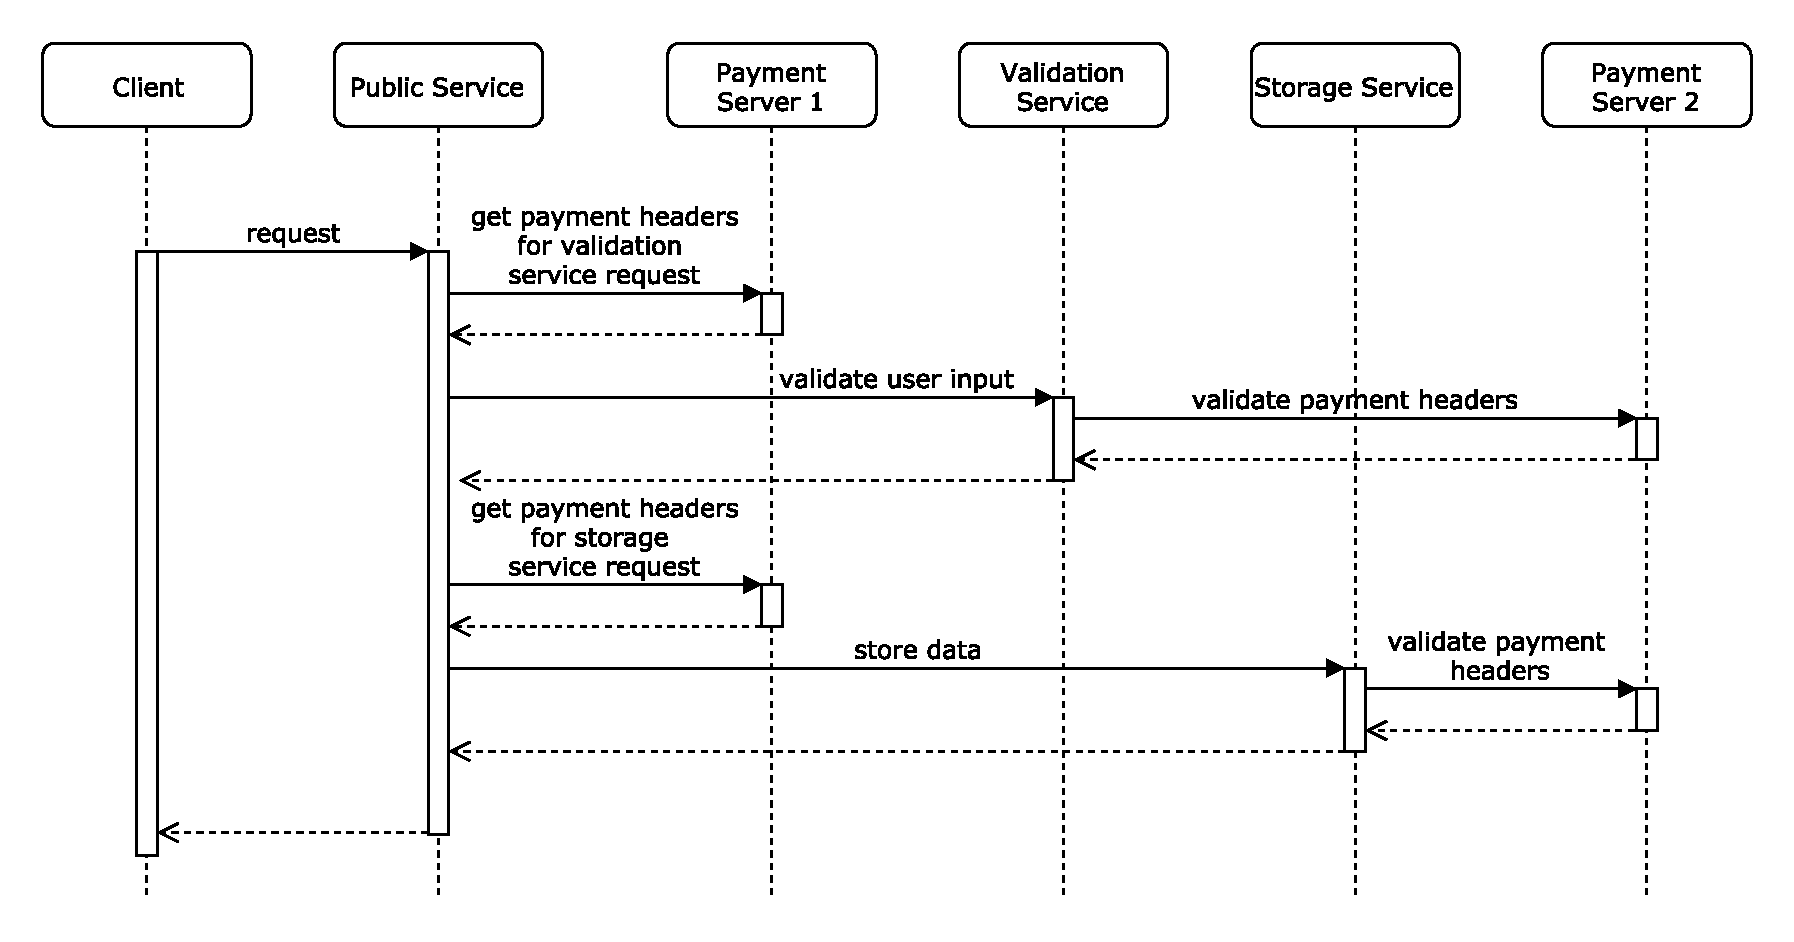
\includegraphics[width=450pt]{Images/ServiceInteractionFlow.pdf}
\caption{Service interaction flow.}
\label{fig:ServiceInteractionFlow}
\end{figure}

Additionally, the blockchain inspection interface can be connected to an Ethereum node of either team - or also to a dedicated Ethereum node. Through this, transactions and blocks on the chain can be inspected.

\subsection{Token Redemption Code Samples}

The heart of the system is the so called Intermediary smart contract which gets deployed on the blockchain for each service relationship. The Ethereum ecosystem offers several programming languages to write such contracts. For this prototype Solidity \cite{web52} was chosen. It is similar to JavaScript but contains static typing.\\
A contract itself can be compared to a class in object-oriented programming languages. It defines local variables to store data and functions that can be called from the outside. A deployed contract can be seen as an instance of a class.\\

It is worth noting that read-only operations, like getting the state of an instance variable can be done for free through a so-called "call". Any state change however, needs to be performed as a blockchain transaction and therefore costs gas and takes time to be mined into the blockchain.\\

To give an example of how the contract works, the implemented token redemption flow shall be presented in more detail.\\

As stated in the "System Design Token Redemption" chapter, the token redemption flow consists of two stages. First the service provider performs a transaction to announce that it wants to redeem a token. After the timeout passed, it initiates a second transaction to complete the redemption.\\

Listing \ref{lst:tokenredemption1} shows the function to start the token redemption.\\

\begin{lstlisting}[caption={Start token redemption.},label=lst:tokenredemption1]
function startTokenRedemption(uint newTokenId) public {
  if (terminated) { Error(1); return; } // I
  if (msg.sender != serviceProvider) { Error(2); return; } // II
  if (newTokenId == activeTokenId) { Error(31); return; }  // III
  if (redeemedTokenIds[newTokenId] > 0) { Error(33); return; }  // IV
  if (soonExpiringTokenId != 0) { Error(32); return; }  // V

  soonExpiringTokenId = activeTokenId; // VI
  soonExpiringTokenIdTimeout = now + tokenRedemptionTimeout; // VII
  if (terminationStartedAt == 0) {
    activeTokenId = newTokenId;
  } else {
    activeTokenId = 0;
  }
}
\end{lstlisting}

At first, this method performs a couple of safety checks and aborts further execution if they fail.\\
It is worth noting that it also records an "Error" event to communicate the reason for the failure. Because of the way that transactions work in Ethereum it is not possible for them to provide a return value like in usual programming languages. Instead events can be fired by the contract that get recorded and can be analyzed later on.\\
The error is communicated via a numeric code to save the somewhat expensive storage space on the chain. A mapping of error codes to human readable representations is done in the Payment Server.\\

The performed checks ensure that:
\begin{itemize}
\item[] I) The contract is still active and was not terminated yet.
\item[] II) The sender is the service provider. This is checked by Ethereum leveraging the public key infrastructure. To trigger this action one needs to have access to the private key of the service provider.
\item[] III \& IV) The newly provided token ID was not used ever before.
\item[] V) No other token redemption is currently active for this contract.
\end{itemize}

The new token ID must be passed in to this function because it needs to be a unique value, e.g. generated based on a Universal Unique Identifier (UUID ) \cite{web53}, but the code must also be deterministic. The contract cannot generate random numbers for a UUID itself because it then would create different results when running on different machines in the Ethereum network.\\

After these initial checks the current token ID is stored as "soon expiring" (VI) and the point in time, from which on the token redemption can be completed, is calculated and stored as well (VII).\\

If the termination of the contract was not yet started, the provided token ID is stored as the new active ID now. If the termination was already started, the active token ID is set to zero to indicate that the last token for this contract was now redeemed and that no further requests can be paid with it.\\
This avoids the case of creating a new token during the termination timeout period, which possibly cannot be redeemed anymore until the termination timeout passes.\\

Listing \ref{lst:tokenredemption2} shows the function to finalize the token redemption. It will be invoked by the Payment Server after the timeout passed.\\

\begin{lstlisting}[caption={Finalize token redemption.},label=lst:tokenredemption2]
function redeemToken(uint numRequests, bytes32 hash, uint8 v, bytes32 r, bytes32 s) public {
  if (terminated) { Error(1); return; } // I
  if (msg.sender != serviceProvider) { Error(2); return; }  // II
  if (now < soonExpiringTokenIdTimeout) { Error(30); return; }  // III
  if (soonExpiringTokenId == 0) { Error(39); return; } // IV

  if (sha256(serviceConsumer, soonExpiringTokenId, this, numRequests) != hash) { Error(4); return; } // V
  if(ecrecover(hash, v, r, s) != serviceConsumer) { Error(4); return; } // VI

  uint amount = costPerRequest * numRequests; // VII
  if (amount > serviceConsumerFunds) { Error(34); return; } // VIII

  redeemedTokenIds[soonExpiringTokenId] = amount; // IX
  soonExpiringTokenId = 0;  // X
  soonExpiringTokenIdTimeout = 0; // XI
  serviceConsumerFunds = serviceConsumerFunds - amount; // XII
  serviceProviderFunds = serviceProviderFunds + amount; // XIII

  Redeemed(amount); // XIV
}
\end{lstlisting}

This function takes several parameters. First of all, it requires the final number of requests that are covered by the token. The remaining parameters (hash, v, r, s) specify the signature with which the token is signed. The signature therefore is based on the sha256 hash of the address of the service consumer $C$, the ID of the token $T_{ID}$, the address of the intermediary contract $I$ and the number of requests $R$.\\
The function first performs some validity checks. Again the contract must not be terminated (I) and the function can only be invoked by the service provider (II). The function also aborts when the timeout did not pass yet (III) or no token redemption was started at all (IV).\\

After these trivial checks, it first checks the supplied hash (V) and then uses the built in "ecrecover" function to validate the signature. Ecrecover computes the address of the signer based on the payload data hash and the signature parameters. If that address does not match the expected consumers address, the signature and therefore the token is not valid.\\

When all these checks passed, the value of the token is calculated (VII). If this exceeds the consumer's funds, the transaction is canceled as well (VIII). One could argue to then at least transfer all what is left of the consumer's funds. However, the service provider is the only one to redeem tokens. Therefore, it is the only one to reduce the funds of the consumer locked inside the contract. So it is its responsibility to check if enough funds exist for a token, as soon as the request with that token arrives.\\

The transferred amount is stored in a map (IX). This marks the token as used and can also be used as a history of redeemed tokens for further analysis.\\
The soon expiring token parameters are resetted (X \& XI) and the funds are transferred between the parties inside the contract (XII \& XIII).\\

In the end a "Redeemed" event is fired (XIV). It can be used to validate the successful execution of this function and for further analysis later on.

\subsection{Advanced Caching}

Whenever a request is signed or verified by the Payment Server, several checks need to be performed based on the current state in the contract. Specifically the active token ID must be known during signature creation and verification. During verification the consumers funds also need to be checked, as well as if the contract is terminated, and if the contract is setup as expected.\\

All these checks require data from the blockchain and therefore cause calls to the blockchain node. With a lot of requests coming in, this can cause a lot of load on the blockchain node and slows down the process significantly.\\

Fortunately, this data can be cached in the Payment Server.\\
The contract setup (information like cost per request, timeout durations and participants) cannot be changed after the contract was deployed to the blockchain. This makes this data cachable for a possibly unlimited amount of time, e.g. until a restart of the Payment Server.\\
For the token ID, funds and termination status the situation is a bit trickier since their values change over the lifetime of the contract. However, a change to these values is performed with transition periods. This means the token ID and funds can be cached for a fraction of the token redemption timeout and the termination status can be cached for a fraction of the termination timeout.\\

This behavior is implemented in the TimeLimitedCache in the prototype. It also implements an optimistic cache refresh.\\
The cache knows until when a value is valid. If the value is requested the first time it is not in the cache and will be fetched. Further requests for this value will then return the cached value as long as it is valid. If it is requested shortly before it will turn invalid, the cache itself will start an update call to refresh the cache in the background. It still returns the old cached value until it either expires or the new value arrives.\\
This avoids the case, that when the cached value expires the next request would run into a cache miss and would need to wait significantly longer until it gets the value.\\

This time-based caching is what shall be called "Advanced Caching" in this context. It can be seen as further blockchain scaling method for high frequency applications. Even "fast" read-only calls can become a bottleneck, but as long as state changes on the contract happen in two transactions with a transition period in between, values can be cached and increase performance.

\subsection{Timeout Handling}

Token redemption and termination operations are two steps processes with a transition period. This means after triggering the first transaction the second transaction needs to be triggered later on to finalize the redemption or termination.\\

In this prototype, the Payment Servers run periodic checks for pending token redemptions and terminations of the services that they know about. This has the advantage, that the individual microservices do not need to care about this and can be stateless. The downside of this setup is that this puts additional load on the Payment Server.\\

The described way shows only one possibility to address this challenge. Alternatively, the microservices could be responsible to trigger the finalizing transactions or one could build a dedicated service for it. If the contracts run on the public Ethereum network one could also make use of the Ethereum Alarm Clock service \cite{web56} or deploy a similar service on the own private network.\\

The timer infrastructure is also used to redeem open tokens about once per hour. This leads to transparency on the blockchain and is an additional safeguard against failures.

\subsection{Blockchain Inspector Interface}

The blockchain inspector is a web based standalone tool written with React \cite{web36}. It can connect to any Ethereum node via the JSON RPC interface \cite{web23} and inspect the data on the blockchain. The tool can either be deployed on a webserver or can be run locally in the browser.\\
The following figures \ref{fig:BlockchainInspector1}, \ref{fig:BlockchainInspector2} and \ref{fig:BlockchainInspector3} show screenshots of the interface.\\

\begin{figure}[H]
\centering
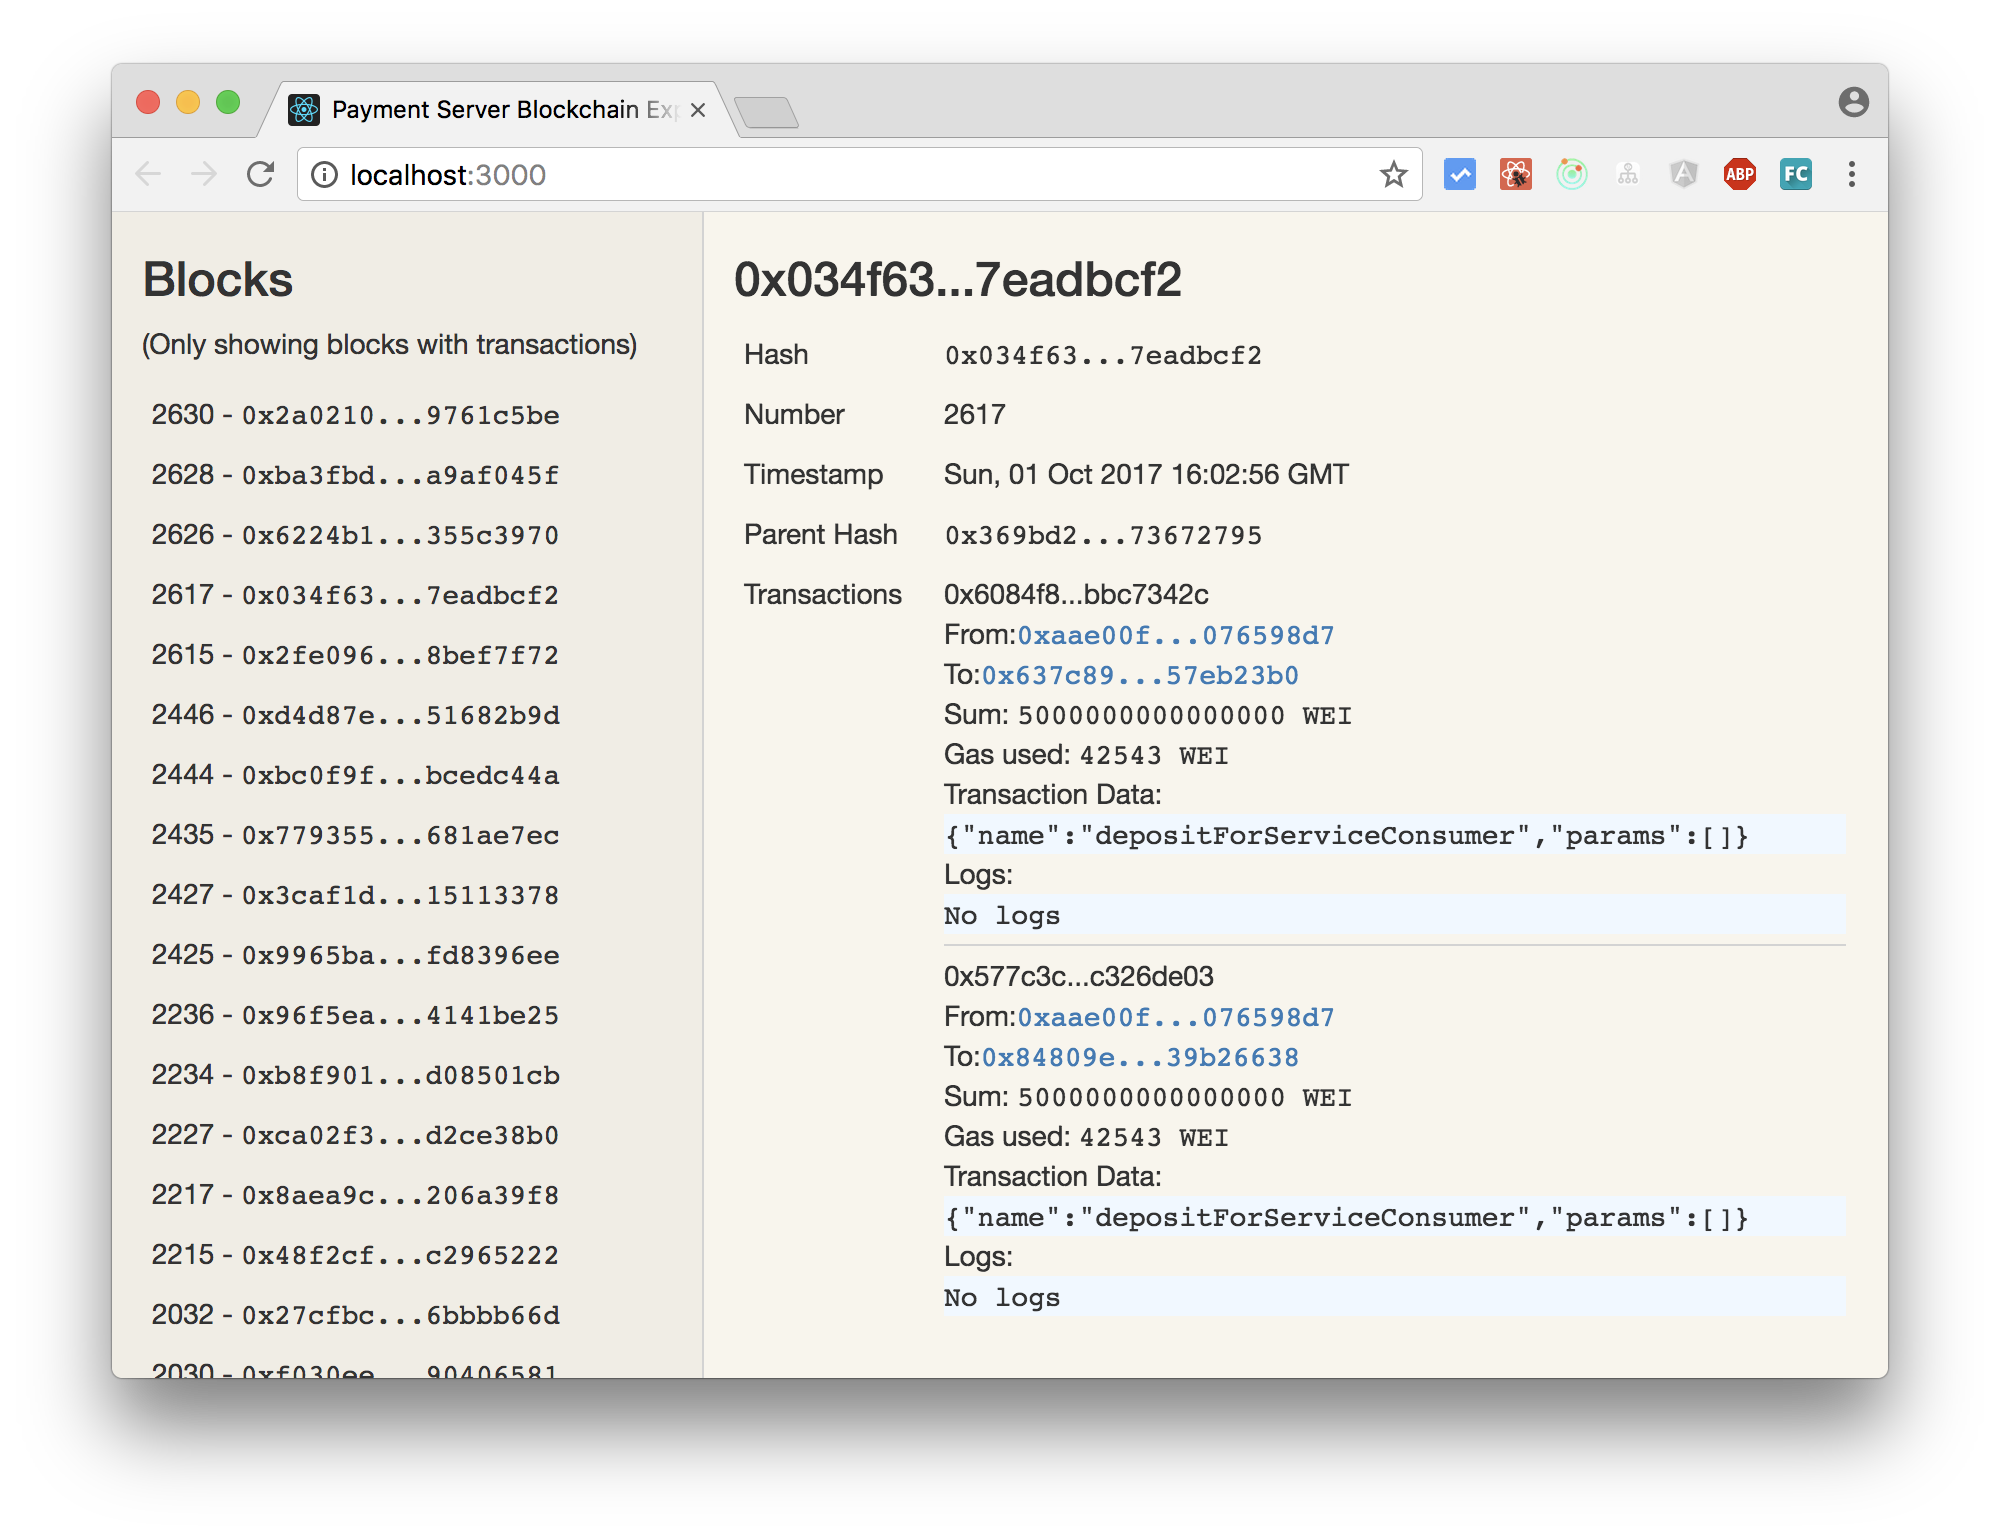
\includegraphics[width=450pt]{Images/Visualizer-Deposit.png}
\caption{Blockchain Inspector - Showing the depositing transaction which funds the payment channel between two parties.}
\label{fig:BlockchainInspector1}
\end{figure}

On the left a list of all blocks in the blockchain that contain relevant transactions is shown. The user can then select a block and see more details about it on the right side. It shows all transactions and also decodes their content and logged events from their binary representations into a readable format.\\

\begin{figure}[H]
\centering
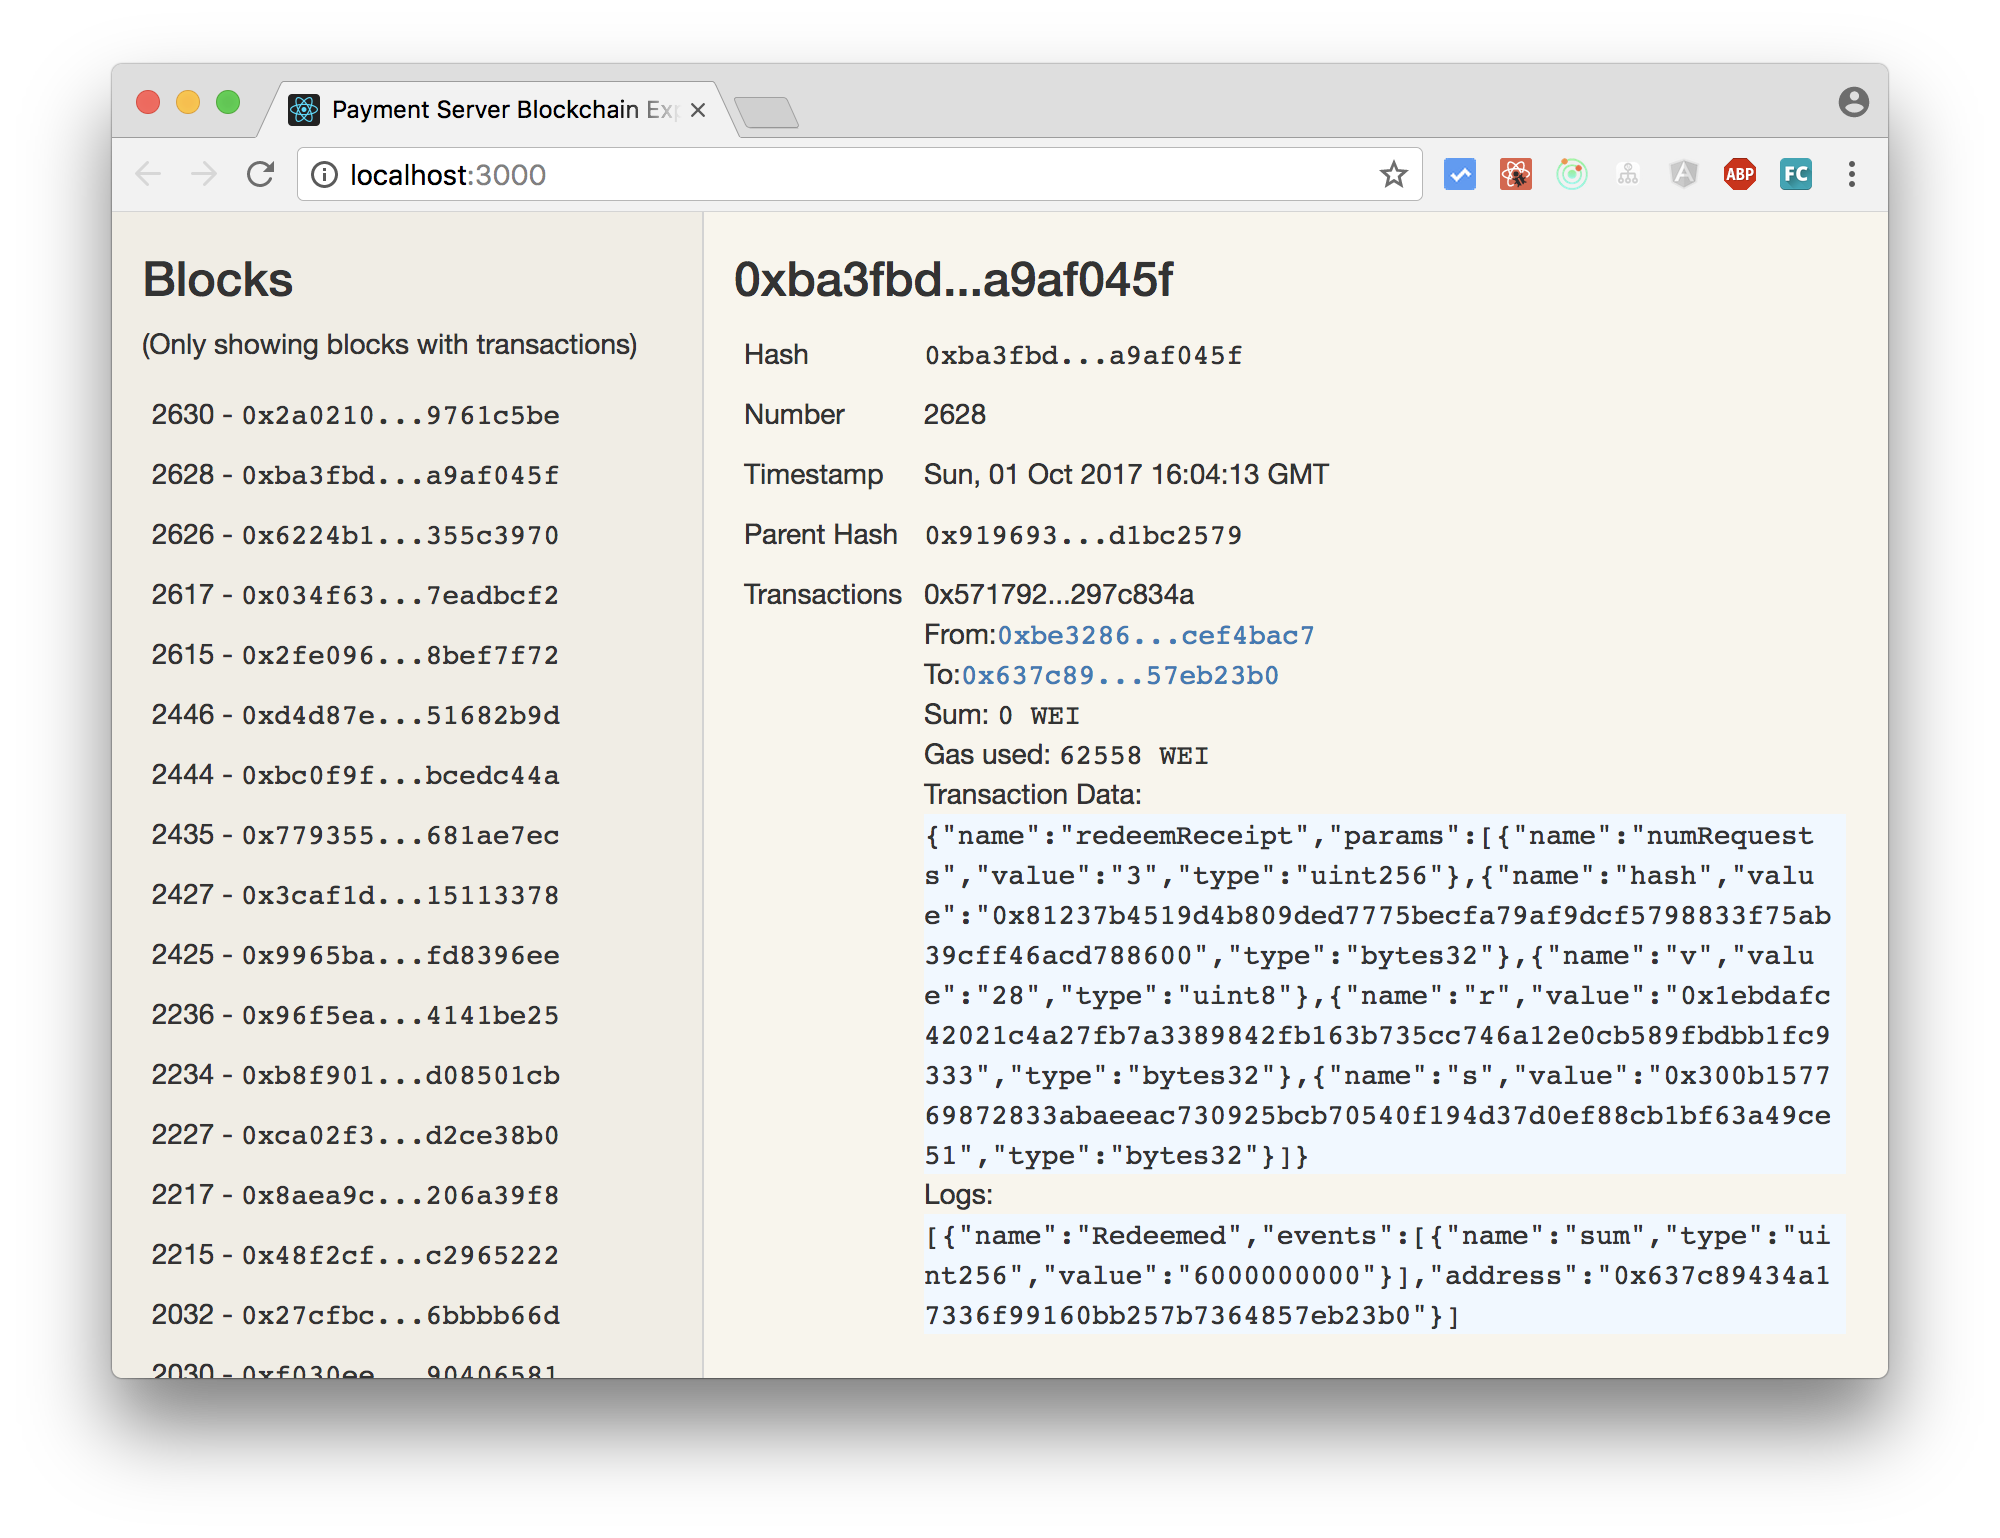
\includegraphics[width=450pt]{Images/Visualizer-FinalizeRedemption.png}
\caption{Blockchain Inspector - Showing a token redemption finalization transaction. Number of requests, token ID and value of the token in ether is stored.}
\label{fig:BlockchainInspector2}
\end{figure}

\begin{figure}[H]
\centering
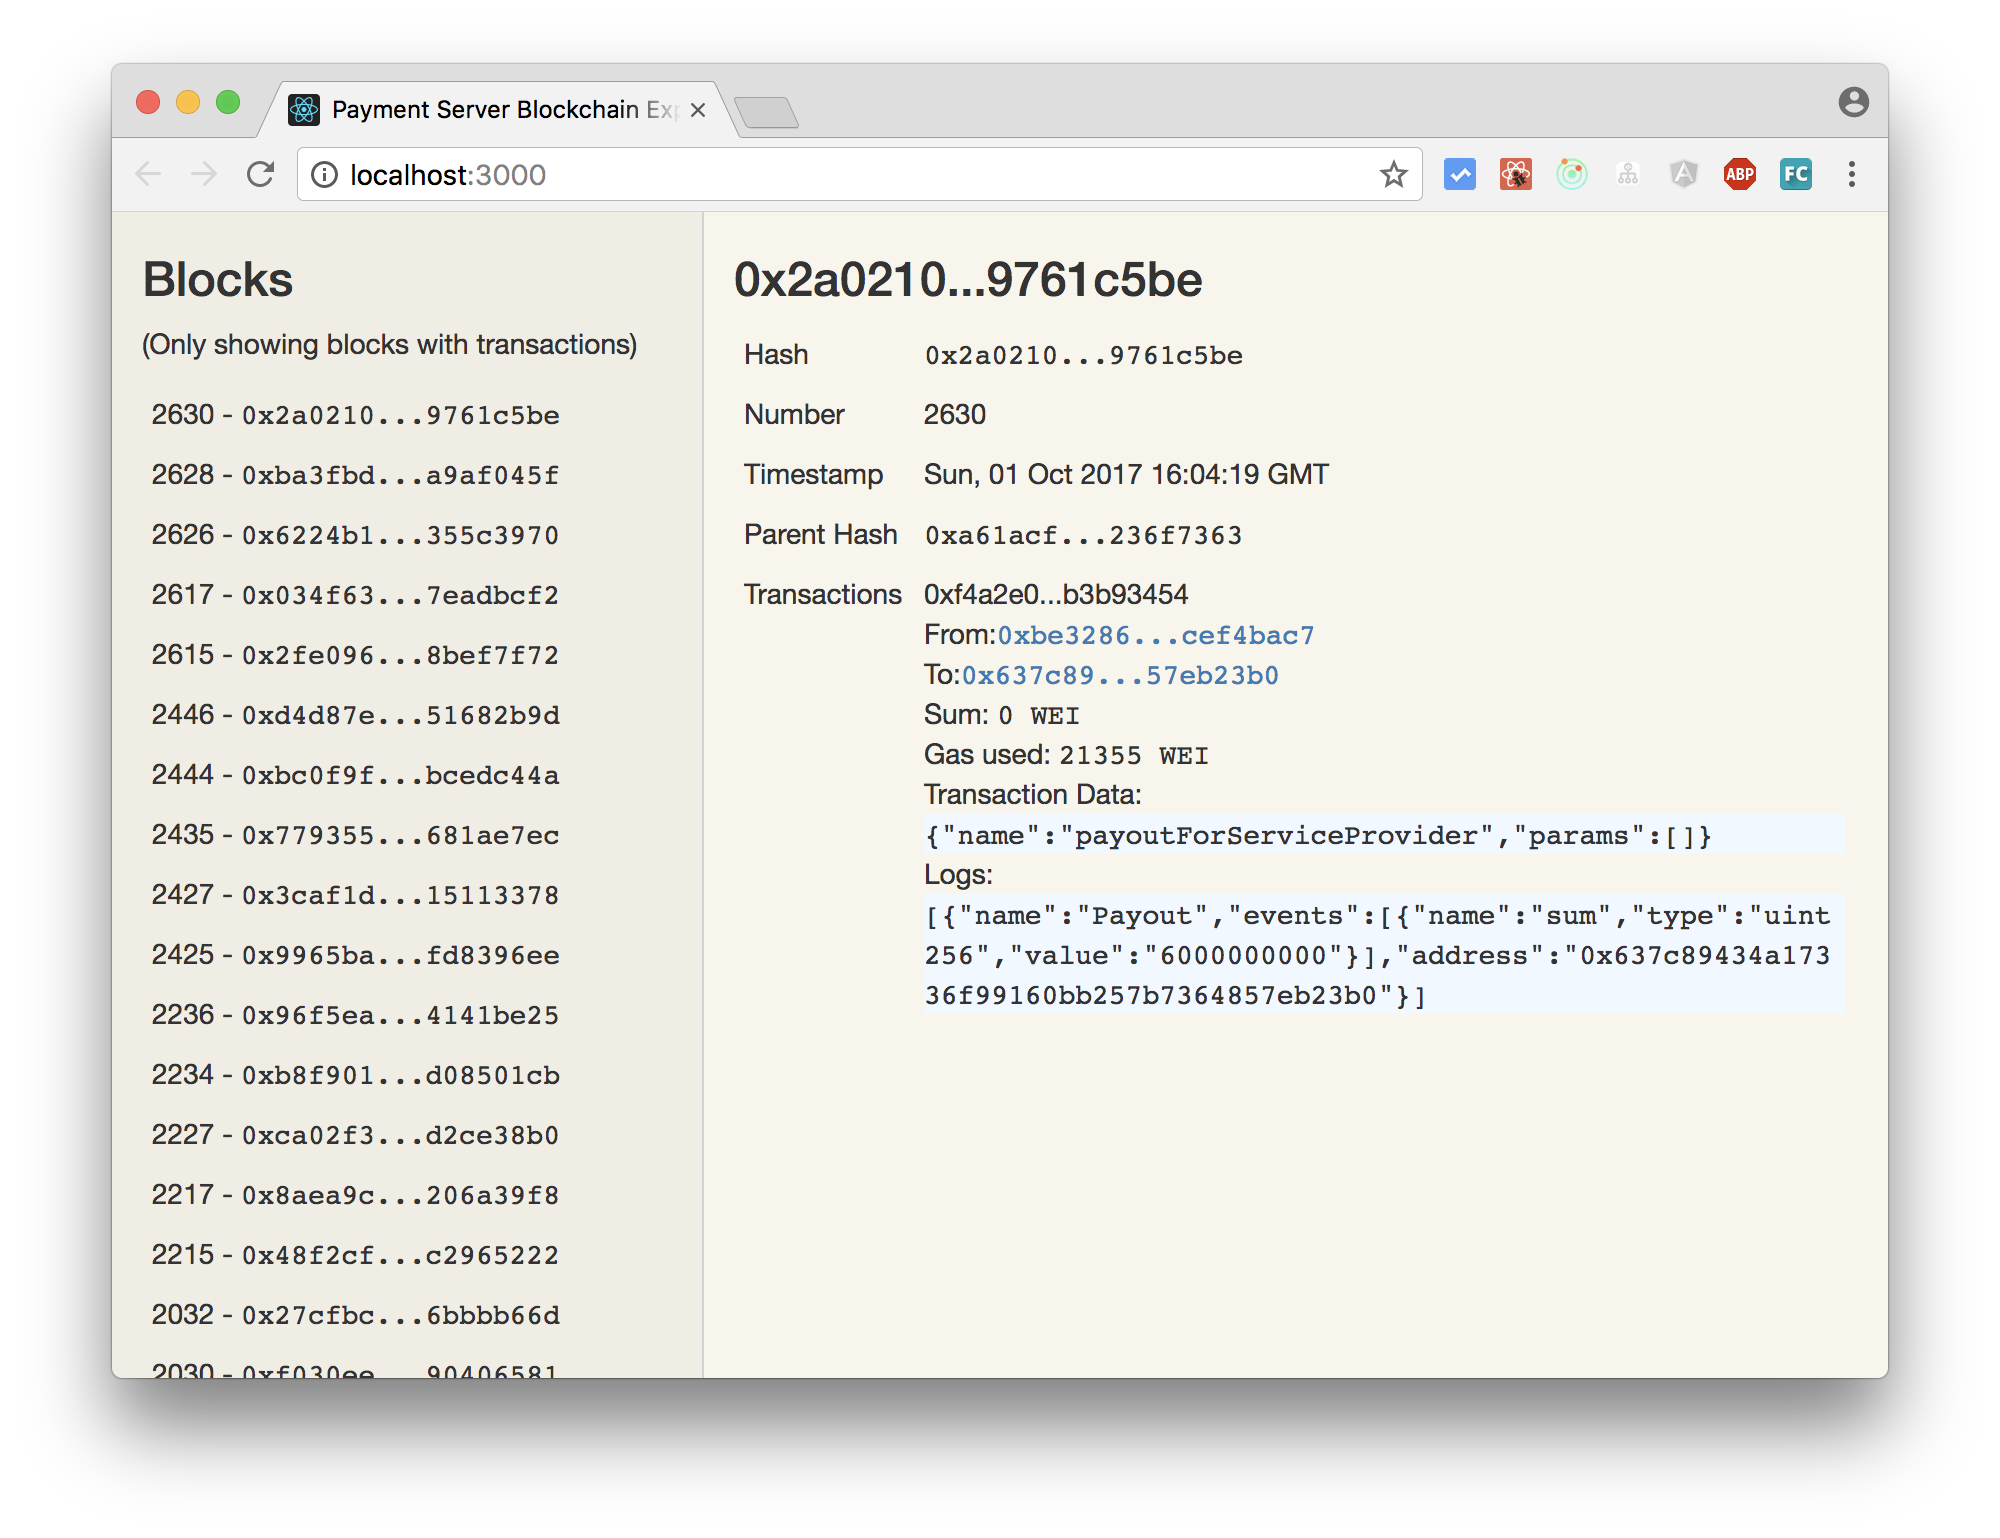
\includegraphics[width=450pt]{Images/Visualizer-Payout.png}
\caption{Blockchain Inspector - Showing a payout transaction that transfers earned funds from the Intermediary to the service provider.}
\label{fig:BlockchainInspector3}
\end{figure}

With this interface, it is easy to follow the performed transactions for contract deployments, token redemptions, payouts and so on. Also the state and flow of funds can be reconstructed through this.


\newpage
\section{Performance Evaluation}

In the following sub-chapters the setup for the performance tests is presented, as well as the results using the implemented prototype. After the presentation of the overall results, a deep-dive anaylsis explains the observed performance characteristics and gives an outlook on how further improvements can be achieved.\\

It should be mentioned that over the course of the implementation of the prototype, several performance tests were executed and emerging bottlenecks were fixed. A great example for this is the advanced caching mentioned above that was added after the blockchain node was discovered as a bottleneck.\\
However, the results and setup presented in this paper are only based on the final setup and implementation.\\

\subsection{Setup}

For the performance tests a setup of four AWS EC2 (Elastic Compute Cloud) \cite{awsec2} instances was used in the eu-west-1 region. For the specification of the EC2 instance types (m3.large, t2.large, ...) and region specifications (e.g. eu-west-1) please refer to Amazon's official documentation about AWS \cite{web38}.
\begin{itemize}
\item Two m3.large instance each running one Geth Ethereum node in a Docker container.
\item One t2.large instance running the Payment Servers, Redis servers and microservices in Docker containers orchestrated via Docker compose.
\item One t2.medium instance used to generate load against the system.
\end{itemize}

The services and communication patterns follow the outlined architecture from the previous chapter. The load generating instance called the public endpoint of the public service over http. For the communication between the services their public IPs were used. Every service and Payment Server was deployed exactly once, so no load balancers were used in this setup.\\

To generate load the Apache Bench \cite{web54} tool was used and ran in four different configurations.
\begin{itemize}
\item 100 requests with a concurrency of just one request.
\item 500 requests with a concurrency of five requests at a time.
\item 1000 requests with a concurrency of ten requests at a time.
\item 2000 requests with a concurrency of 20 requests at a time.
\end{itemize}

\subsection{Results}

Table \ref{tab:OverallRequestTimesTable} and figure \ref{fig:OverallRequestTimesDiagram} show an overview of the request times measured by Apache Bench. Note that this includes the full interaction between all services. Overall, one request to the public service triggers two calls to the Payment Server to create signatures, one call to the validation and one call to the persistence service. Each of them performs one signature verification call to the Payment Server.\\

\begin{table}[H]
    \centering
    \label{tab:OverallRequestTimesTable}
    \begin{tabular}{|l|c|c|c|c|}
        \hline
        &   c=1 n=100   & c=5 n=500 &   c=10 n=1000 & c=20 n=2000\\
        \hline
        50 \%   &   43          &   123     &   223         &   442\\
        \hline
        80 \%   &   46          &   142     &   269         &   500\\
        \hline
        90 \%   &   52          &   156     &   307         &   539\\
        \hline
        95 \%   &   61          &   173     &   346         &   586\\
        \hline
        98 \%   &   75          &   200     &   384         &   634\\
        \hline
        99 \%   &   82          &   236     &   508         &   665\\
        \hline
        100 \%   &   82          &   317     &   757         &   836\\
        \hline
        \hline
        Requests/Second   &   22,48          &   39,35     &   41,96         &   44,59\\
        \hline
    \end{tabular}
    \caption{Overall request times in milliseconds (ms).}
\end{table}

\begin{figure}[H]
\centering
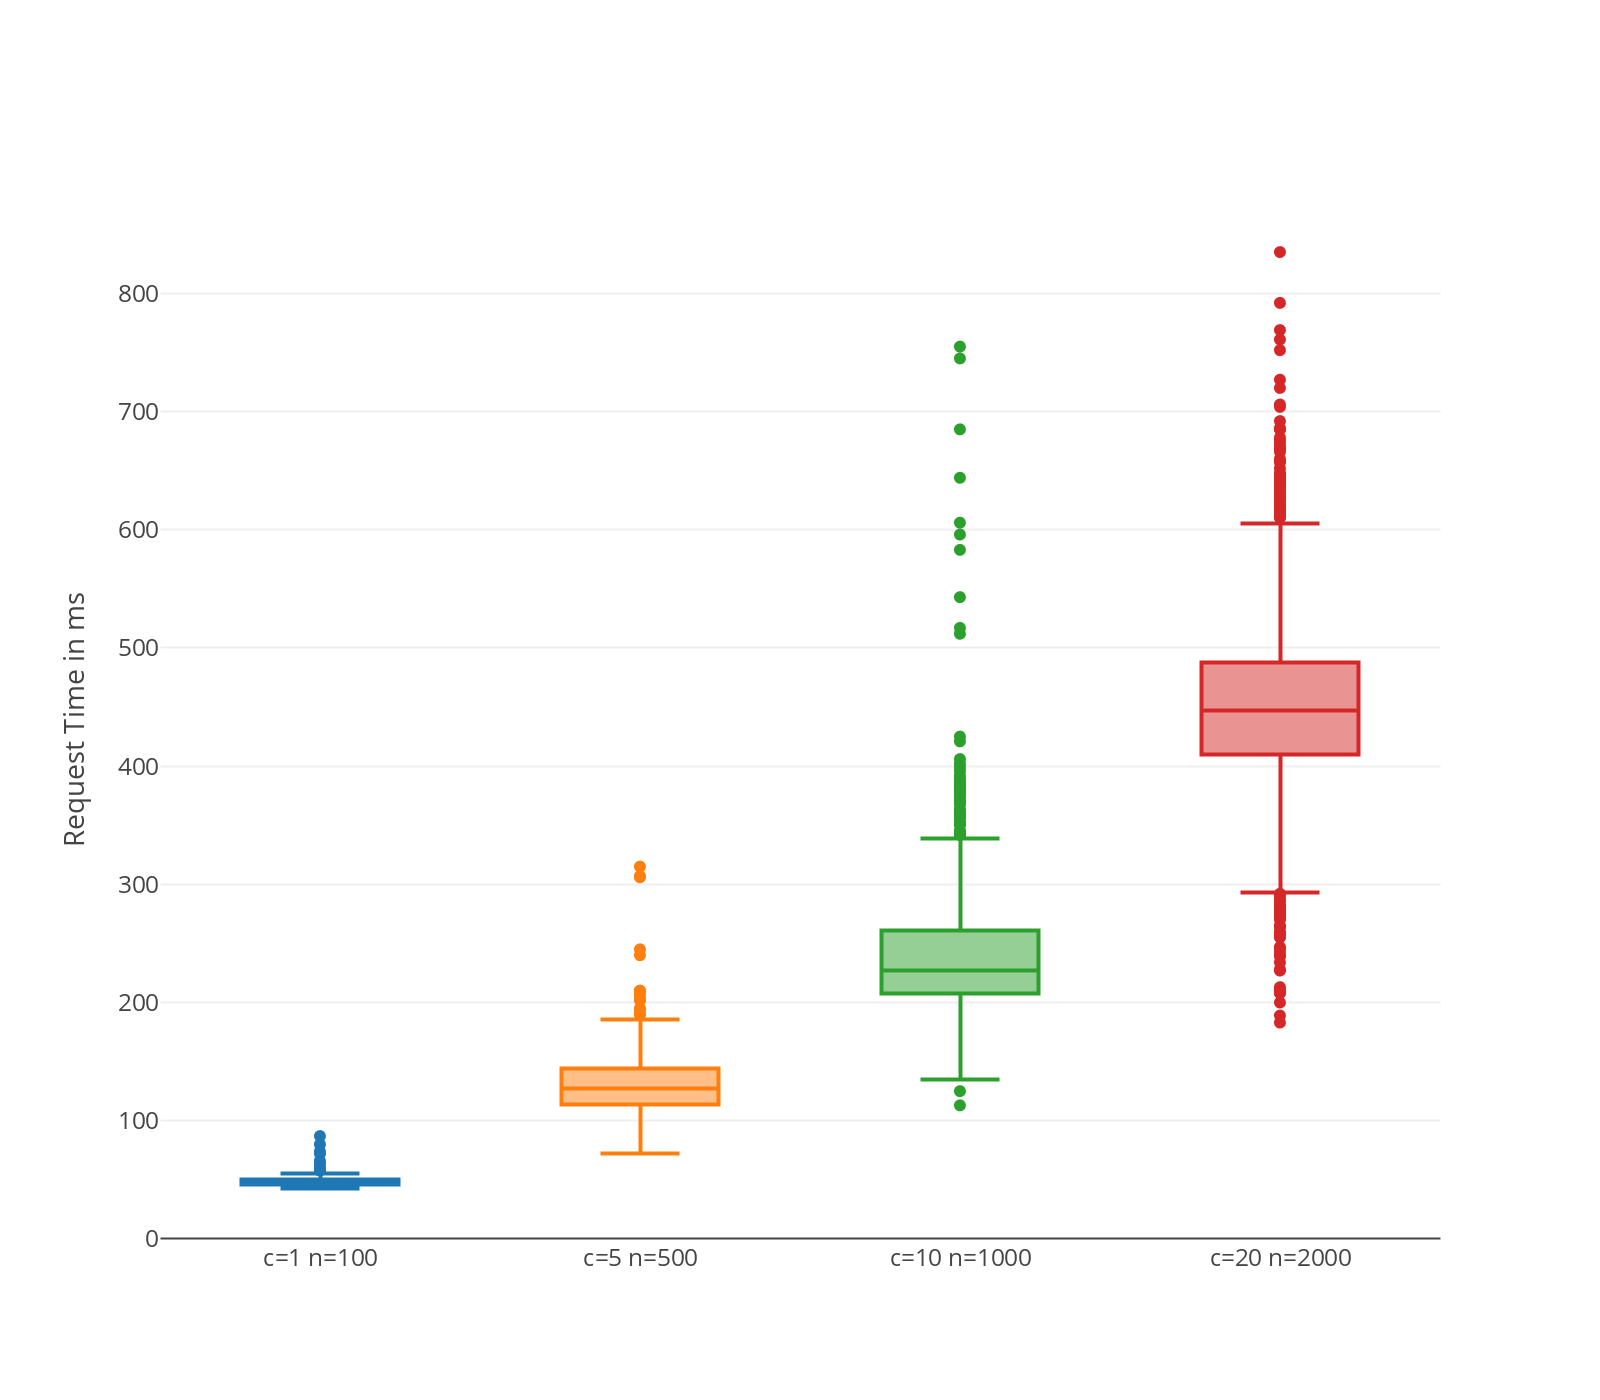
\includegraphics[width=350pt]{Images/OverallRequestTimesDiagram.png}
\caption{Graphic representation of overall request times in ms.}
\label{fig:OverallRequestTimesDiagram}
\end{figure}

For a single concurrent request, the response times are in an acceptable range of below 100 ms. As soon as five concurrent requests take place though, the response times increase to about 120-200 ms with outliers to above 300 ms. This is still acceptable for many use-cases and already handles about 40 requests per second or about 140.000 requests per hour, which is already a significant amount for a single instance setup.\\

Scaling to even more concurrent requests leads as expected to worse performance. However, it is worth noting that before the optimized caching was implemented the performance was significantly worse. The request times for concurrent requests reached a threshold of multiple seconds very fast. This was due to the Ethereum node being a significant bottleneck.\\

\subsection{Analysis}

Investigating the response times further, it becomes apparent that the Payment Servers are the bottleneck of the system. Figures \ref{fig:ValidateRequestDurations} and \ref{fig:SignRequestDurations} show the durations that the Payment Server needs to answer signature validation and signature creation requests. They need to sign and verify all requests that happen between the services. The question now is what makes them so slow when multiple requests are coming in at once. After all, it was fast for single requests and nearly all data is cached in memory.\\

\begin{figure}[H]
\centering
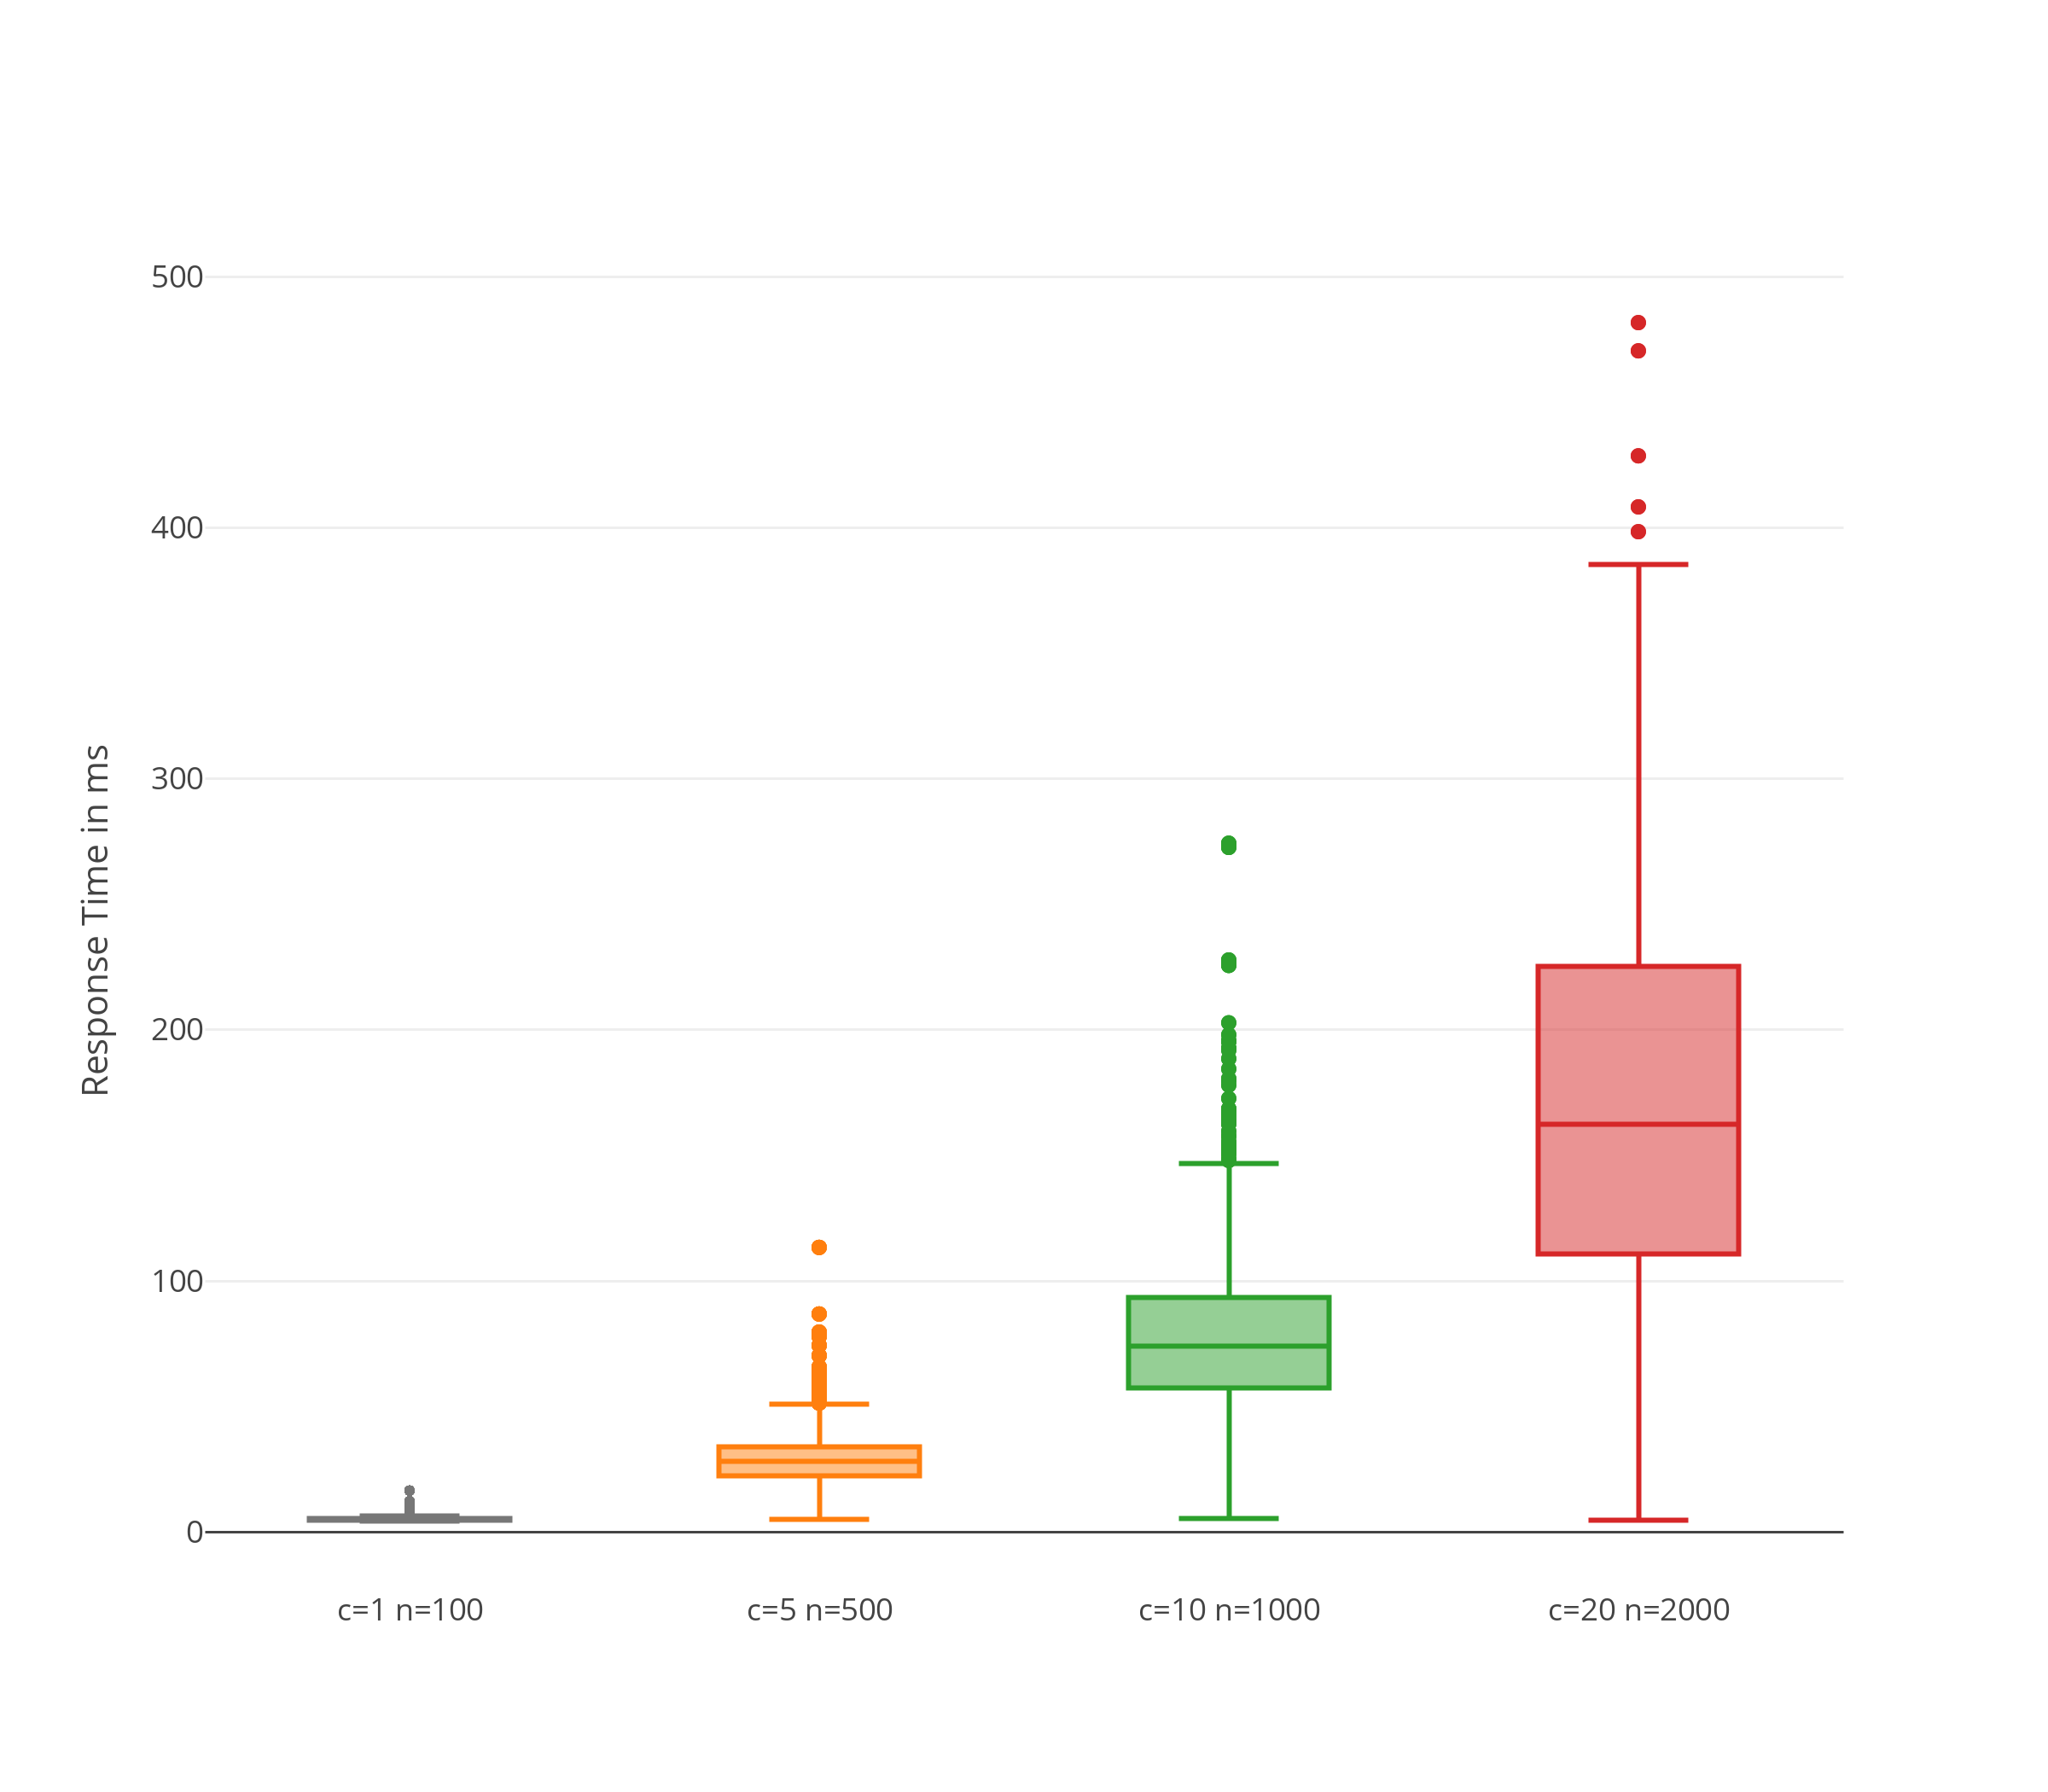
\includegraphics[width=350pt]{Images/ValidateRequestDurations.png}
\caption{Graphic representation of validation request durations in ms.}
\label{fig:ValidateRequestDurations}
\end{figure}

\begin{figure}[H]
\centering
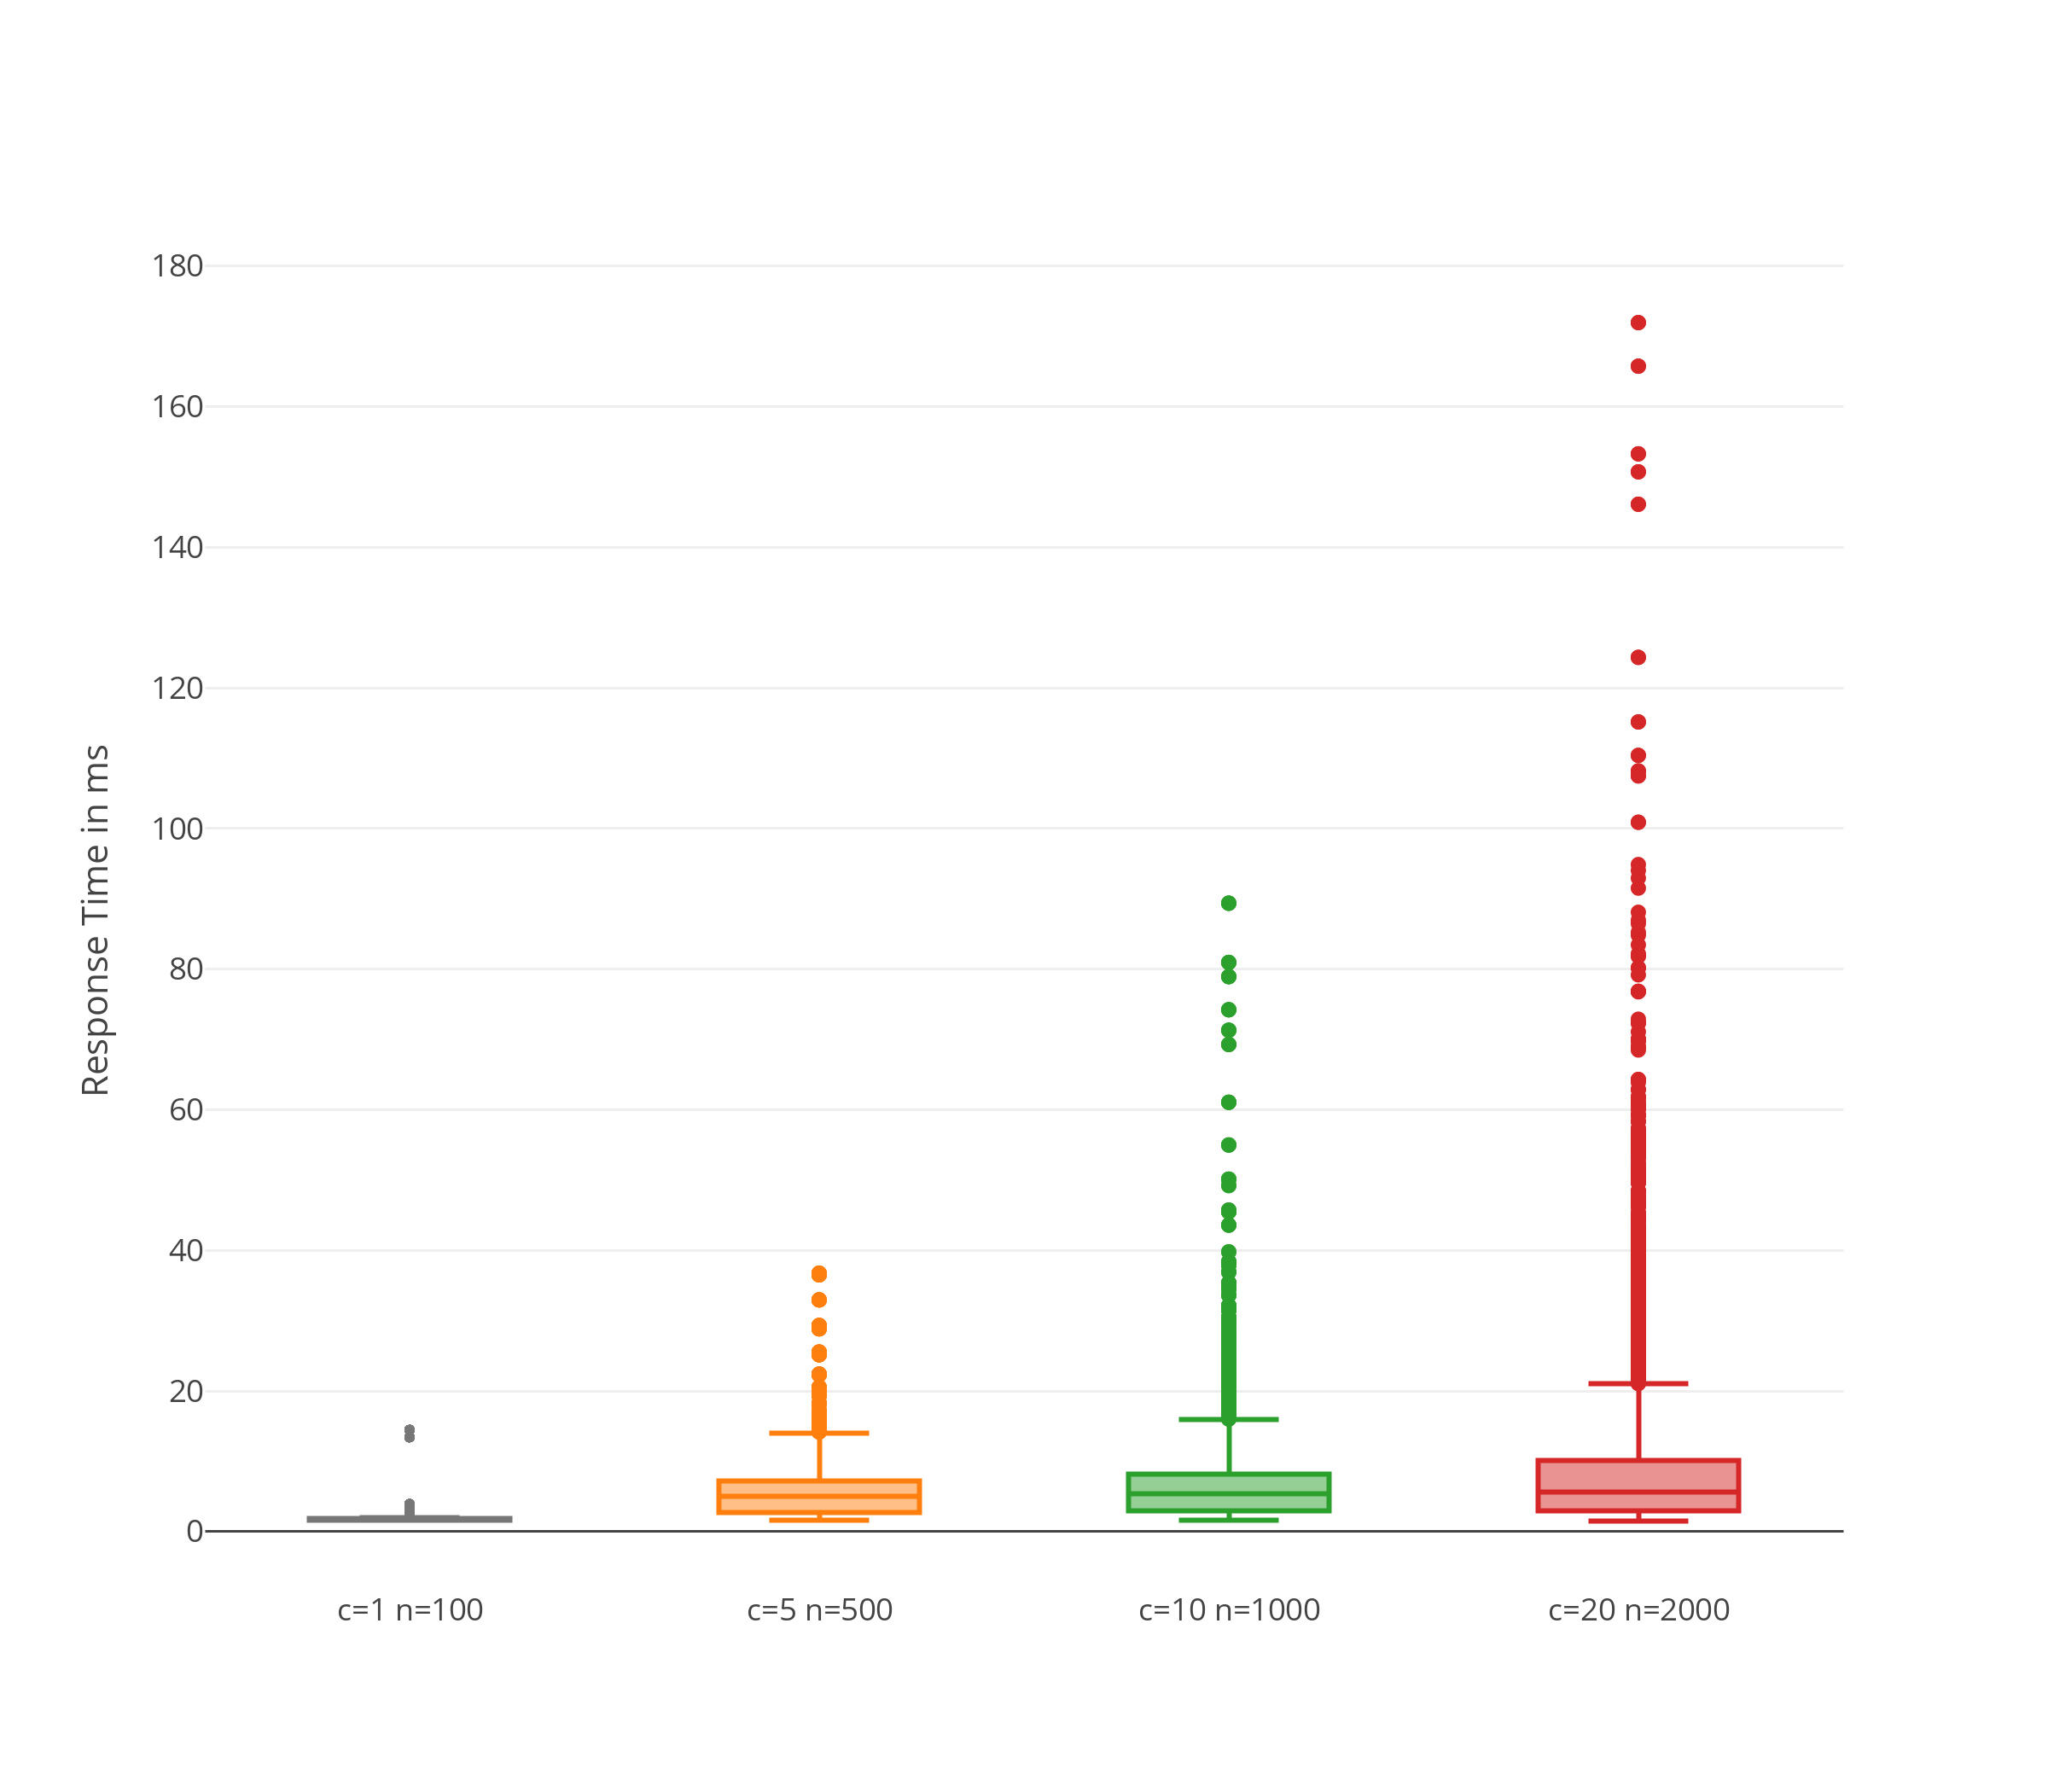
\includegraphics[width=350pt]{Images/SignRequestDurations.png}
\caption{Graphic representation of signing request durations in ms.}
\label{fig:SignRequestDurations}
\end{figure}

To understand this, further knowledge and insights about node.js are required: Node.js is single threaded and based on a so-called event loop \cite{web57}. All incoming events (e.g. an incoming network request or the callback of a file that finished loading from disk) are put in a queue for the event loop. Simplified the event loop executes all these elements in the queue synchronously one after another. All asynchronous calls, e.g. network requests or disk accesses, are put off the queue and not waited for on the queue. This usually makes node.js great for dealing with asynchronous tasks. It can already start processing the next task from the event loop while still waiting for the result of an earlier one. Its result will just be queued into the event loop queue later on.\\
However, this approach is not good for CPU intensive computations because they will block the event loop and prohibit the execution of other events until they are done.

Beside some minor synchronous work for the business logic and json parsing, the Payment Servers are performing cryptographic signature operations to create and verify signatures. These cryptographic operations are CPU intensive. Table \ref{tab:TableSignatureTimes} shows the times to create and verify signatures during the different test runs. The numbers are (except for some outliers) not much different for the different load scenarios. Also the numbers seem not to be really large, as the signature computing time of one to five milliseconds seems fast. However, these numbers add up. If 20 requests hit the server at once, the last request needs to wait at least for 19 to 95 ms just for the other requests to finish their signature validation.\\
Additionally, not only the token signature needs to be checked, but also the signature of the request from the microservice that asked for verification. This adds roughly the same overhead again.\\

\begin{table}[H]
    \centering
    \label{tab:TableSignatureTimes}
    \begin{tabular}{|l|c|c|c|c|c|c|c|c|}
        \hline
        & \multicolumn{4}{|c|}{Validate Signature} & \multicolumn{4}{|c|}{Create Signature}\\
        \hline
        &   c=1   & c=5 &   c=10 & c=20 &   c=1   & c=5 &   c=10 & c=20\\
        \hline
        50 \%   &   3,1     &   3,3 &   3,2 &   3,2 &   1,1 &   1,3 &   1,3 &   1,3\\
        \hline
        80 \%   &   3,7     &   4,0 &   3,9 &   3,8 &   1,2 &   1,7 &   1,9 &   1,8\\
        \hline
        90 \%   &   4,0     &   4,7 &   4,7 &   4,7 &   1,7 &   2,3 &   2,7 &   2,5\\
        \hline
        95 \%   &   4,2     &   5,6 &   5,9 &   5,6 &   1,9 &   2,8 &   3,7 &   3,3\\
        \hline
        98 \%   &   4,9     &   7,1 &   8,6 &   7,3 &   1,9 &   3,8 &   5,4 &   4,3\\
        \hline
        99 \%   &   5,2     &   8,5 &   10,3 &   9,1 &  2,0 &   4,3 &   7,2 &   5,4\\
        \hline
        100 \%  &   8,4     &   12,2 &   29,6 &   34,6 & 2,1 &  11,1 &  19,6 &  19,4\\
        \hline
    \end{tabular}
    \caption{Signature computing time in ms.}
\end{table}

This causes requests to get stuck for some time until they get started to be processed. This effect can be seen in table \ref{tab:TableWaitDurations} and figures \ref{fig:ValidateRequestWaitDurationsDiagram} \& \ref{fig:CreateSignatureWaitDurationsDiagram} which show the time a request took from being sent by the microservice until the Payment Server first starts processing it.\\

\begin{table}[H]
    \centering
    \label{tab:TableWaitDurations}
    \begin{tabular}{|l|c|c|c|c|c|c|c|c|}
        \hline
        & \multicolumn{4}{|c|}{Validate Signature} & \multicolumn{4}{|c|}{Create Signature}\\
        \hline
        &   c=1   & c=5 &   c=10 & c=20 &   c=1   & c=5 &   c=10 & c=20\\
        \hline
        50 \%   &   5     &   11 &   13 &   14 &   5 &   8 &   8 &   8\\
        \hline
        80 \%   &   6     &   17 &   21 &   25 &   5 &   13 &   15 &   18\\
        \hline
        90 \%   &   6     &   21 &   27 &   43 &   6 &   17 &   23 &   41\\
        \hline
        95 \%   &   7     &   24 &   34 &   68 &   6 &   20 &   34 &   62\\
        \hline
        98 \%   &   9     &   29 &   44 &   87 &   6 &   25 &   50 &   78\\
        \hline
        99 \%   &   9     &   31 &   59 &   98 &  7 &   27 &   58 &   89\\
        \hline
        100 \%  &   22     &   48 &   184 &   143 & 19 &  33 &  92 &  119\\
        \hline
    \end{tabular}
    \caption{Wait durations until first processing of requests in ms.}
\end{table}

\begin{figure}[H]
\centering
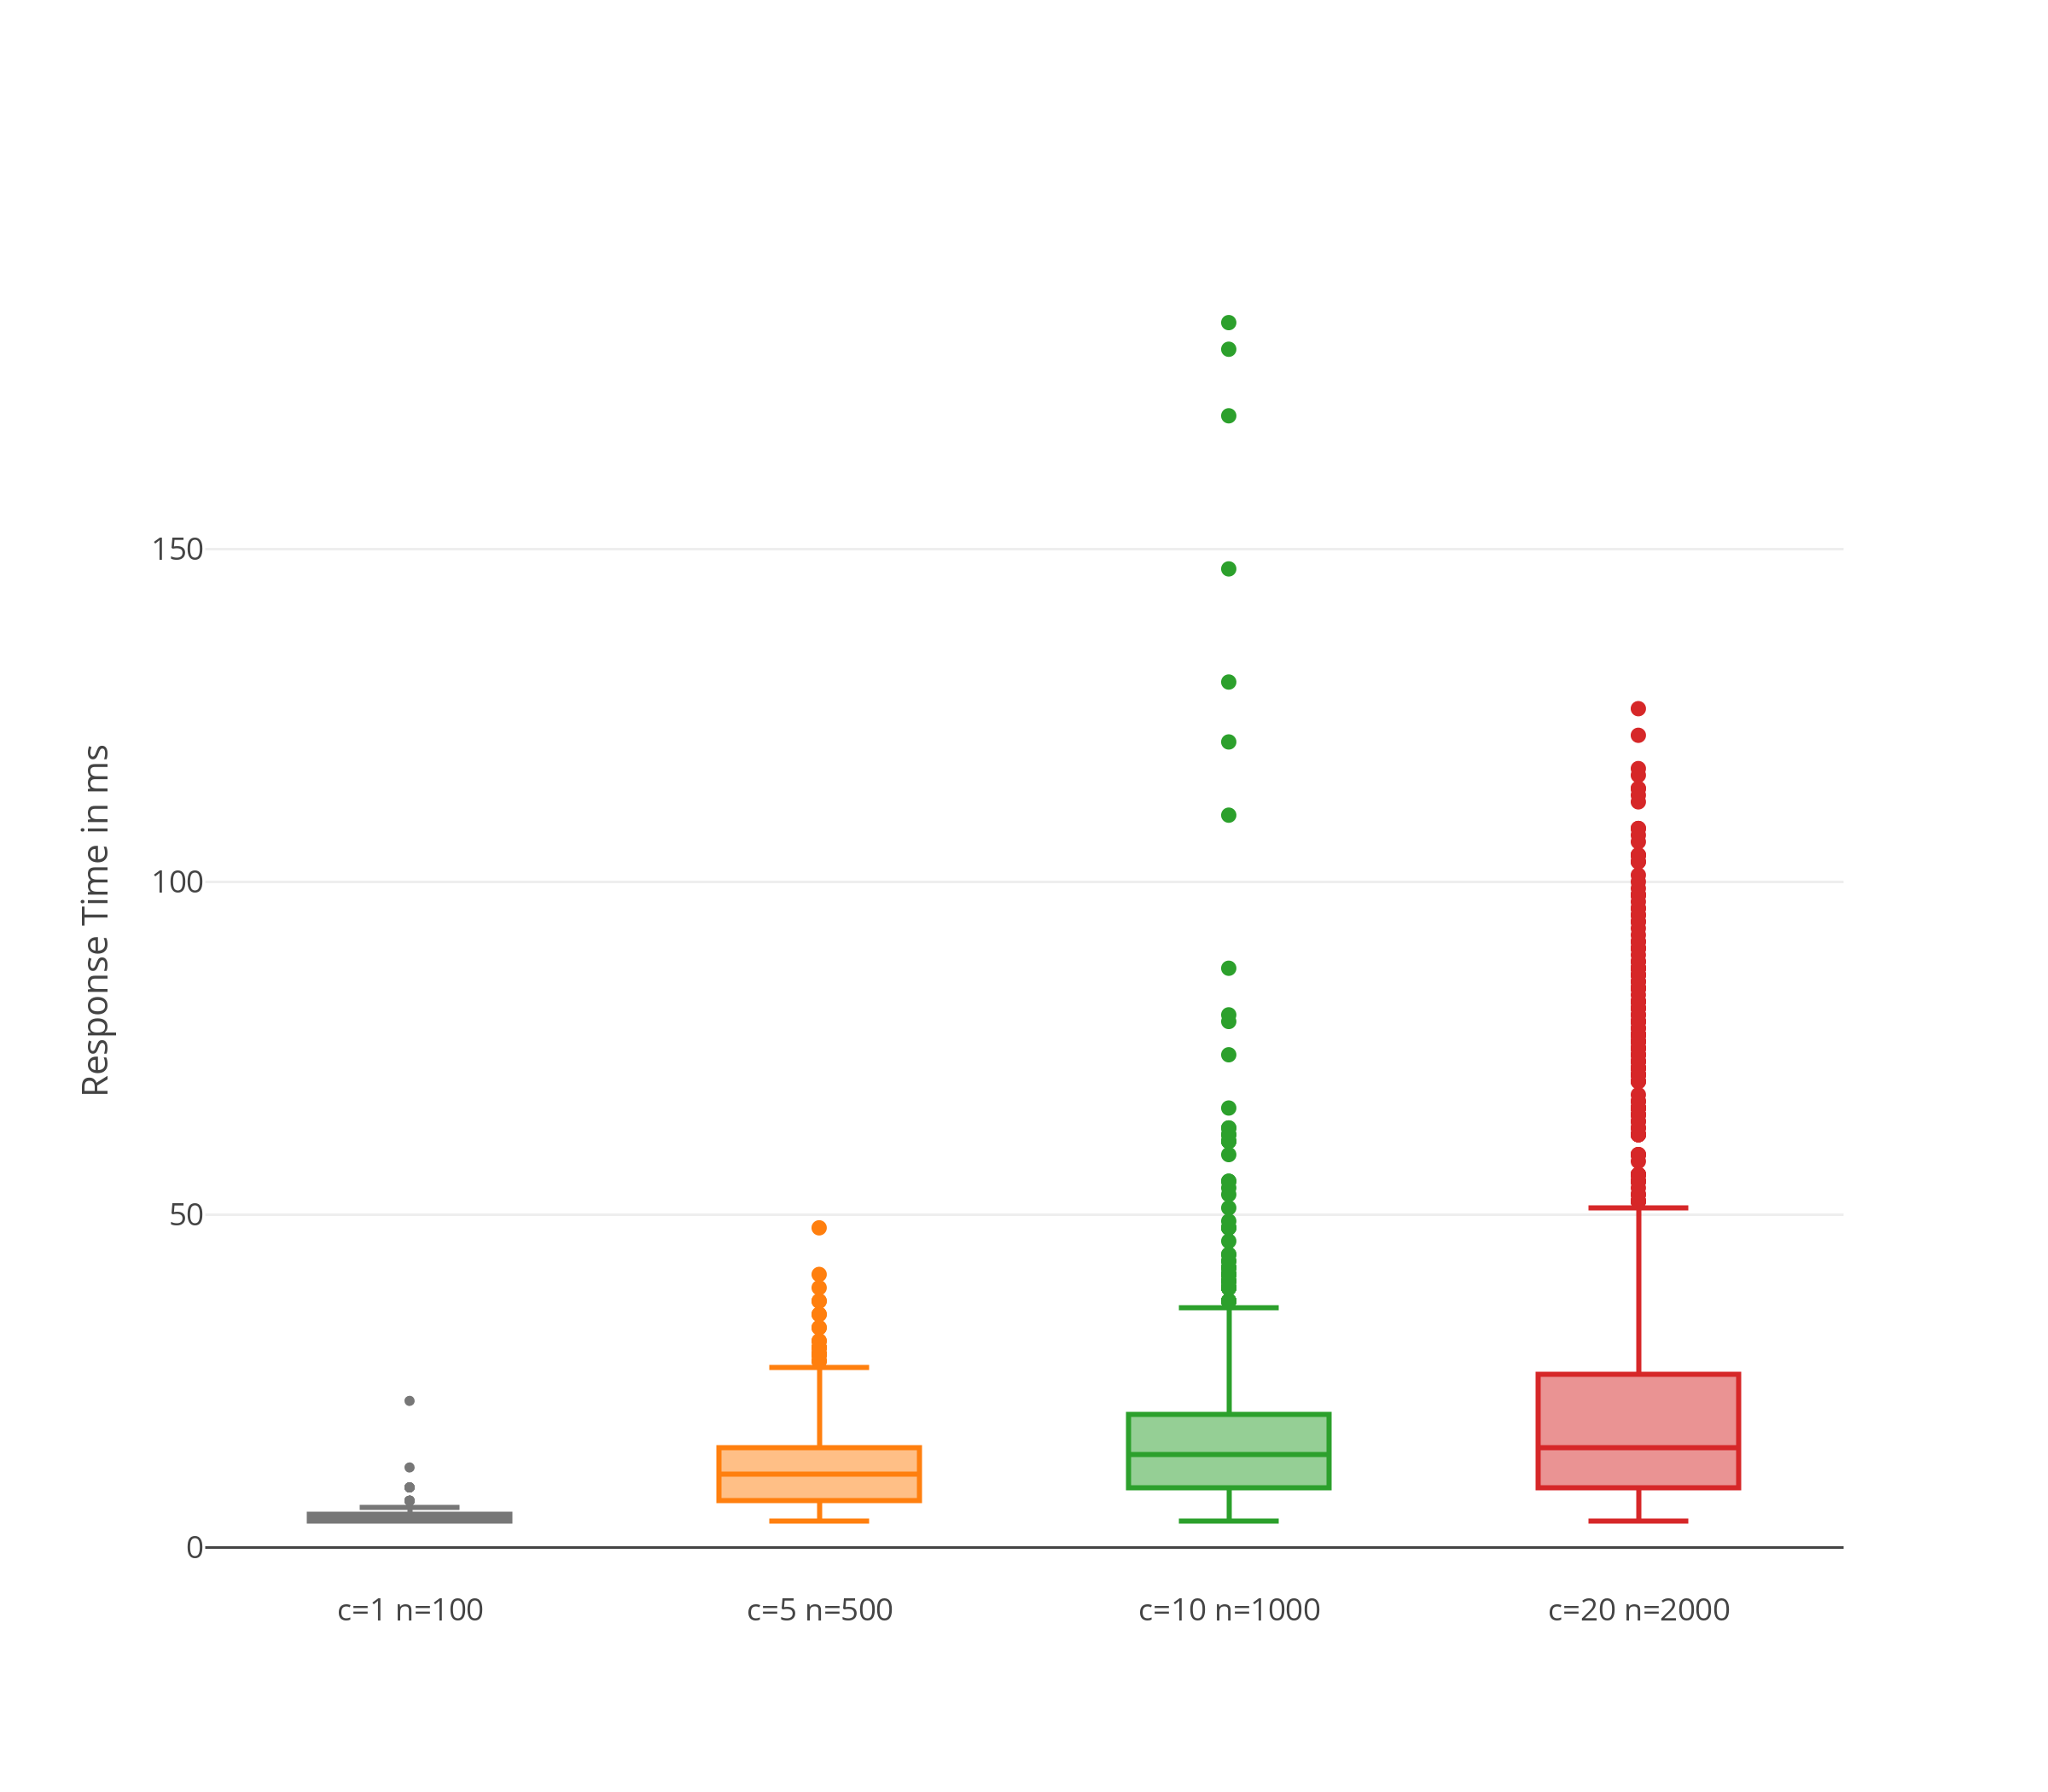
\includegraphics[width=350pt]{Images/ValidateRequestWaitDurationsDiagram.png}
\caption{Graphic representation of the waiting durations until first processing of validation requests in ms.}
\label{fig:ValidateRequestWaitDurationsDiagram}
\end{figure}

\begin{figure}[H]
\centering
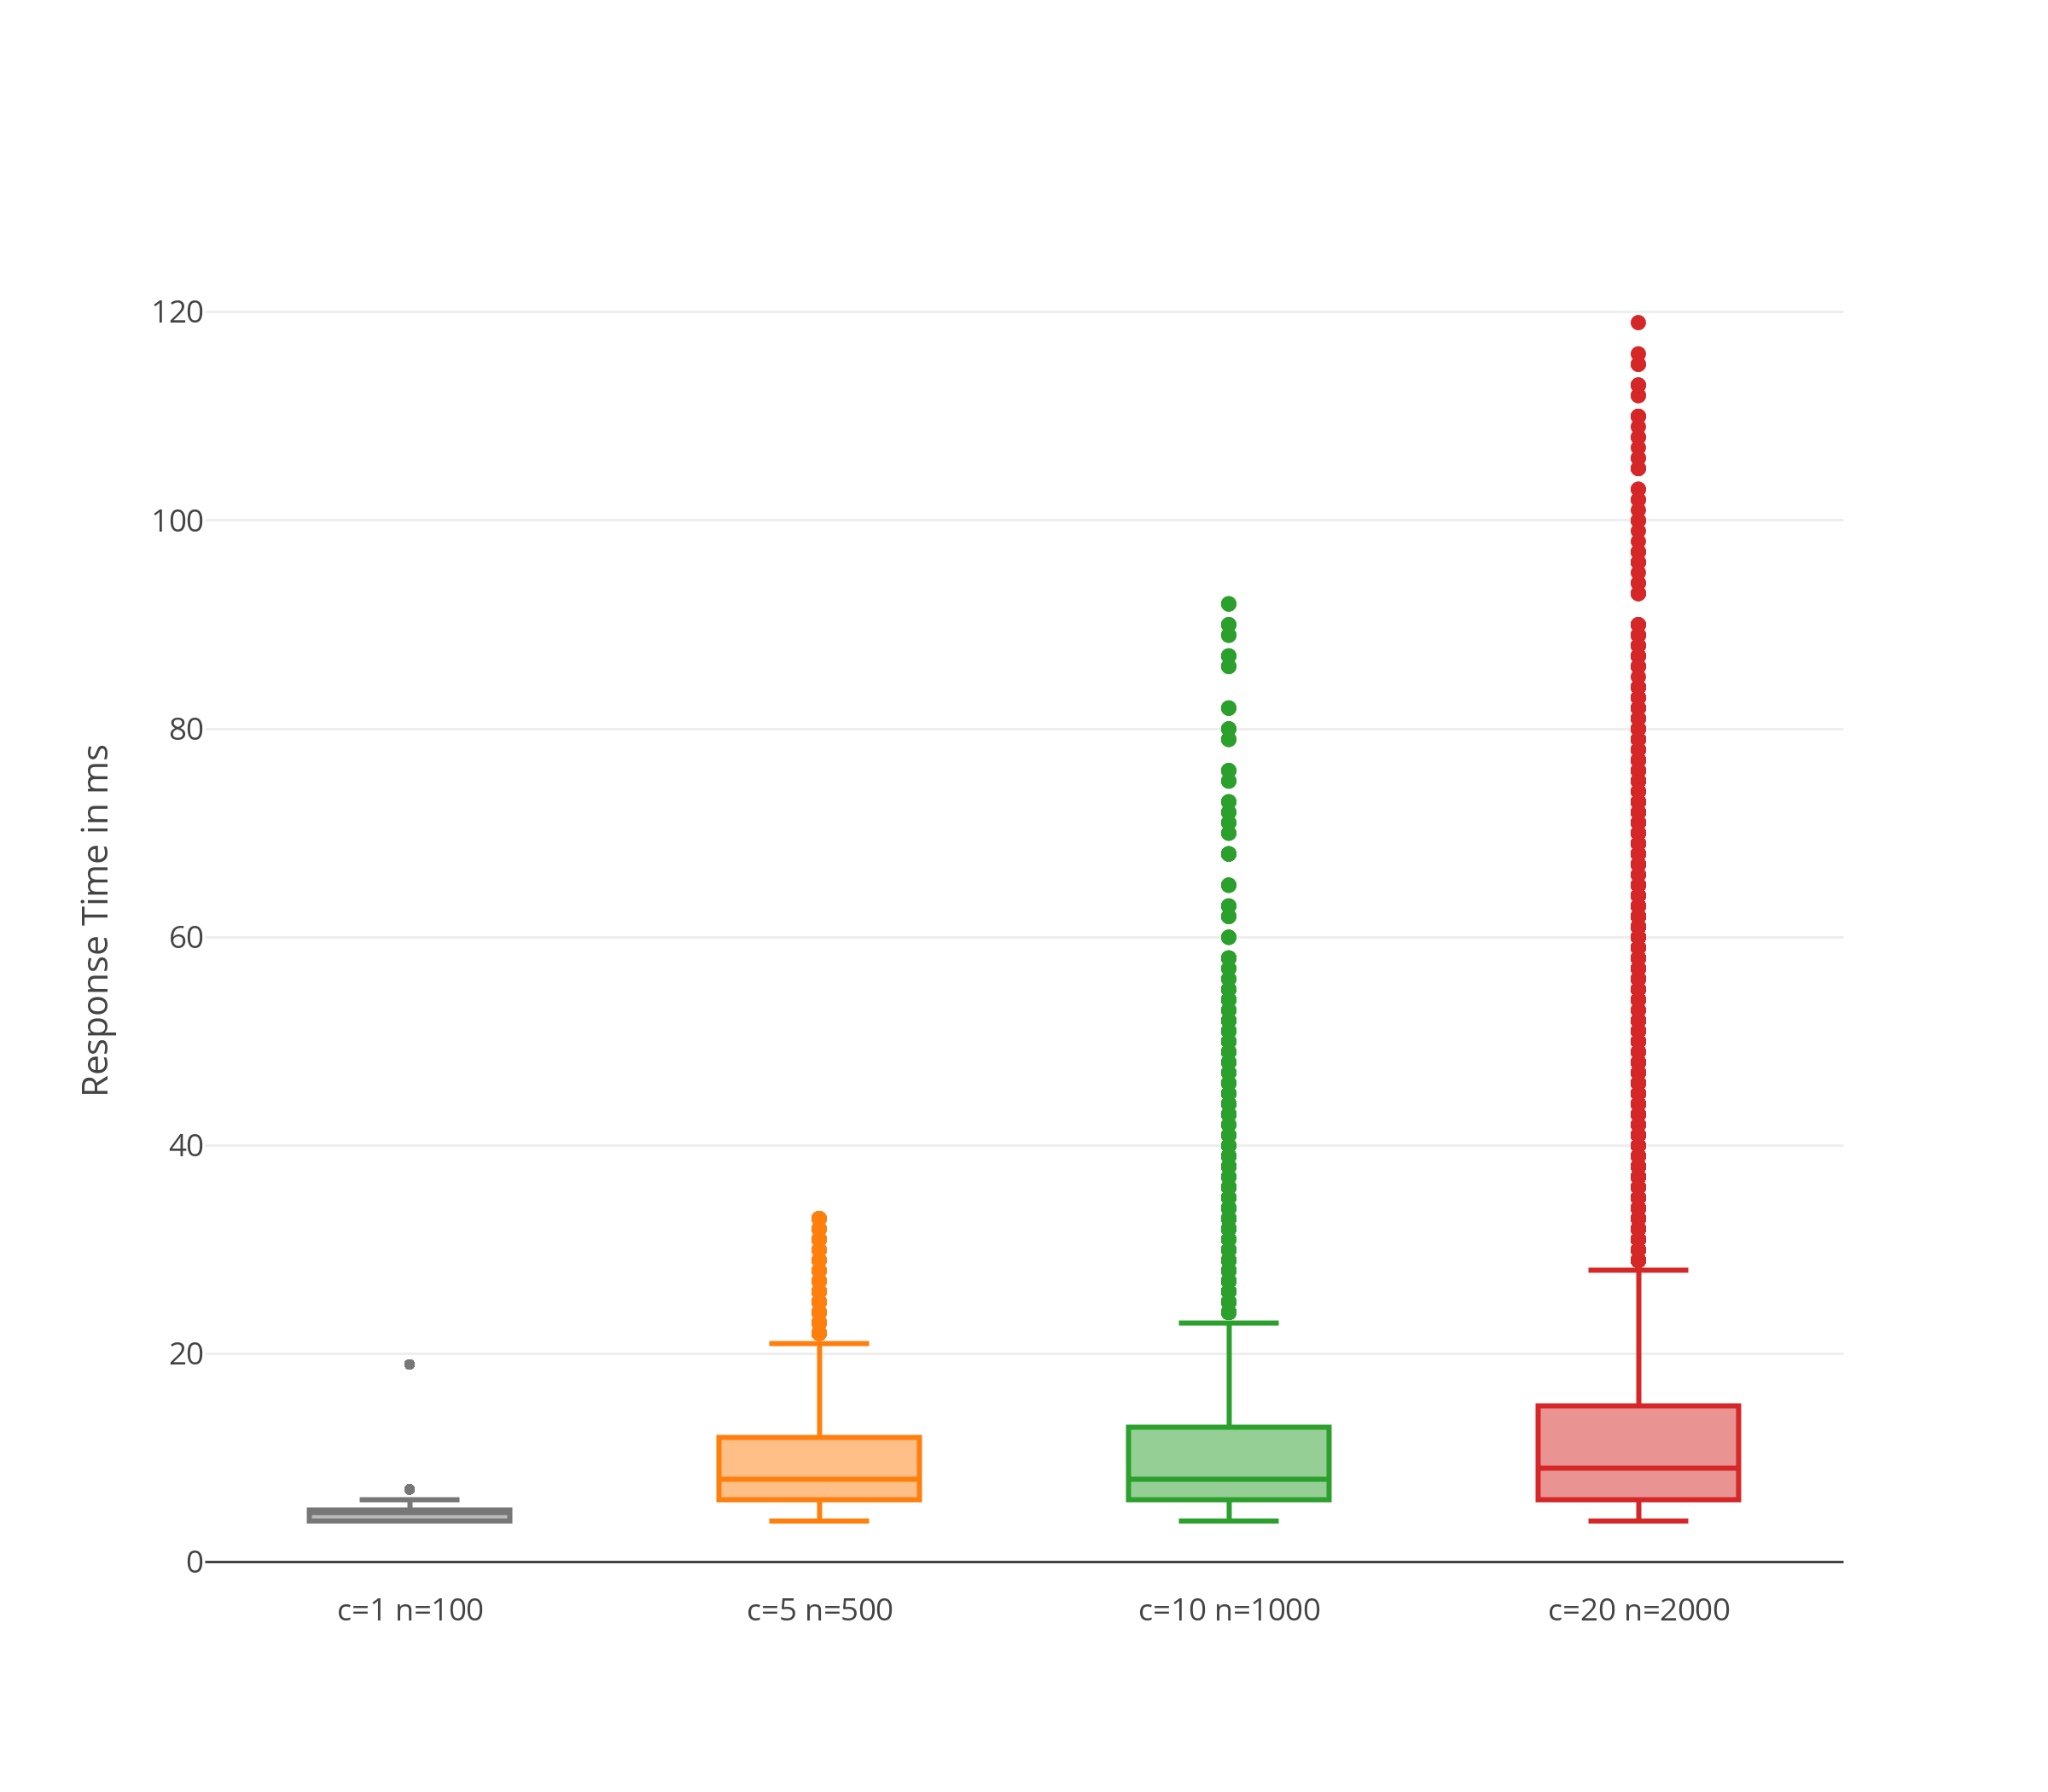
\includegraphics[width=350pt]{Images/CreateSignatureWaitDurationsDiagram.png}
\caption{Graphic representation of the waiting durations until first processing of create-signature requests in ms.}
\label{fig:CreateSignatureWaitDurationsDiagram}
\end{figure}

Since all events for the event loop are recorded in a first-in-first-out (FIFO) queue also all other asynchronous operations are delayed similarly. Assume a simplified case where 20 requests are coming in for verification at once. At first the signature of the first request is checked. Then it needs to check and increase the request counter. This is an asynchronous operation because it involves the Redis database running on a different node. So the server can start processing the signature of the second request in the meantime. Now the result from the Redis is coming back and the task of processing it is added to the end of the event loop queue. This means to continue processing the first request, the node server first needs to verify all other requests signatures because they are in front of it in the queue. This delays the answer of the first request.\\

For the public request to complete four requests to Payment Servers are needed - two for signature creation and two for verification. This means this situation occurs four times per public request and therefore adds up significantly.\\

These effects in combination explain the increased response times when doing a lot of concurrent requests.\\

It is worth noting, that this is not an absolute performance limitation of the system or the blockchain. It is a performance limitation of node.js that can be tackled like any other node.js performance problem. For example, by scaling up the number of instances of the Payment Servers and distributing the load across them. A Payment Server itself is already stateless (it only keeps cached data) and all data that needs to be exchanged can be synchronized via the Redis database.\\
Another solution to the event loop blocking by the cryptographic operations is to perform them in another thread using libraries like Node Webworker Threads \cite{web55}, or even delegating them asynchronously to a dedicated process with an optimized implementation, e.g. written in C.

\newpage
\section{Comparison to Alternative Approaches}

Beside the solution outlined above, other approaches were investigated but not found suitable for the stated requirements. These approaches can be categorized into those involving a blockchain system and those dropping the blockchain approach altogether.

\subsection{Blockchain Based Alternatives}

Achieving the necessary performance of a blockchain based system with other means than state channels seemed not to be feasible.\\

Tuning blockchain parameters like block size and block frequency can improve the performance and throughput for existing blockchain use-cases but cannot achieve latencies in the range of milliseconds.\\

Sidechains and sharding approaches also still rely on consensus mechanisms that are usually too slow for this use-case, although they can significantly increase the transaction volume.\\

Permissioned or private blockchains can achieve higher throughputs and can be more manageable. They can be dedicated to a special purpose, so no other irrelevant transactions need to be processed. If they are of smaller size, other consensus algorithms can be used, too. Byzantine Fault Tolerance algorithms for example can achieve significantly higher throughputs at relatively low latencies \cite{Li2017}.\\
However, this project considered the public use of the payment system as well, so relying solely on improvements through permissioned blockchains did not seem viable. Combining a permissioned blockchain setting with the payment system can, however, improve the latencies for contract deployment, token redemption and payout operations, which enables shorter timeout periods.\\

To solve problems with keeping track of request counters, the Addressable Storage pattern seemed like a possible solution at first. For each request a unique token could be created and stored in an external storage. Once stored, a token cannot be used again. The blockchain would only contain the verification hash and the location of that external storage. However, to check if a token was already used the list of used tokens is needed by the Intermediary smart contract itself and would need to be sent to it every time, which would result in a huge amount of data transfer and computation overhead. Beside this, the verification hash needs to be updated every time a new token is registered as used. This also requires a transaction on the blockchain which incurs transaction fees and latencies.

\subsection{Non Blockchain Based Alternatives}

Moving away from a blockchain solution usually instantly violates the security and trustlessness requirements that were stated earlier. There are for sure use cases that do not demand these challenging requirements, e.g. when all involved parties fully trust each other or the value that shall be protected is insignificant.\\

If the goal would be to only infer dependencies, an approach based on existing tracing systems like Dapper \cite{Sigelman2010} or AWS X-Ray \cite{web41} could be used with smaller performance and complexity impacts.\\
Another traditional approach is the evaluation of logs after the service interactions happened.\\

If a payment processing for requests is the main goal, but the parties trust each other, a system based on a post-processing can yield a significantly higher performance.  This is similar to how cloud computing providers already charge their clients. The client trusts the cloud provider, that he tracks resource usage correctly, and receive an aggregated bill at the end of the payment period. The cloud provider on the other side trusts the client to pay the bill eventually.\\

A compromise solution could be to only partially weaken the requirements. For example, one could try to to not ensure the correct delivery and payment of individual requests, but to guard only larger request batches and tollerate minor counting errors inside a batch. The damage that a malicious actor could do is then limited and the performance impact could be reduced.\\

But neither of these approaches enable a tracing in a fully trustless way, nor do they support a secure pay-per-request model which is key to the proposed system.\\

\newpage
\section{Conclusion and Future Work}

This thesis showed that it is possible to perform high frequency machine-to-machine payments on blockchain systems to model and monitor financial dependencies in microservice architectures. All this without losing essential blockchain properties or tremendous performance issues. Also, stakeholders showed great interest in such a system and were keen on the underlying technologies.\\

However, this prototype is not production and prime-time ready yet. A lot of development effort is needed to mature the system. The stability needs to be improved. Also a solution to scale the number of Payment Servers based on the incoming load must be implemented.\\
Beside this, a major goal must be to make this system easy to use and especially easy to deploy. This was one of the largest concerns of the interviewed stakeholders. They are interested in the data but do not want to invest weeks of integration and setup work. The system must be plug and play. Ideally an automated setup script could be created that takes some input parameters and deploys the required systems for a team to AWS. Technologies like Docker containers and AWS cloud formation templates might be helpful here.\\

One might argue that the current performance overhead is still too large for big enterprise scale microservice architectures. This is a valid concern, however, this is just a prototype and significant improvements can be achieved by speeding up the cryptographic computations. It might even be possible to reduce the overhead to a similar level as encrypting HTTP traffic with TLS \cite{dierks1999rfc}. This should be an acceptable level for many applications, but for sure not for all. In the meantime, this system can also be used to secure only high value services that accept higher latencies and have fewer interactions.\\

The visualizer also needs to evolve into a dashboard, which is able to show graphs and to better visualize the high level flows and interaction patterns, rather than the currently more debugging focused interface. A challenge with this is the performance of the evaluation of the data on the blockchain and might require additional computing and data analytics software.\\

As already mentioned, a lot of future work can be done to mature this system on an operational level. This is not much academic work but well studied software operation and development craftsmanship.\\

In addition to technical investigations, a more business oriented analysis could be performed. It would be interesting to investigate the pricing models and their impacts. Also, how and which market mechanics evolve and what benefits are measurable.\\
A cost breakdown of the system should be performed to evaluate how much cost the payment infrastructure itself creates.\\

Once such a system is in place within a company, external partners of that company could also be billed and tracked through the system. This, of course, might have some legal and taxing issues but it is technically possible. Eventually one could imagine building an open marketplace for services where services pay each other with cryptocurrencies and anyone can offer services, like an AppStore but for web-based backend services.\\
Such a service marketplace is highly related to research and developments in the Software as a Service field and requires further research for legal aspects, service discovery and detailed technical solutions.

\newpage

\bibliography{refs}{}
\bibliographystyle{plain}

\end{document}
